\documentclass[12pt,a4paper,twoside]{book}
% Language setup for Greek and English
\usepackage[english,greek]{babel}
\usepackage[utf8]{inputenc}
\usepackage[T1,LGR]{fontenc}
% Font setup
\usepackage{fontspec}
\setmainfont{Linux Libertine O}[Scale=0.9]
\setsansfont{Linux Biolinum}[Scale=0.9]
\setmonofont{DejaVu Sans Mono}[Scale=0.9]
% Other necessary packages
\usepackage{enumitem}
\usepackage{graphicx}
\usepackage{amsmath}
\usepackage{makeidx}
\usepackage{multicol}
\usepackage{multirow}
\usepackage{adjustbox}
\usepackage{amssymb}
\usepackage{stackengine}
\usepackage{ifthen}
\usepackage{array}
\usepackage{tcolorbox}
\tcbuselibrary{skins,breakable}
\usepackage{minted}
\usepackage{listings}
\usepackage{parskip}
\usepackage{float}
\usepackage{subcaption}
\usepackage{xcolor}
\usepackage{cancel}
\usepackage{pdfpages}
\usepackage{titlesec}
% Bibliography setup
\usepackage[numbers,square,sort\&compress,longnamesfirst]{natbib}

% Define commands for authoryear-style citations
\newcommand{\citeauthyear}[1]{[\citeauthor{#1} \citeyear{#1} \citenum{#1}]}
\newcommand{\Citeauthyear}[1]{\Citeauthor{#1} [\citeyear{#1} \citenum{#1}]}

\makeatletter
\renewenvironment{thebibliography}[1]%
     {\@mkboth{\MakeUppercase\refname}{\MakeUppercase\refname}%
      \list{\@biblabel{\@arabic\c@enumiv}}%
           {\settowidth\labelwidth{\@biblabel{#1}}%
            \leftmargin\labelwidth%
            \advance\leftmargin\labelsep%chktex 41
            \@openbib@code%
            \usecounter{enumiv}%
            \let\p@enumiv\@empty%chktex 21
            \renewcommand\theenumiv{\@arabic\c@enumiv}}%
      \sloppy%
      \clubpenalty4000%
      \@clubpenalty\clubpenalty%
      \widowpenalty4000%
      \sfcode`\.\@m}%chktex 21
     {\def\@noitemerr%chktex 21
        {\@latex@warning{Empty `thebibliography' environment}}%
      \endlist}
\makeatother
% Page & text layout
\usepackage{geometry}
\geometry{
   a4paper,
   top=2.5cm,
   bottom=2.5cm,
   left=2.5cm,
   right=2.5cm
}
% Headers & footers
\usepackage{fancyhdr}
\pagestyle{fancyplain}
\fancyhf{} % Clear all header/footer fields

% Define plain style for chapter pages and TOC
\fancypagestyle{plain}{%
    \fancyhf{} % Clear all header/footer fields
    \renewcommand{\headrulewidth}{0pt} % Remove header rule
    \renewcommand{\footrulewidth}{0pt} % Remove footer rule
}

% Define TOC style with specific headers
\fancypagestyle{tocstyle}{%
    \fancyhf{} % Clear all header/footer fields
    \fancyhead[LE]{\thepage}
    \fancyhead[CE]{\leftmark}
    \fancyhead[CO]{\rightmark}
    \fancyhead[RO]{\thepage}
    \renewcommand{\headrulewidth}{0pt}
}

% Fix marks to prevent premature updates - use extramarks to delay mark updates
\renewcommand{\sectionmark}[1]{\markboth{#1}{}}
\renewcommand{\subsectionmark}[1]{\markright{#1}}

% Redefine \tableofcontents to use tocstyle
\let\oldtableofcontents\tableofcontents
\renewcommand{\tableofcontents}{%
    \clearpage
    % First page of TOC should be empty
    \thispagestyle{empty}
    \pagestyle{tocstyle}
    \oldtableofcontents % chktex 1
    \clearpage
    \pagestyle{fancy}
    % Regular pages header settings
    \fancyhead[LE]{\thepage} % Left header on Even pages: Shows page number
    \fancyhead[CE]{\leftmark} % Center header on Even pages: Shows chapter name (stored in \leftmark)
    \fancyhead[RE]{ΚΕΦ. \thechapter} % Right header on Even pages: Shows "ΚΕΦ." followed by chapter number % chktex 12

    \fancyhead[LO]{\thesection} % Left header on Odd pages: Shows current section number
    \fancyhead[CO]{\rightmark} % Center header on Odd pages: Shows section name (stored in \rightmark)
    \fancyhead[RO]{\thepage} % Right header on Odd pages: Shows page number

    \renewcommand{\headrulewidth}{0.4pt} % Sets thickness of the horizontal line below the header

    % Redefine chapter mark to remove "Chapter" prefix
    \renewcommand{\chaptermark}[1]{\markboth{##1}{}}
    % Redefine section mark to delay updates until after page break
    % This prevents showing the next section number when current section ends at page bottom
    \renewcommand{\sectionmark}[1]{%
        \markright{##1}%
    }
    \renewcommand{\subsectionmark}[1]{}
}

% Additional fix: Make section marks update at first mark instead of both marks
\makeatletter
\renewcommand\sectionmark[1]{%
  \markright{%
    \ifnum \c@secnumdepth >\z@
      \thesection\quad
    \fi
    #1}}
\makeatother

% Make table of contents use plain style
\addtocontents{toc}{\protect\thispagestyle{plain}}

% Hyperlinks
\usepackage{hyperref}
\usepackage{bookmark}                                       % Add this line to fix the hyperref warnings
\hypersetup{
    colorlinks=true,
    linkcolor=blue,
    citecolor=blue,
    filecolor=blue,
    urlcolor=customCodeBlue,
    unicode,
    pdftitle={Ταξινόμηση Ανεπιθύμητων Email}, % chktex 19
    pdfsubject={Αναφορά Εργασίας},
    pdfborderstyle={/S/U/W 1},                              % Underline links
}
\usepackage{tikz}
\usetikzlibrary{positioning, shapes.geometric, arrows.meta}
\usepackage{pgfplots}
\pgfplotsset{compat=1.18}
\usetikzlibrary{calc,arrows.meta,positioning}

\definecolor{customRed}{HTML}{FF5F5A}                       % using hexadecimal
\definecolor{customYellow}{HTML}{FFBE2E}                    % using hexadecimal
\definecolor{customGreen}{HTML}{2ACA44}                     % using hexadecimal
\definecolor{customPurple}{HTML}{C477DB}                    % using hexadecimal
\definecolor{customBlue}{HTML}{052538}                      % using hexadecimal
\definecolor{customLightBlue}{HTML}{60ADEC}                 % using hexadecimal
\definecolor{customGray}{HTML}{A0A0A0}                      % using hexadecimal
\definecolor{customBlack}{HTML}{000000}                     % using hexadecimal

% Define a lighter gray for background and darker colors for text
\definecolor{customBgGray}{HTML}{E0E0E0}         % Light gray background
\definecolor{customCodeRed}{HTML}{C92A2A}        % Darker red
\definecolor{customCodeYellow}{HTML}{E67700}     % Darker yellow/orange
\definecolor{customCodeGreen}{HTML}{087F23}      % Darker green
\definecolor{customCodePurple}{HTML}{7B1FA2}     % Darker purple
\definecolor{customCodeBlue}{HTML}{1976D2}       % Darker blue
\definecolor{customCodeBlack}{HTML}{1A1A1A}      % Lighter black

\lstdefinestyle{myPythonStyle}{
    language=Python,                                            % Set the language to Python
    backgroundcolor=\color{customBgGray},                       % Background color
    basicstyle=\color{customCodeBlack}\ttfamily\footnotesize,   % Basic font style, size, and color
    keywordstyle=\color{customCodePurple}\bfseries,             % Style for general keywords
    keywordstyle=[2]\color{customCodeYellow}\bfseries,          % Style for specific keywords
    commentstyle=\color{customCodeGreen}\itshape,               % Style for comments
    stringstyle=\color{customCodeGreen},                        % Style for strings
    identifierstyle=\color{customCodeBlue},                     % Style for identifiers
    morekeywords={self, None, True, False, format, abs,
                as, pass, return, if, elif, else, for,
                range, while, try, except, with, lambda,
                yield, global, nonlocal, assert, del,
                raise, in, is, and, or, not},                   % Additional keywords
    morekeywords=[2]{os, graphviz, Digraph, collections,
                    deque, math, tabulate, join, sub, lower, split, MULTILINE, CountVectorizer, fit_transform, transform,encode, SentenceTransformer},                     % Define 'import' and 'from' as additional keywords
    % procnamekeys={def,class},                                 % Highlight function and class names
    showstringspaces=false,                                     % Don't show spaces in strings
%
    breaklines=true,                                            % Automatically break long lines
    breakatwhitespace=false,                                    % Break lines at any character
    % prebreak=\textbackslash,                                  % Character for breaking lines
    postbreak={\space},                                         % Character for breaking lines
    breakautoindent=false,                                      % Indentation after line break
    breakindent=0pt,                                            % Indentation before line break
    resetmargins=true,                                          % Reset margins after line break
    keepspaces=true,                                            % Keep spaces in the code
    showspaces=false,                                           % Don't show spaces
    columns=flexible,                                           % Column format
%
    numbers=left,                                               % Line numbers on the left
    numberstyle=\small\color{customBgGray},                     % Style for line numbers
    % numwidth=4em,                                             % Width allocated for line numbers
    stepnumber=1,                                               % Step between line numbers
    numbersep=8pt,                                              % Distance of line numbers from code
    xleftmargin=1.5em,                                          % Match the numwidth
    tabsize=4,                                                  % Size of a tab
    captionpos=t,                                               % Position of the caption (t for top)
    firstnumber=auto,                                           % Continue line numbering from previous listing
    aboveskip=0em,                                              % Remove external spacing
    belowskip=0em,                                              % Remove external spacing
    frame=none,                                                 % Add top and bottom rules only
    framerule=0pt,                                              % Make the rules invisible
    rulecolor=\color{customBgGray},                             % Color of the frame (if enabled)
    framesep=2pt,                                               % Add internal padding
    % framexleftmargin=1em,                                     % Add internal left margin
    % framexrightmargin=1em,                                    % Add internal right margin
    escapeinside={\(*@}{@*\)},                                  % For escaping characters
    morecomment=[l]{\#},                                        % Define comment style
    morestring=[b]',                                            % Define string style with single quotes
    morestring=[b]",                                            % Define string style with double quotes % chktex 18
    literate={
        {``}{{\textquotedbleft}}2
        {''}{{\textquotedbright}}2
        {`}{{\textquoteleft}}1
        {'}{{\textquoteright}}1
        {_}{{\_}}1
    },
}

\lstdefinestyle{myCStyle}{
    language=C,
    backgroundcolor=\color{customBgGray},                       % Background color
    basicstyle=\color{customCodeBlack}\ttfamily\footnotesize,   % Basic font style
    keywordstyle=\color{customCodePurple}\bfseries,            % Style for keywords
    keywordstyle=[2]\color{customCodeYellow}\bfseries,         % Style for additional keywords
    commentstyle=\color{customCodeGreen}\itshape,              % Style for comments
    stringstyle=\color{customCodeGreen},                       % Style for strings
    identifierstyle=\color{customCodeBlue},                    % Style for identifiers
    morekeywords={void, int, char, float, double, long, short, signed, unsigned,
                  const, static, extern, volatile, register, auto, struct, union,
                  typedef, enum, sizeof, break, continue, goto, return, if, else,
                  switch, case, default, for, while, do, pid_t, sem_t},
    morekeywords=[2]{stdio.h, stdlib.h, string.h, math.h, time.h, ctype.h,
                     unistd.h, semaphore.h, sys/mman.h, sys/wait.h, fcntl.h,
                     printf, fprintf, perror, exit, malloc, free, fork, waitpid,
                     mmap, munmap, sem_init, sem_wait, sem_post, sem_destroy,
                     sleep, rand, srand, atoi, time, MAP_SHARED, MAP_ANONYMOUS,
                     PROT_READ, PROT_WRITE, MAP_FAILED, EXIT_SUCCESS, EXIT_FAILURE},
    showstringspaces=false,
    frame=none,
    rulecolor=\color{customBgGray},
    breaklines=true,                % Break long lines
    breakatwhitespace=false,        % Break at any character
    postbreak={\space},             % Character after break
    breakautoindent=false,          % No indentation after break
    breakindent=0pt,                % No indent before break
    resetmargins=true,              % Reset margins after break
    keepspaces=true,                % Preserve spaces
    showspaces=false,               % Don't show spaces
    columns=flexible,               % Column format
    numbers=left,
    numberstyle=\small\color{customBgGray},
    stepnumber=1,
    numbersep=8pt,
    xleftmargin=1.5em,
    tabsize=4,
    captionpos=t,
    firstnumber=auto,
    aboveskip=0em,
    belowskip=0em,
    framesep=2pt,
    escapeinside={\(*@}{@*\)},
    morecomment=[l]{//},
    morecomment=[s]{/*}{*/},
    morestring=[b]", % chktex 18
    morestring=[b]',
    literate={
        {``}{{\textquotedbleft}}2
        {''}{{\textquotedbright}}2
        {`}{{\textquoteleft}}1
        {'}{{\textquoteright}}1
        {_}{{\_}}1
    },
}

\lstdefinestyle{myBashStyle}{
    language=bash,
    backgroundcolor=\color{customBgGray},                       % Background color
    basicstyle=\color{customCodeBlack}\ttfamily\footnotesize,   % Basic font style
    keywordstyle=\color{customCodePurple}\bfseries,            % Style for keywords
    keywordstyle=[2]\color{customCodeYellow}\bfseries,         % Style for additional keywords
    commentstyle=\color{customCodeGreen}\itshape,              % Style for comments
    stringstyle=\color{customCodeGreen},                       % Style for strings
    identifierstyle=\color{customCodeBlue},                    % Style for identifiers
    alsoletter={0123456789}                                    % Define numbers as letters
    morekeywords={if, then, else, elif, fi, for, while, do, done, in, case, esac, 
                  function, select, until, break, continue, return, exit, shift,
                  declare, local, readonly, export, set, unset},
    morekeywords=[2]{echo, read, cat, awk, grep, sed, cut, tr, sort, uniq, wc,
                     mkdir, rm, cp, mv, ls, cd, pwd, touch, chmod, chown, find,
                     test, source, alias, eval, exec, getopts, printf, wait,
                     STDIN, STDOUT, STDERR, IFS, PATH, BEGIN, END, NR, NF, 
                     tolower, concat, print},
    showstringspaces=false,
    frame=none,
    rulecolor=\color{customBgGray},
    breaklines=true,                % Break long lines
    breakatwhitespace=false,        % Break at any character
    postbreak={\space},             % Character after break
    breakautoindent=false,          % No indentation after break
    breakindent=0pt,                % No indent before break
    resetmargins=true,              % Reset margins after break
    keepspaces=true,                % Preserve spaces
    showspaces=false,               % Don't show spaces
    columns=flexible,               % Column format
    numbers=left,
    numberstyle=\small\color{customBgGray},
    stepnumber=1,
    numbersep=8pt,
    xleftmargin=1.5em,
    tabsize=4,
    captionpos=t,
    firstnumber=auto,
    aboveskip=0em,
    belowskip=0em,
    framesep=2pt,
    escapeinside={\(*@}{@*\)},
    morecomment=[l]{\#},
    morestring=[b]", % chktex 18
    morestring=[b]',
    literate={
        {``}{{\textquotedbleft}}2
        {''}{{\textquotedbright}}2
        {`}{{\textquoteleft}}1
        {'}{{\textquoteright}}1
        {_}{{\_}}1
    },
}

\tcbset{
    myCustomStyle/.style={
        enhanced,                       % Enable enhanced features
        breakable,                      % Allow the box to break across pages
        colback=customBlue,             % Background color
        colframe=customBgGray,              % Frame color
        listing only,                   % Use listings
%
        fonttitle=\bfseries,            % Title font style
        % frame=single,                 % Frame type
        % interior titled,              % Use regular titled interior
        interior style={
            top color=black!75,         % Title area background
            bottom color=black!75,      % Title area background
        },
        colbacktitle=black!75,          % Title background color
        coltitle=white,                 % Title color
        rounded corners,                % Rounded corners
        boxrule=1mm,                    % Frame thickness
        drop shadow southeast,          % Shadow effect
        lefttitle=0pt,                  % Remove left margin of title
        % left=1em,                     % Increase left margin for line numbers
        title={\hspace*{-1em}\textcolor{customRed}{● }\textcolor{customYellow}{● }\textcolor{customGreen}{●}\quad#1}, % Circles + Title
        attach title to upper={\vspace{2.3mm}}, % Adjust vertical spacing
%
        beforeafter skip=8pt,           % Space before and after the box
        breaklines=true,                % Allow the box to break across pages
        breakatwhitespace=false,        % Break lines at any character if necessary
        % sharp corners                 % Sharp corners for the title area
    }
}

% Custom commands for language switching
\newcommand{\en}[1]{\foreignlanguage{english}{#1}}
\newcommand{\gr}[1]{\foreignlanguage{greek}{#1}}
% Custom command for coloring
\newcommand{\blue}[1]{\textcolor{blue}{#1}}
% Index
\makeindex
% Set headheight to avoid fancyhdr warnings
\setlength{\headheight}{14.5pt}

% Adjust chapter spacing
\titleformat{\chapter}[display]
{\normalfont\huge\bfseries}{\chaptertitlename\ \thechapter}{15pt}{\Huge}
\titlespacing*{\chapter}{0pt}{-10pt}{20pt}

% Adjust section spacing
\titlespacing*{\section}{0pt}{10pt}{10pt}

% Adjust vertical space between paragraphs
\setlength{\parskip}{0.5em}

% Make figure placement less strict
\setcounter{topnumber}{2}
\setcounter{bottomnumber}{2}
\setcounter{totalnumber}{4}
\renewcommand{\topfraction}{0.85}
\renewcommand{\bottomfraction}{0.85}
\renewcommand{\textfraction}{0.15}
\renewcommand{\floatpagefraction}{0.7}

\begin{document}
% Start Arabic numbering from the beginning but hide numbers
\pagenumbering{arabic}
% Add this command to prevent blank pages
\let\cleardoublepage\clearpage

% Set main language to Greek
\selectlanguage{greek}

% Document information
\title{Ταξινόμηση Ανεπιθύμητων Email (Spam Classification)}
\author{Μπίτζας Βασίλειος}
\date{\today}

% Title page with hidden number
\begin{titlepage}
    \vspace*{5cm}
    \begin{center}
        
\includegraphics[width=0.3\textwidth]{media/logo.png}\\
        \vspace*{1cm}
        {\LARGE \textbf{\textit{Ταξινόμηση Ανεπιθύμητων Email}}}\\ % chktex 8
        \vspace*{0.5cm}
        {\large Στατιστικές Μέθοδοι Μηχανικής Μάθησης} % chktex 19
        \vspace*{5cm}
        \\
        \vspace*{1cm}
        \begin{tabular}{l l l}
            \large Βασίλειος Μπίτζας & \large 1083796 & \large up1083796@ac.upatras.gr
        \end{tabular}

        \vspace*{1cm}

        {\normalsize Τμήμα Μηχανικών Ηλεκτρονικών Υπολογιστών \& Πληροφορικής}
        \\
        {\normalsize Πανεπιστήμιο Πατρών}
        \\
    \end{center}
    \thispagestyle{empty} % Suppress page number on the title page
\end{titlepage}

% % Add this command to prevent blank pages
% \let\cleardoublepage\clearpage
% \frontmatter
\tableofcontents
\listoffigures
\listoftables
% \mainmatter % chktex 1

%=============================================================================
% ΚΕΦΑΛΑΙΟ 1: ΕΙΣΑΓΩΓΗ
%=============================================================================
\chapter{Εισαγωγή}

\section{Εισαγωγή}

Το ηλεκτρονικό ταχυδρομείο (email) αποτελεί έναν από τους πιο διαδεδομένους τρόπους επικοινωνίας στον ψηφιακό κόσμο, με περισσότερα από 4 δισεκατομμύρια χρήστες παγκοσμίως. Ωστόσο, η ευρεία χρήση του email έχει οδηγήσει σε ένα σοβαρό πρόβλημα: το \textbf{spam} (ανεπιθύμητα μηνύματα). Σύμφωνα με στατιστικά στοιχεία, περίπου το 45\% έως 50\% όλων των email είναι spam, προκαλώντας σημαντικά προβλήματα στους χρήστες και τις επιχειρήσεις.

Το spam δεν είναι απλώς μια ενόχληση. Περιλαμβάνει διαφημιστικά μηνύματα, απόπειρες ηλεκτρονικού ψαρέματος (phishing), κακόβουλο λογισμικό (malware), και άλλες απειλές που μπορούν να θέσουν σε κίνδυνο την ασφάλεια και την ιδιωτικότητα των χρηστών. Επιπλέον, το spam καταναλώνει σημαντικούς πόρους δικτύου και αποθηκευτικού χώρου, ενώ μειώνει την παραγωγικότητα των χρηστών που αναγκάζονται να ξοδεύουν χρόνο φιλτράροντας ανεπιθύμητα μηνύματα.

Η \textbf{αυτόματη ανίχνευση spam} (spam detection) έχει γίνει κρίσιμη ανάγκη. Οι παραδοσιακές μέθοδοι βασισμένες σε κανόνες (rule-based systems) δεν μπορούν να ανταπεξέλθουν στην εξέλιξη των τεχνικών spam, καθώς οι αποστολείς spam προσαρμόζονται συνεχώς για να παρακάμψουν τα φίλτρα. Αντίθετα, οι \textbf{τεχνικές μηχανικής μάθησης} (machine learning) προσφέρουν μια πιο ευέλικτη και προσαρμοστική προσέγγιση, μαθαίνοντας αυτόματα από παραδείγματα και βελτιώνοντας συνεχώς την απόδοσή τους.

Η παρούσα εργασία επικεντρώνεται στην \textbf{ταξινόμηση email} ως spam ή ham (legitimate email) χρησιμοποιώντας σύγχρονες τεχνικές μηχανικής μάθησης και επεξεργασίας φυσικής γλώσσας (Natural Language Processing - NLP). Συγκεκριμένα, εξετάζουμε διαφορετικές μεθόδους αναπαράστασης κειμένου (Bag-of-Words και Sentence Embeddings) και εφαρμόζουμε διάφορους αλγορίθμους ταξινόμησης (Naive Bayes, k-Nearest Neighbors, Support Vector Machines, Logistic Regression) για να αξιολογήσουμε την αποτελεσματικότητά τους.

\section{Στόχοι Εργασίας}

Η παρούσα εργασία έχει τους ακόλουθους βασικούς στόχους:

\begin{enumerate}
    \item \textbf{Υλοποίηση Pipeline Προεπεξεργασίας Κειμένου}
          \begin{itemize}
              \item Καθαρισμός κειμένου (αφαίρεση URLs, ειδικών χαρακτήρων)
              \item Κανονικοποίηση (μετατροπή σε πεζά, κανονικοποίηση κενών)
              \item Αφαίρεση stopwords από το κείμενο των email
              \item Αξιολόγηση της επίδρασης της προεπεξεργασίας στην απόδοση
          \end{itemize}

    \item \textbf{Σύγκριση Μεθόδων Αναπαράστασης Κειμένου}
          \begin{itemize}
              \item \textbf{Bag-of-Words (BoW)}: Παραδοσιακή προσέγγιση βασισμένη σε συχνότητες λέξεων
              \item \textbf{Sentence Embeddings}: Σύγχρονη προσέγγιση χρησιμοποιώντας pre-trained transformers (all-MiniLM-L6-v2)
              \item Αξιολόγηση της σχέσης απόδοσης/πολυπλοκότητας για κάθε μέθοδο
          \end{itemize}

    \item \textbf{Εφαρμογή και Σύγκριση Αλγορίθμων Ταξινόμησης}
          \begin{itemize}
              \item \textbf{Naive Bayes}: Πιθανοτικός ταξινομητής για baseline comparison
              \item \textbf{k-Nearest Neighbors (k-NN)}: Instance-based learning
              \item \textbf{Support Vector Machines (SVM)}: Με linear και RBF kernels
              \item \textbf{Logistic Regression}: Γραμμικό μοντέλο με L2 regularization
              \item Αξιολόγηση με πολλαπλές μετρικές (Precision, Recall, F1-Score, ROC-AUC)
          \end{itemize}

    \item \textbf{Μελέτη Επίδρασης Μείωσης Διαστάσεων}
          \begin{itemize}
              \item Εφαρμογή Principal Component Analysis (PCA) στα sentence embeddings
              \item Δοκιμή διαφορετικών variance ratios (90\%, 95\%, 99\%) και σταθερών components (10)
              \item Ανάλυση του trade-off μεταξύ μείωσης διαστάσεων και απώλειας απόδοσης
          \end{itemize}

    \item \textbf{Αξιολόγηση και Σύγκριση Μοντέλων}
          \begin{itemize}
              \item Συγκριτική ανάλυση όλων των συνδυασμών (αναπαραστάσεις × αλγόριθμοι × PCA)
              \item Ανάλυση σφαλμάτων (confusion matrices, ROC curves)
              \item Προσδιορισμός του βέλτιστου μοντέλου για διαφορετικά use cases
          \end{itemize}

    \item \textbf{Πρακτικές Συστάσεις}
          \begin{itemize}
              \item Προτάσεις για deployment σε production περιβάλλον
              \item Ανάλυση υπολογιστικής πολυπλοκότητας και scalability
              \item Προτάσεις για μελλοντικές βελτιώσεις
          \end{itemize}
\end{enumerate}

Η εργασία στοχεύει στην παροχή μιας ολοκληρωμένης ανάλυσης των σύγχρονων τεχνικών για την ανίχνευση spam, παρέχοντας τόσο θεωρητική κατανόηση όσο και πρακτική εφαρμογή.

\section{Περιγραφή Δεδομένων}

\subsection{Dataset: emails.csv}

Για την υλοποίηση της εργασίας χρησιμοποιείται το dataset \textit{emails.csv}, το οποίο περιέχει συλλογή email με τα ακόλουθα χαρακτηριστικά:

\begin{itemize}
    \item \textbf{Μέγεθος Dataset}: Σύνολο 5,728 emails
    \item \textbf{Στήλες}:
          \begin{itemize}
              \item \textit{text}: Το περιεχόμενο του email (string)
              \item \textit{spam}: Η ετικέτα κλάσης (binary: 0 = ham, 1 = spam)
          \end{itemize}
    \item \textbf{Κατανομή Κλάσεων}:
          \begin{itemize}
              \item Ham (legitimate emails): 4,360 δείγματα (76.1\%)
              \item Spam (unwanted emails): 1,368 δείγματα (23.9\%)
          \end{itemize}
    \item \textbf{Ποικιλία Περιεχομένου}: Τα email περιλαμβάνουν διάφορους τύπους spam:
          \begin{itemize}
              \item Διαφημιστικά μηνύματα (product promotions)
              \item Οικονομικές απάτες (financial scams)
              \item Προσφορές φαρμάκων (pharmaceutical spam)
              \item Phishing attempts
          \end{itemize}
    \item \textbf{Πραγματικά Δεδομένα}: Το dataset προέρχεται από πραγματικά email, διατηρώντας τη φυσική ποικιλομορφία και πολυπλοκότητα της γλώσσας.
\end{itemize}

\subsection{Διαχωρισμός Dataset}

Το dataset χωρίζεται σε τρία υποσύνολα για την εκπαίδευση και αξιολόγηση των μοντέλων:

\begin{itemize}
    \item \textbf{Training Set}: 4,582 emails (80\% του συνόλου)
          \begin{itemize}
              \item Χρησιμοποιείται για την εκπαίδευση των μοντέλων
              \item Ham: 3,468 emails (75.69\%)
              \item Spam: 1,114 emails (24.31\%)
          \end{itemize}

    \item \textbf{Validation Set}: 572 emails (10\% του συνόλου)
          \begin{itemize}
              \item Χρησιμοποιείται για την επιλογή hyperparameters
              \item Ham: 446 emails (77.97\%)
              \item Spam: 126 emails (22.03\%)
          \end{itemize}

    \item \textbf{Test Set}: 574 emails (10\% του συνόλου)
          \begin{itemize}
              \item Χρησιμοποιείται για την τελική αξιολόγηση
              \item Ham: 446 emails (77.70\%)
              \item Spam: 128 emails (22.30\%)
          \end{itemize}
\end{itemize}

\textbf{Σημείωση}: Πριν τον διαχωρισμό, το dataset ανακατεύεται τυχαία (shuffle) με \textit{random\_state=42} για αναπαραγωγιμότητα των αποτελεσμάτων και για να διασφαλιστεί ότι κάθε υποσύνολο περιέχει αντιπροσωπευτική κατανομή των κλάσεων.

\subsection{Παράδειγμα Δεδομένων}

Τα email στο dataset περιέχουν το θέμα (subject) και το σώμα του μηνύματος. Παράδειγμα spam email:

\begin{tcolorbox}[colback=customBgGray!30, colframe=customCodeRed, title=Παράδειγμα Spam Email]
    \small
    \textit{Subject: vaal medz how t pestilent o save on your medlcations over 70\% . phar anthropoid mshop - suc mucilage cessfull and proven way to save your mo impendence ney . gauleiter v a jauntily g flection al l woodbind u natural l metcast rac selachian l i...}
\end{tcolorbox}

Παράδειγμα ham (legitimate) email:

\begin{tcolorbox}[colback=customBgGray!30, colframe=customCodeGreen, title=Παράδειγμα Ham Email]
    \small
    \textit{Subject: re : hello vince thank you for the update . i will be back in the office january 8 . have a great new year gerry - - - - - original message - - - - - from : vince . j . kaminski @ enron . com [ mailto : vince . j . kaminski @ enron . com ] sent : thursday , december 21 , 2000 5 : 35 pm to : gsheble @ iastate . edu cc : vince...}
\end{tcolorbox}

\section{Διάρθωση Αναφοράς}

Η αναφορά οργανώνεται ως εξής:

\begin{itemize}
    \item \textbf{Κεφάλαιο 2}: Παρουσιάζεται το θεωρητικό υπόβαθρο των αλγορίθμων μηχανικής μάθησης που χρησιμοποιούνται.
    \item \textbf{Κεφάλαιο 3}: Περιγράφεται η μεθοδολογία που ακολουθήθηκε για την επεξεργασία δεδομένων και την εκπαίδευση μοντέλων.
    \item \textbf{Κεφάλαιο 4}: Παρουσιάζονται λεπτομέρειες υλοποίησης και τεχνικές επιλογές.
    \item \textbf{Κεφάλαιο 5}: Αναλύονται τα αποτελέσματα των μοντέλων που εκπαιδεύτηκαν.
    \item \textbf{Κεφάλαιο 6}: Συζητούνται τα ευρήματα, οι περιορισμοί και οι πρακτικές εφαρμογές.
    \item \textbf{Κεφάλαιο 7}: Παρουσιάζονται τα συμπεράσματα και προτάσεις για μελλοντική έρευνα.
\end{itemize}

%=============================================================================
% ΚΕΦΑΛΑΙΟ 2: ΘΕΩΡΗΤΙΚΟ ΥΠΟΒΑΘΡΟ
%=============================================================================
\chapter{Θεωρητικό Υπόβαθρο}

\section{Επεξεργασία Κειμένου}

Η επεξεργασία κειμένου (text processing) αποτελεί το θεμέλιο της ανάλυσης φυσικής γλώσσας και της κατηγοριοποίησης κειμένων. Περιλαμβάνει τη μετατροπή του ακατέργαστου κειμένου σε μια μορφή κατάλληλη για αλγορίθμους μηχανικής μάθησης~\citeauthyear{manning1999foundations}.

\subsection{Προεπεξεργασία Κειμένου}

Η προεπεξεργασία κειμένου είναι το πρώτο και κρίσιμο βήμα στην ανάλυση κειμένου. Στόχος της είναι η αφαίρεση του θορύβου και η κανονικοποίηση του κειμένου για να βελτιώσει την απόδοση των μοντέλων~\citeauthyear{jurafsky2000speech}.

\subsubsection{Βασικές Τεχνικές}

\begin{enumerate}
    \item \textbf{Αφαίρεση URLs και Ειδικών Χαρακτήρων}: Τα emails συχνά περιέχουν URLs, διευθύνσεις email, και ειδικούς χαρακτήρες που δεν συνεισφέρουν στην κατηγοριοποίηση. Η αφαίρεσή τους γίνεται μέσω regular expressions.

    \item \textbf{Μετατροπή σε Πεζά Γράμματα (Lowercasing)}: Η μετατροπή όλων των χαρακτήρων σε πεζά εξασφαλίζει ότι οι λέξεις "Spam", "spam" και "SPAM" αντιμετωπίζονται ως η ίδια λέξη, μειώνοντας το μέγεθος του λεξιλογίου.

    \item \textbf{Αφαίρεση Στίξης}: Η στίξη (σημεία στίξης, ειδικοί χαρακτήρες) συνήθως αφαιρείται καθώς δεν προσφέρει σημασιολογική πληροφορία για την κατηγοριοποίηση spam/ham.

    \item \textbf{Κανονικοποίηση (Normalization)}: Η κανονικοποίηση περιλαμβάνει την αφαίρεση διαδοχικών διπλότυπων χαρακτήρων (π.χ., "heeello" \(\rightarrow\) "hello") και την επαναλαμβανόμενη στίξη που συχνά χρησιμοποιείται σε spam emails.

    \item \textbf{Tokenization}: Η διαίρεση του κειμένου σε επιμέρους λέξεις (tokens) που θα χρησιμοποιηθούν ως features από τους αλγορίθμους κατηγοριοποίησης.
\end{enumerate}

Μαθηματικά, η διαδικασία προεπεξεργασίας μπορεί να περιγραφεί ως συνάρτηση:
\begin{equation}
    f: D \rightarrow D'
\end{equation}
όπου \(D = \{d_1, d_2, \ldots, d_n\}\) είναι το σύνολο των αρχικών κειμένων και \(D' = \{d'_1, d'_2, \ldots, d'_n\}\) το σύνολο των προεπεξεργασμένων κειμένων. Για κάθε έγγραφο \(d_i \in D\):
\begin{equation}
    d'_i = \text{remove\_stopwords}(\text{normalize}(\text{clean}(d_i)))
\end{equation}

\subsection{Stopwords}

Τα stopwords είναι συχνά εμφανιζόμενες λέξεις που έχουν μικρή σημασιολογική αξία για την κατηγοριοποίηση. Στην αγγλική γλώσσα περιλαμβάνουν λέξεις όπως "the", "is", "a", "an", "in", "on" κ.λπ.~\citeauthyear{sparckjones1972statistical}.

Η αφαίρεση stopwords βασίζεται σε μια προκαθορισμένη λίστα λέξεων \(S = \{s_1, s_2, \ldots, s_k\}\). Για ένα έγγραφο με tokens \(T = \{t_1, t_2, \ldots, t_m\}\), το φιλτραρισμένο σύνολο δίνεται από:
\begin{equation}
    T' = T \setminus S = \{t \in T \mid t \notin S\}
\end{equation}

Στην παρούσα εργασία χρησιμοποιείται η λίστα stopwords της βιβλιοθήκης NLTK, η οποία περιέχει 179 αγγλικές λέξεις~\citeauthyear{bird2009natural}. Η αφαίρεση stopwords έχει δύο κύρια πλεονεκτήματα:
\begin{itemize}
    \item \textbf{Μείωση διαστατικότητας}: Μειώνει το μέγεθος του λεξιλογίου κατά 20-30\%, επιταχύνοντας την εκπαίδευση.
    \item \textbf{Βελτίωση ακρίβειας}: Αφαιρεί λέξεις που δεν συνεισφέρουν στη διάκριση spam/ham, εστιάζοντας σε περισσότερο πληροφοριακές λέξεις.
\end{itemize}

\subsection{Stemming και Lemmatization}

Το stemming και το lemmatization είναι τεχνικές κανονικοποίησης που μειώνουν τις λέξεις στη βασική τους μορφή~\citeauthyear{porter1980algorithm}.

\subsubsection{Stemming}

Το stemming αφαιρεί επιθήματα και προθήματα χρησιμοποιώντας ευριστικούς κανόνες. Για παράδειγμα, ο αλγόριθμος Porter Stemmer μετατρέπει:
\begin{itemize}
    \item "running", "runs", "ran" \(\rightarrow\) "run"
    \item "happiness", "happy" \(\rightarrow\) "happi"
\end{itemize}

Μαθηματικά, το stemming μπορεί να θεωρηθεί ως συνάρτηση \(stem: V \rightarrow V'\) όπου \(V\) είναι το λεξιλόγιο και \(V'\) το μειωμένο λεξιλόγιο stems με \(|V'| < |V|\).

\subsubsection{Lemmatization}

Το lemmatization χρησιμοποιεί λεξικολογική ανάλυση για να μειώσει τις λέξεις στο λήμμα τους (τη λεξικογραφική μορφή). Για παράδειγμα:
\begin{itemize}
    \item "running", "runs", "ran" \(\rightarrow\) "run"
    \item "better" \(\rightarrow\) "good"
    \item "am", "are", "is" \(\rightarrow\) "be"
\end{itemize}

Το lemmatization είναι πιο ακριβές από το stemming αλλά υπολογιστικά πιο ακριβό. Στην παρούσα εργασία, λόγω του μεγέθους του dataset και της ανάγκης για γρήγορη εκπαίδευση, δεν εφαρμόζεται stemming ή lemmatization, καθώς οι σύγχρονες μέθοδοι όπως οι Sentence Transformers μπορούν να αντιμετωπίσουν μορφολογικές παραλλαγές.

\section{Αναπαράσταση Κειμένου}

Η αναπαράσταση κειμένου (text representation) μετατρέπει το κείμενο σε αριθμητική μορφή που μπορούν να επεξεργαστούν οι αλγορίθμοι μηχανικής μάθησης. Οι κύριες προσεγγίσεις διακρίνονται σε παραδοσιακές (sparse representations) και σύγχρονες (dense representations)~\citeauthyear{manning2008introduction}.

\subsection{Bag of Words (BoW)}

Το μοντέλο Bag of Words (BoW) αναπαριστά κάθε έγγραφο ως ένα διάνυσμα συχνοτήτων λέξεων, αγνοώντας τη σειρά και τη γραμματική δομή~\citeauthyear{harris1954distributional}.

\subsubsection{Μαθηματικό Μοντέλο}

Έστω \(V = \{w_1, w_2, \ldots, w_{|V|}\}\) το λεξιλόγιο (vocabulary) όλων των μοναδικών λέξεων στο corpus. Για ένα έγγραφο \(d\), η αναπαράσταση BoW είναι ένα διάνυσμα:
\begin{equation}
    \mathbf{x}_d = [x_1, x_2, \ldots, x_{|V|}]
\end{equation}
όπου \(x_i\) είναι η συχνότητα εμφάνισης της λέξης \(w_i\) στο έγγραφο \(d\):
\begin{equation}
    x_i = \text{count}(w_i, d)
\end{equation}

\subsubsection{Παράδειγμα}

Για τα εγγράφα:
\begin{enumerate}
    \item "John likes to watch movies. Mary likes movies too."
    \item "Mary also likes to watch football games."
\end{enumerate}

Το λεξιλόγιο είναι: \(V = \{"john", "likes", "to", "watch", "movies", "mary", "too", "also", "football", "games"\}\)

Οι αναπαραστάσεις BoW είναι:
\begin{align}
    \text{Doc}_1 & = [1, 2, 1, 1, 2, 1, 1, 0, 0, 0] \\
    \text{Doc}_2 & = [0, 1, 1, 1, 0, 1, 0, 1, 1, 1]
\end{align}

\subsubsection{Υλοποίηση με CountVectorizer}

Στην πράξη, χρησιμοποιείται το \textit{CountVectorizer} του scikit-learn:
\begin{itemize}
    \item \textbf{max\_features}: Περιορίζει το λεξιλόγιο στις \(k\) πιο συχνές λέξεις (στην εργασία: 5000)
    \item \textbf{Term frequency}: Χρησιμοποιεί τον αριθμό εμφανίσεων κάθε λέξης (counts)
\end{itemize}

Η μείωση διαστάσεων από \(|V|\) σε \(k\) features βελτιώνει την υπολογιστική αποδοτικότητα και μειώνει την υπερεκπαίδευση.

\subsection{Word Embeddings}

Τα word embeddings αναπαριστούν λέξεις ως πυκνά διανύσματα πραγματικών αριθμών σε χαμηλής διάστασης χώρο, όπου σημασιολογικά παρόμοιες λέξεις έχουν παρόμοια διανύσματα~\citeauthyear{mikolov2013efficient, pennington2014glove}.

\subsubsection{Word2Vec}

Το Word2Vec χρησιμοποιεί νευρωνικά δίκτυα για να μάθει αναπαραστάσεις λέξεων από μεγάλα corpora. Δύο αρχιτεκτονικές:
\begin{itemize}
    \item \textbf{CBOW (Continuous Bag of Words)}: Προβλέπει μια λέξη από το περιβάλλον της
    \item \textbf{Skip-gram}: Προβλέπει το περιβάλλον από μια λέξη
\end{itemize}

\subsubsection{GloVe}

Το GloVe (Global Vectors) μαθαίνει embeddings εκμεταλλευόμενο τη μήτρα συν-εμφάνισης λέξεων σε όλο το corpus~\citeauthyear{pennington2014glove}.

\subsubsection{Περιορισμοί}

Τα word embeddings έχουν περιορισμούς για την κατηγοριοποίηση εγγράφων:
\begin{itemize}
    \item Χρειάζεται aggregation (π.χ., μέσος όρος) για αναπαράσταση προτάσεων
    \item Δεν αιχμαλωτίζουν πλήρως τη σύνθεση φράσεων
    \item Απαιτούν μεγάλα δεδομένα εκπαίδευσης
\end{itemize}

\subsection{Sentence Transformers}

Οι Sentence Transformers χρησιμοποιούν μετασχηματιστές (transformers) για να δημιουργήσουν σταθερής διάστασης embeddings για ολόκληρες προτάσεις/εγγράφα~\citeauthyear{reimers2019sentence}.

\subsubsection{Μαθηματική Αναπαράσταση}

Ένας Sentence Transformer ορίζεται ως συνάρτηση:
\begin{equation}
    f: \mathcal{S} \rightarrow \mathbb{R}^d
\end{equation}
όπου \(\mathcal{S}\) είναι ο χώρος όλων των προτάσεων και \(d\) η διάσταση των embeddings (συνήθως 384 ή 768).

\subsubsection{Βασικές Ιδιότητες}

\begin{enumerate}
    \item \textbf{Σταθερή Διάσταση}: Ανεξάρτητα από το μήκος της πρότασης, το embedding έχει πάντα την ίδια διάσταση \(d\).

    \item \textbf{Σημασιολογική Εγγύτητα}: Σημασιολογικά παρόμοιες προτάσεις έχουν υψηλή cosine similarity:
          \begin{equation}
              \text{sim}(s_1, s_2) = \frac{f(s_1) \cdot f(s_2)}{\|f(s_1)\| \|f(s_2)\|} \in [-1, 1]
          \end{equation}

    \item \textbf{Πυκνή Αναπαράσταση}: Σε αντίθεση με το BoW (sparse), τα embeddings είναι dense vectors με όλες τις διαστάσεις non-zero.
\end{enumerate}

\subsubsection{Αρχιτεκτονική - Μοντέλο all-MiniLM-L6-v2}

Στην παρούσα εργασία χρησιμοποιείται το μοντέλο \textit{all-MiniLM-L6-v2}~\citeauthyear{reimers2019sentence}, το οποίο βασίζεται στον μετασχηματιστή BERT:

\begin{enumerate}
    \item \textbf{Tokenization}: Η πρότ αση διαιρείται σε subword tokens:
          \begin{equation}
              s \rightarrow [t_1, t_2, \ldots, t_n]
          \end{equation}

    \item \textbf{BERT Encoding}: Τα tokens περνούν μέσα από 6 layers του MiniLM:
          \begin{equation}
              \mathbf{H} = \text{BERT}([t_1, t_2, \ldots, t_n]) \in \mathbb{R}^{n \times 384}
          \end{equation}

    \item \textbf{Mean Pooling}: Υπολογίζεται ο μέσος όρος των token embeddings:
          \begin{equation}
              \mathbf{e} = \frac{1}{n} \sum_{i=1}^{n} \mathbf{h}_i
          \end{equation}

    \item \textbf{Normalization}: Το τελικό embedding κανονικοποιείται:
          \begin{equation}
              f(s) = \frac{\mathbf{e}}{\|\mathbf{e}\|}
          \end{equation}
\end{enumerate}

\subsubsection{Πλεονεκτήματα έναντι BoW}

\begin{enumerate}
    \item \textbf{Σημασιολογική Κατανόηση}: Αιχμαλωτίζει τη σημασία, όχι μόνο τις λέξεις. Π.χ., "cheap" και "inexpensive" έχουν παρόμοια embeddings.

    \item \textbf{Διαχείριση OOV (Out-of-Vocabulary)}: Χρησιμοποιεί subword tokenization (WordPiece), επομένως μπορεί να χειριστεί νέες λέξεις.

    \item \textbf{Συμπαγής Αναπαράσταση}: 384 διαστάσεις αντί για 5000 του BoW, μειώνοντας τη διαστατικότητα κατά >90\%.

    \item \textbf{Transfer Learning}: Προεκπαιδευμένο σε τεράστια corpora (Wikipedia, BookCorpus), έχει ήδη μάθει γενικές γλωσσικές αναπαραστάσεις.

    \item \textbf{Σύνθεση Φράσεων}: Λαμβάνει υπόψη τη σειρά και τη σχέση μεταξύ λέξεων, σε αντίθεση με το "bag" του BoW.
\end{enumerate}

\subsubsection{Υπολογιστική Πολυπλοκότητα}

Η εξαγωγή embeddings έχει πολυπλοκότητα \(O(n^2 \cdot d)\) όπου \(n\) το μήκος της πρότασης και \(d = 384\) η διάσταση, λόγω της self-attention στο BERT. Για το email classification, αυτό είναι αποδεκτό καθώς η διαδικασία γίνεται μία φορά offline (feature extraction) και στη συνέχεια χρησιμοποιούνται τα cached embeddings.

\section{Αλγόριθμοι Ταξινόμησης}

\subsection{Naive Bayes}

\subsubsection{Μαθηματικό Υπόδειγμα}

Ο αλγόριθμος Naive Bayes βασίζεται στο \textbf{θεώρημα του Bayes}~\citeauthyear{russell2010artificial}:

\begin{equation}
    P(c|x) = \frac{P(x|c) \cdot P(c)}{P(x)}
\end{equation}

όπου \(c\) η κλάση (spam/ham) και \(x\) το διάνυσμα χαρακτηριστικών του email. Για ταξινόμηση, επιλέγουμε την κλάση με τη μεγαλύτερη εκ των υστέρων πιθανότητα:

\begin{equation}
    \hat{c} = \arg\max_{c \in \{spam, ham\}} P(c|x) = \arg\max_{c} P(x|c) \cdot P(c)
\end{equation}

Η παρονομαστής \(P(x)\) παραλείπεται καθώς είναι σταθερός για όλες τις κλάσεις.

\subsubsection*{Multinomial Naive Bayes}

Για ταξινόμηση κειμένου, χρησιμοποιούμε το \textbf{Multinomial Naive Bayes}~\citeauthyear{mccallum1998comparison}, όπου το κείμενο αναπαρίσταται ως διάνυσμα συχνοτήτων λέξεων \(x = (n_1, n_2, ..., n_{|V|})\) με \(n_i\) τον αριθμό εμφανίσεων της λέξης \(w_i\). Η πιθανότητα likelihood υπολογίζεται ως:
\begin{equation}
    P(x|c) = P(n_1, n_2, ..., n_{|V|}|c) = \frac{n!}{n_1! n_2! \cdots n_{|V|}!} \prod_{i=1}^{|V|} p_i^{n_i}
\end{equation}

όπου \(n = \sum_i n_i\) το συνολικό πλήθος λέξεων και \(p_i = P(w_i|c)\) η πιθανότητα της λέξης \(w_i\) δεδομένης της κλάσης \(c\). Για πρακτικούς λόγους (αποφυγή υπερχείλισης), χρησιμοποιούμε λογαρίθμους:

\begin{equation}
    \log P(c|x) \propto \log P(c) + \sum_{i=1}^{|V|} n_i \log P(w_i|c)
\end{equation}

\subsubsection*{Laplace Smoothing}

Για να αποφύγουμε το πρόβλημα μηδενικών πιθανοτήτων όταν μια λέξη δεν εμφανίζεται στο training set, εφαρμόζουμε \textbf{Laplace (additive) smoothing}~\citeauthyear{manning2008introduction}:

\begin{equation}
    P(w_i|c) = \frac{count(w_i, c) + \alpha}{\sum_{j=1}^{|V|} count(w_j, c) + \alpha |V|}
\end{equation}

όπου \(\alpha > 0\) η παράμετρος smoothing (συνήθως \(\alpha = 1\)). Στην υλοποίησή μας, χρησιμοποιούμε το \textit{MultinomialNB} του scikit-learn με \(\alpha = 1.0\).

\subsubsection{Παραδοχές και Περιορισμοί}

Η θεμελιώδης παραδοχή του Naive Bayes είναι η \textbf{δεσμευμένη ανεξαρτησία} (conditional independence)~\citeauthyear{russell2010artificial}: δεδομένης της κλάσης \(c\), τα χαρακτηριστικά \(x_1, ..., x_n\) είναι ανεξάρτητα:
\begin{equation}
    P(x_1, ..., x_n|c) = \prod_{i=1}^{n} P(x_i|c)
\end{equation}

Αυτή η παραδοχή είναι "naive" (αφελής) καθώς στην πράξη οι λέξεις σε ένα κείμενο \textit{δεν} είναι ανεξάρτητες (π.χ., η λέξη "York" συχνά εμφανίζεται μετά τη "New"). Παρόλα αυτά, ο αλγόριθμος αποδίδει καλά στην πράξη~\citeauthyear{rish2001empirical} για τους εξής λόγους:

\begin{enumerate}
    \item \textbf{Computational Efficiency}: Η εκπαίδευση έχει πολυπλοκότητα \(O(n \cdot d)\) όπου \(n\) το πλήθος δειγμάτων και \(d\) τα χαρακτηριστικά, χωρίς να απαιτείται επαναληπτική βελτιστοποίηση.

    \item \textbf{Low Variance}: Εκτιμά λιγότερες παραμέτρους (\(O(d)\)) σε σχέση με άλλους classifiers, μειώνοντας το overfitting σε μικρά datasets.

    \item \textbf{Asymptotic Optimality}: Σε πολλές περιπτώσεις, η violation της independence assumption δεν επηρεάζει σημαντικά την ακρίβεια ταξινόμησης~\citeauthyear{domingos1997optimality}.
\end{enumerate}

Ωστόσο, οι περιορισμοί περιλαμβάνουν την αδυναμία να μοντελοποιήσει συσχετίσεις μεταξύ χαρακτηριστικών και την υποτίμηση ή υπερεκτίμηση των πιθανοτήτων (calibration issues).

\subsection{k-Nearest Neighbors (k-NN)}

\subsubsection{Μαθηματικό Υπόδειγμα}

Ο αλγόριθμος k-Nearest Neighbors~\citeauthyear{fix1989discriminatory,cover1967nearest} είναι ένας non-parametric, instance-based μέθοδος μάθησης. Για ένα νέο δείγμα $x$, ο k-NN:

\begin{enumerate}
    \item Υπολογίζει την απόσταση \(d(x, x_i)\) από όλα τα training δείγματα \(x_i\).
    \item Επιλέγει τα \(k\) πλησιέστερα δείγματα (nearest neighbors).
    \item Εκχωρεί την κλάση με \textbf{majority voting}:
\end{enumerate}

\begin{equation}
    \hat{y} = \arg\max_{c} \sum_{x_i \in \mathcal{N}_k(x)} \mathbb{1}(y_i = c)
\end{equation}

όπου \(\mathcal{N}_k(x)\) το σύνολο των \(k\) πλησιέστερων γειτόνων και \(\mathbb{1}(\cdot)\) η indicator function.

\subsubsection*{Μετρικές Απόστασης}

Η πιο συνηθισμένη μετρική για sentence embeddings είναι η \textbf{Ευκλείδεια απόσταση}~\citeauthyear{duda2001pattern}:

\begin{equation}
    d_{Euclidean}(x, x') = \sqrt{\sum_{j=1}^{d} (x_j - x'_j)^2} = \|x - x'\|_2
\end{equation}

Εναλλακτικά, για normalized embeddings (όπως τα Sentence Transformers), χρησιμοποιείται η \textbf{Cosine distance}:

\begin{equation}
    d_{Cosine}(x, x') = 1 - \frac{x \cdot x'}{\|x\| \|x'\|} = 1 - \cos(\theta)
\end{equation}

Άλλες μετρικές περιλαμβάνουν την Manhattan distance (\(L_1\) norm) και τη Minkowski distance (γενίκευση των \(L_p\) norms).

\subsubsection*{Weighted k-NN}

Για να δώσουμε μεγαλύτερη βαρύτητα στους πλησιέστερους γείτονες, χρησιμοποιούμε \textbf{distance-weighted voting}~\citeauthyear{dudani1976distance}:

\begin{equation}
    \hat{y} = \arg\max_{c} \sum_{x_i \in \mathcal{N}_k(x)} w_i \cdot \mathbb{1}(y_i = c), \quad w_i = \frac{1}{d(x, x_i) + \epsilon}
\end{equation}

όπου \(\epsilon > 0\) μικρή σταθερά για αποφυγή διαίρεσης με μηδέν.

\subsubsection{Επιλογή k}

Η παράμετρος \(k\) ελέγχει την πολυπλοκότητα του μοντέλου~\citeauthyear{hastie2009elements}:
\begin{enumerate}
    \item \textbf{Μικρό k}: Χαμηλό bias, υψηλό variance \(\rightarrow\) overfitting. Στην ακραία περίπτωση \(k=1\), το μοντέλο απομνημονεύει τα training data.

    \item \textbf{Μεγάλο k}: Υψηλό bias, χαμηλό variance \(\rightarrow\) underfitting. Όταν \(k \rightarrow n\), ο k-NN εκφυλίζεται σε majority-class classifier.

    \item \textbf{Βέλτιστο k}: Επιλέγεται με cross-validation, συνήθως \(k \in [3, 20]\). Μία heuristic είναι \(k \approx \sqrt{n}\).
\end{enumerate}

\subsubsection*{Curse of Dimensionality}

Ο k-NN υποφέρει από το \textbf{curse of dimensionality}~\citeauthyear{bellman1961adaptive,beyer1999nearest}: σε υψηλές διαστάσεις (\(d \gg 100\)), όλα τα σημεία τείνουν να έχουν παρόμοιες αποστάσεις, κάνοντας την "εγγύτητα" ασαφή. Για BoW με \(d=5000\), αυτό είναι πρόβλημα. Για Sentence Transformers με \(d=384\), είναι πιο διαχειρίσιμο, ενώ το PCA μειώνει περαιτέρω τη διαστατικότητα.

\subsubsection*{Υπολογιστική Πολυπλοκότητα}

Η πρόβλεψη έχει πολυπλοκότητα \(O(n \cdot d)\) για naive implementation (σύγκριση με όλα τα training δείγματα). Αυτό κάνει τον k-NN \textit{ακατάλληλο για πολύ μεγάλα datasets}. Βελτιστοποιήσεις όπως KD-trees, Ball trees, ή LSH (Locality-Sensitive Hashing) μειώνουν την πολυπλοκότητα, αλλά εξακολουθεί να είναι πολύ αργότερος από parametric μοντέλα (SVM, Naive Bayes) που έχουν \(O(d)\) prediction time.
\subsection{Support Vector Machines (SVM)}

\subsubsection{Μαθηματικό Υπόδειγμα}

Τα Support Vector Machines~\citeauthyear{cortes1995support,vapnik1995nature} είναι ισχυροί αλγόριθμοι για δυαδική ταξινόμηση που βρίσκουν το βέλτιστο διαχωριστικό \textbf{hyperplane} μεταξύ των κλάσεων. Για γραμμικά διαχωρίσιμα δεδομένα, το hyperplane ορίζεται ως:

\begin{equation}
    w^T x + b = 0
\end{equation}

όπου \(w \in \mathbb{R}^d\) το διάνυσμα βαρών (κάθετο στο hyperplane) και \(b\) το bias term. Η ταξινόμηση γίνεται με:

\begin{equation}
    \hat{y} = \text{sign}(w^T x + b) \in \{-1, +1\}
\end{equation}

\subsubsection*{Maximum Margin Classification}

Το κλειδί του SVM είναι η μεγιστοποίηση του \textbf{margin} \(\gamma = \frac{2}{\|w\|}\), δηλαδή της ελάχιστης απόστασης των training δειγμάτων από το hyperplane. Αυτό οδηγεί στο βελτιστοποιητικό πρόβλημα~\citeauthyear{scholkopf2002learning}:

\begin{equation}
    \begin{aligned}
        \min_{w, b} \quad & \frac{1}{2} \|w\|^2                                  \\
        \text{s.t.} \quad & y_i(w^T x_i + b) \geq 1, \quad \forall i = 1, ..., n
    \end{aligned}
\end{equation}

Τα σημεία που ικανοποιούν \(y_i(w^T x_i + b) = 1\) (δηλαδή βρίσκονται ακριβώς στο margin) ονομάζονται \textbf{support vectors} και είναι τα μόνα που επηρεάζουν τη λύση.

\subsubsection*{Soft-Margin SVM}

Για μη γραμμικά διαχωρίσιμα δεδομένα, χαλαρώνουμε τους περιορισμούς εισάγοντας \textbf{slack variables} \(\xi_i \geq 0\)~\citeauthyear{cortes1995support}:
\begin{equation}
    \begin{aligned}
        \min_{w, b, \xi} \quad & \frac{1}{2} \|w\|^2 + C \sum_{i=1}^{n} \xi_i                         \\
        \text{s.t.} \quad      & y_i(w^T x_i + b) \geq 1 - \xi_i, \quad \xi_i \geq 0, \quad \forall i
    \end{aligned}
\end{equation}

Η παράμετρος \(C > 0\) ελέγχει το trade-off μεταξύ μεγιστοποίησης του margin και ελαχιστοποίησης των training errors:

\begin{itemize}
    \item \textbf{Μικρό C}: Μεγάλο margin, αλλά επιτρέπονται περισσότερα misclassifications (underfitting).
    \item \textbf{Μεγάλο C}: Λίγα misclassifications, αλλά μικρότερο margin (overfitting).
\end{itemize}

\subsubsection{Kernel Functions}

Για μη γραμμικά προβλήματα, το \textbf{kernel trick}~\citeauthyear{aizerman1964theoretical,boser1992training} μετασχηματίζει τα δεδομένα σε υψηλότερο διαστασιακό χώρο \(\phi: \mathbb{R}^d \rightarrow \mathbb{R}^m\) χωρίς να υπολογίσει ρητά το \(\phi(x)\). Ο dual formulation του SVM χρησιμοποιεί μόνο εσωτερικά γινόμενα \(\langle \phi(x_i), \phi(x_j) \rangle\), τα οποία αντικαθίστανται από τη \textbf{kernel function}:

\begin{equation}
    K(x_i, x_j) = \langle \phi(x_i), \phi(x_j) \rangle
\end{equation}

Οι πιο συνηθισμένοι kernels είναι:

\begin{enumerate}
    \item \textbf{Linear Kernel}:
          \begin{equation}
              K(x, x') = x^T x'
          \end{equation}
          Χρήσιμος όταν τα δεδομένα είναι ήδη γραμμικά διαχωρίσιμα ή έχουν πολύ υψηλή διάσταση.

    \item \textbf{Polynomial Kernel}:
          \begin{equation}
              K(x, x') = (x^T x' + c)^d
          \end{equation}
          Μοντελοποιεί πολυωνυμικές σχέσεις βαθμού \(d\). Σπάνια χρησιμοποιείται λόγω αριθμητικών προβλημάτων.

    \item \textbf{Radial Basis Function (RBF) / Gaussian Kernel}~\citeauthyear{scholkopf2002learning}:
          \begin{equation}
              K(x, x') = \exp\left(-\gamma \|x - x'\|^2\right), \quad \gamma = \frac{1}{2\sigma^2}
          \end{equation}
          Ο πιο δημοφιλής kernel, αντιστοιχεί σε άπειρης διάστασης χώρο χαρακτηριστικών. Η παράμετρος \(\gamma\) ελέγχει την "εμβέλεια" επιρροής κάθε training example: μεγάλο \(\gamma\) οδηγεί σε overfitting (επηρεάζονται μόνο πολύ κοντινά σημεία), μικρό \(\gamma\) σε underfitting.
\end{enumerate}

Στην υλοποίησή μας, χρησιμοποιούμε \textbf{RBF kernel} με \(\gamma = \text{scale} = \frac{1}{d \cdot \text{Var}(X)}\) και \(C \in \{0.1, 1, 10, 100\}\) που βελτιστοποιούνται με grid search.

\subsubsection*{Υπολογιστική Πολυπλοκότητα}

Η εκπαίδευση SVM έχει πολυπλοκότητα μεταξύ \(O(n^2)\) και \(O(n^3)\) ανάλογα με τον optimization solver (SMO, quadratic programming). Η πρόβλεψη έχει πολυπλοκότητα \(O(n_{SV} \cdot d)\) όπου \(n_{SV}\) ο αριθμός των support vectors (συνήθως \(n_{SV} \ll n\)). Αυτό κάνει το SVM αργό για πολύ μεγάλα datasets αλλά αποδοτικό για μεσαίου μεγέθους.
\subsection{Logistic Regression}

\subsubsection{Μαθηματικό Υπόδειγμα}

Η Logistic Regression~\citeauthyear{hosmer2013applied,bishop2006pattern} είναι ένα γραμμικό μοντέλο για δυαδική ταξινόμηση που μοντελοποιεί την πιθανότητα \(P(y=1|x)\) χρησιμοποιώντας τη \textbf{sigmoid (logistic) function}:

\begin{equation}
    \sigma(z) = \frac{1}{1 + e^{-z}} = \frac{e^z}{1 + e^z}
\end{equation}

Το μοντέλο ορίζεται ως:

\begin{equation}
    P(y=1|x; w, b) = \sigma(w^T x + b) = \frac{1}{1 + e^{-(w^T x + b)}}
\end{equation}

όπου \(w \in \mathbb{R}^d\) τα βάρη και \(b\) το bias. Η ταξινόμηση γίνεται με threshold (συνήθως 0.5):

\begin{equation}
    \hat{y} = \begin{cases}
        1 & \text{if } P(y=1|x) \geq 0.5 \\
        0 & \text{otherwise}
    \end{cases}
\end{equation}

\subsubsection*{Log-Odds και Maximum Likelihood}

Η \textbf{log-odds} (logit) είναι γραμμική συνάρτηση των χαρακτηριστικών:

\begin{equation}
    \log \frac{P(y=1|x)}{P(y=0|x)} = w^T x + b
\end{equation}

Τα βάρη \(w\) εκπαιδεύονται μεγιστοποιώντας τη \textbf{log-likelihood}~\citeauthyear{agresti2002categorical}:

\begin{equation}
    \mathcal{L}(w, b) = \sum_{i=1}^{n} \left[ y_i \log(\hat{p}_i) + (1-y_i) \log(1-\hat{p}_i) \right]
\end{equation}

όπου \(\hat{p}_i = P(y_i=1|x_i)\). Αυτό ισοδυναμεί με ελαχιστοποίηση της \textbf{binary cross-entropy loss}:

\begin{equation}
    J(w, b) = -\frac{1}{n} \sum_{i=1}^{n} \left[ y_i \log(\hat{p}_i) + (1-y_i) \log(1-\hat{p}_i) \right]
\end{equation}

Η βελτιστοποίηση γίνεται με gradient descent ή Newton-Raphson methods~\citeauthyear{bishop2006pattern}.

\subsubsection{Regularization}

Για αποφυγή overfitting, προστίθεται \textbf{regularization penalty}~\citeauthyear{hastie2009elements}:

\begin{equation}
    J_{reg}(w, b) = J(w, b) + \lambda R(w)
\end{equation}

Οι δύο πιο συνηθισμένοι τύποι είναι:

\begin{enumerate}
    \item \textbf{L2 Regularization (Ridge)}:
          \begin{equation}
              R(w) = \frac{1}{2} \|w\|_2^2 = \frac{1}{2} \sum_{j=1}^{d} w_j^2
          \end{equation}
          Συρρικνώνει όλα τα βάρη προς το μηδέν αλλά δεν τα μηδενίζει. Αντιστοιχεί σε Gaussian prior στο Bayesian framework.

    \item \textbf{L1 Regularization (Lasso)}:
          \begin{equation}
              R(w) = \|w\|_1 = \sum_{j=1}^{d} |w_j|
          \end{equation}
          Προάγει \textbf{sparsity}: πολλά βάρη γίνονται ακριβώς μηδέν, επιτρέποντας \textit{automatic feature selection}. Αντιστοιχεί σε Laplace prior.

    \item \textbf{Elastic Net}:
          \begin{equation}
              R(w) = \alpha \|w\|_1 + (1-\alpha) \|w\|_2^2
          \end{equation}
          Συνδυάζει L1 και L2, παίρνοντας τα πλεονεκτήματα και των δύο.
\end{enumerate}

Η παράμετρος \(\lambda > 0\) (ή ισοδύναμα \(C = 1/\lambda\) στο scikit-learn) ελέγχει την ισχύ του regularization: μεγάλο \(\lambda\) οδηγεί σε underfitting, μικρό \(\lambda\) σε overfitting.

\subsubsection*{Πλεονεκτήματα}

\begin{enumerate}
    \item \textbf{Interpretability}: Τα βάρη \(w_j\) δείχνουν τη συμβολή κάθε χαρακτηριστικού. Θετικό \(w_j\) αυξάνει την πιθανότητα \(P(y=1)\).

    \item \textbf{Probabilistic Output}: Παρέχει calibrated probabilities, όχι μόνο binary labels.

    \item \textbf{Computational Efficiency}: Η εκπαίδευση έχει πολυπλοκότητα \(O(n \cdot d)\) ανά iteration, η πρόβλεψη \(O(d)\).
    \item \textbf{Robustness}: Με κατάλληλο regularization, αποφεύγει το overfitting ακόμα και σε υψηλές διαστάσεις (\(d > n\)).
\end{enumerate}

Στην υλοποίησή μας, χρησιμοποιούμε L2 regularization με \(C \in \{0.01, 0.1, 1, 10, 100\}\) που βελτιστοποιείται με grid search.
\section{Μείωση Διαστάσεων}

\subsection{Principal Component Analysis (PCA)}

Το Principal Component Analysis~\citeauthyear{pearson1901liii,jolliffe2002principal} είναι μία μέθοδος γραμμικής μείωσης διαστάσεων που μετασχηματίζει τα δεδομένα σε νέο σύστημα συντεταγμένων όπου η μέγιστη διασπορά (variance) βρίσκεται στην πρώτη συνιστώσα (PC1), η δεύτερη μέγιστη στη δεύτερη (PC2), κ.ο.κ.

\subsubsection*{Μαθηματική Διατύπωση}

Έστω \(X \in \mathbb{R}^{n \times d}\) ο πίνακας δεδομένων (centered: \(\sum_i x_i = 0\)). Ο \textbf{covariance matrix} είναι:

\begin{equation}
    \Sigma = \frac{1}{n-1} X^T X \in \mathbb{R}^{d \times d}
\end{equation}

Το PCA βρίσκει τους \textbf{eigenvectors} (principal components) \(v_1, ..., v_d\) και τα αντίστοιχα \textbf{eigenvalues} \(\lambda_1 \geq \lambda_2 \geq ... \geq \lambda_d\) του \(\Sigma\):

\begin{equation}
    \Sigma v_i = \lambda_i v_i, \quad \|v_i\| = 1, \quad v_i^T v_j = \delta_{ij}
\end{equation}

Ο πρώτος principal component \(v_1\) είναι η κατεύθυνση μέγιστης διασποράς:

\begin{equation}
    v_1 = \arg\max_{\|v\|=1} \text{Var}(Xv) = \arg\max_{\|v\|=1} v^T \Sigma v
\end{equation}

Για μείωση από \(d\) σε \(k\) διαστάσεις, κρατάμε τα πρώτα \(k\) principal components \(V_k = [v_1, ..., v_k] \in \mathbb{R}^{d \times k}\) και μετασχηματίζουμε:

\begin{equation}
    \tilde{X} = X V_k \in \mathbb{R}^{n \times k}
\end{equation}

Η ανακατασκευή (reconstruction) είναι \(\hat{X} = \tilde{X} V_k^T\), και το \textbf{reconstruction error} είναι:

\begin{equation}
    \|X - \hat{X}\|_F^2 = \sum_{i=k+1}^{d} \lambda_i
\end{equation}

όπου \(\|\cdot\|_F\) η Frobenius norm.

\subsubsection*{Singular Value Decomposition (SVD)}

Στην πράξη, το PCA υπολογίζεται με SVD~\citeauthyear{golub2013matrix}:

\begin{equation}
    X = U \Sigma V^T
\end{equation}

όπου \(U \in \mathbb{R}^{n \times n}\), \(\Sigma = \text{diag}(\sigma_1, ..., \sigma_d)\) με \(\sigma_i = \sqrt{\lambda_i}\) (singular values), και \(V \in \mathbb{R}^{d \times d}\) οι eigenvectors. Το SVD είναι πιο αριθμητικά σταθερό από την άμεση diagonalization του \(X^T X\).

\subsection{Explained Variance}

Η \textbf{explained variance ratio} για το \(i\)-οστό principal component είναι~\citeauthyear{jolliffe2002principal}:
\begin{equation}
    r_i = \frac{\lambda_i}{\sum_{j=1}^{d} \lambda_j}
\end{equation}

Η \textbf{cumulative explained variance} για τα πρώτα \(k\) components είναι:

\begin{equation}
    R_k = \frac{\sum_{i=1}^{k} \lambda_i}{\sum_{j=1}^{d} \lambda_j}
\end{equation}

Η επιλογή του αριθμού \(k\) γίνεται με βάση ένα από τα εξής κριτήρια:

\begin{enumerate}
    \item \textbf{Variance Threshold}: Κρατάμε components μέχρι να φτάσουμε \(R_k \geq \theta\) (συνήθως \(\theta = 0.90\) ή \(0.95\)), δηλαδή διατηρούμε 90-95\% της variance.

    \item \textbf{Scree Plot}: Σχεδιάζουμε τα \(\lambda_i\) συναρτήσει του \(i\) και επιλέγουμε το "elbow" point όπου τα eigenvalues αρχίζουν να πέφτουν πιο αργά~\citeauthyear{cattell1966scree}.

    \item \textbf{Kaiser Criterion}: Κρατάμε components με \(\lambda_i > 1\) (ή \(\lambda_i > \bar{\lambda}\) όπου \(\bar{\lambda}\) ο μέσος eigenvalue). Αυτό λειτουργεί μόνο αν τα δεδομένα είναι standardized.

    \item \textbf{Cross-Validation}: Επιλέγουμε το \(k\) που μεγιστοποιεί την ακρίβεια στο downstream task (π.χ., classification accuracy).
\end{enumerate}

Στην υλοποίησή μας, δοκιμάζουμε variance ratios \(\{0.90, 0.95, 0.99\}\) (που αντιστοιχούν σε 112, 147, και 230 components αντίστοιχα) καθώς και σταθερό αριθμό 10 components.

\subsubsection*{Ιδιότητες και Περιορισμοί}

\textbf{Πλεονεκτήματα}:
\begin{itemize}
    \item Μειώνει τη διαστατικότητα διατηρώντας τη μέγιστη δυνατή διασπορά.
    \item Αφαιρεί collinearity (τα PCs είναι ορθογώνια).
    \item Μειώνει το overfitting και την υπολογιστική πολυπλοκότητα.
\end{itemize}

\textbf{Περιορισμοί}:
\begin{itemize}
    \item Μόνο γραμμικοί μετασχηματισμοί (δεν συλλαμβάνει μη γραμμικές δομές).
    \item Τα PCs δεν έχουν απαραίτητα ερμηνεία (είναι γραμμικοί συνδυασμοί features).
    \item Ευαίσθητο σε outliers (επειδή μεγιστοποιεί variance).
    \item Απαιτεί standardization αν τα features έχουν διαφορετικές κλίμακες.
\end{itemize}

Για μη γραμμική μείωση διαστάσεων, εναλλακτικές είναι το t-SNE, UMAP, ή autoencoders.

\section{Μετρικές Αξιολόγησης}

\subsection{Confusion Matrix}

Το \textbf{Confusion Matrix}~\citeauthyear{fawcett2006introduction} είναι ένας πίνακας \(2 \times 2\) που συνοψίζει τις προβλέψεις ενός δυαδικού classifier:

\begin{table}[h]
    \centering
    \begin{tabular}{cc|cc}
        \multicolumn{2}{c}{} & \multicolumn{2}{c}{\textbf{Πραγματική Κλάση}}                                             \\
                             &                                               & Positive (Spam)     & Negative (Ham)      \\
        \hline
        \multirow{2}{*}{\rotatebox{90}{\textbf{Πρόβλεψη}}}
                             & Positive                                      & TP (True Positive)  & FP (False Positive) \\
                             & Negative                                      & FN (False Negative) & TN (True Negative)  \\
    \end{tabular}
\end{table}

\vspace*{1cm}

Οι τέσσερις κατηγορίες είναι:

\begin{itemize}
    \item \textbf{True Positive (TP)}: Spam email που ταξινομήθηκε σωστά ως spam.
    \item \textbf{True Negative (TN)}: Ham email που ταξινομήθηκε σωστά ως ham.
    \item \textbf{False Positive (FP)}: Ham email που ταξινομήθηκε λανθασμένα ως spam (\textit{Type I error}).
    \item \textbf{False Negative (FN)}: Spam email που ταξινομήθηκε λανθασμένα ως ham (\textit{Type II error}).
\end{itemize}

Στο πρόβλημα spam classification, τα FP είναι συνήθως πιο κρίσιμα (ένα legitimate email χάνεται) από τα FN (ένα spam περνάει).

\subsection{Precision, Recall, F1-Score}

\subsubsection*{Accuracy}

Το ποσοστό σωστών προβλέψεων:

\begin{equation}
    \text{Accuracy} = \frac{TP + TN}{TP + TN + FP + FN}
\end{equation}

Το Accuracy είναι παραπλανητικό σε \textbf{imbalanced datasets}. Για παράδειγμα, αν το 95\% είναι ham, ένας classifier που προβλέπει πάντα ham έχει 95\% accuracy αλλά είναι άχρηστος.

\subsubsection*{Precision και Recall}

\textbf{Precision} (Positive Predictive Value)~\citeauthyear{powers2011evaluation}:

\begin{equation}
    \text{Precision} = \frac{TP}{TP + FP}
\end{equation}

Απαντά: "Από όσα προβλέψαμε ως spam, πόσα ήταν όντως spam;" Υψηλό precision σημαίνει λίγα false positives.

\textbf{Recall} (Sensitivity, True Positive Rate)~\citeauthyear{powers2011evaluation}:

\begin{equation}
    \text{Recall} = \frac{TP}{TP + FN}
\end{equation}

Απαντά: "Από όλα τα spam emails, πόσα βρήκαμε;" Υψηλό recall σημαίνει λίγα false negatives.

Υπάρχει \textbf{precision-recall trade-off}: αυξάνοντας το threshold για positive prediction, το precision αυξάνεται αλλά το recall μειώνεται, και αντίστροφα.

\subsubsection*{F1-Score}

Το \textbf{F1-Score}~\citeauthyear{powers2011evaluation} είναι ο αρμονικός μέσος του precision και recall:

\begin{equation}
    F_1 = 2 \cdot \frac{\text{Precision} \cdot \text{Recall}}{\text{Precision} + \text{Recall}} = \frac{2 TP}{2 TP + FP + FN}
\end{equation}

Ο αρμονικός μέσος τιμωρεί ακραίες τιμές: αν είτε precision είτε recall είναι πολύ χαμηλό, το \(F_1\) είναι χαμηλό. Το \(F_1 = 1\) σημαίνει τέλειο classifier (no false positives ή false negatives).

\textbf{Γενίκευση}: Το \(F_\beta\) score δίνει \(\beta\) φορές περισσότερη βαρύτητα στο recall:

\begin{equation}
    F_\beta = (1 + \beta^2) \cdot \frac{\text{Precision} \cdot \text{Recall}}{\beta^2 \cdot \text{Precision} + \text{Recall}}
\end{equation}

Για \(\beta = 2\), το recall έχει διπλάσια σημασία (προτιμάται όταν τα false negatives είναι πιο κρίσιμα).

\subsection{ROC Curve και AUC}

Η \textbf{Receiver Operating Characteristic (ROC) curve}~\citeauthyear{fawcett2006introduction} είναι ένα γράφημα που δείχνει την απόδοση ενός binary classifier σε διάφορα classification thresholds. Απεικονίζει:

\begin{itemize}
    \item \textbf{X-axis}: False Positive Rate (FPR) = \(\frac{FP}{FP + TN} = 1 - \text{Specificity}\)
    \item \textbf{Y-axis}: True Positive Rate (TPR) = \(\frac{TP}{TP + FN} = \text{Recall}\)
\end{itemize}

Για κάθε threshold \(t\), υπολογίζουμε \((FPR(t), TPR(t))\) και τα συνδέουμε με γραμμή.
\subsubsection*{Area Under Curve (AUC)}

Η \textbf{AUC-ROC}~\citeauthyear{bradley1997use} είναι το εμβαδόν κάτω από την ROC καμπύλη:

\begin{equation}
    \text{AUC} = \int_0^1 TPR(FPR^{-1}(x)) \, dx
\end{equation}

Ερμηνεία: Η πιθανότητα ο classifier να δίνει υψηλότερο score σε ένα τυχαίο positive example παρά σε ένα τυχαίο negative example~\citeauthyear{fawcett2006introduction}.

\begin{itemize}
    \item \(\text{AUC} = 1.0\): Τέλειος classifier (διαχωρίζει πλήρως τις κλάσεις).
    \item \(\text{AUC} = 0.5\): Random guessing (η ROC είναι η διαγώνιος).
    \item \(\text{AUC} < 0.5\): Χειρότερο από τυχαίο (συνήθως σημαίνει ότι οι labels είναι flipped).
\end{itemize}

Το AUC είναι \textbf{threshold-independent} και λειτουργεί καλά σε imbalanced datasets. Στην πράξη, AUC > 0.90 θεωρείται excellent, AUC > 0.80 good.

%=============================================================================
% ΚΕΦΑΛΑΙΟ 3: ΜΕΘΟΔΟΛΟΓΙΑ
%=============================================================================
\chapter{Μεθοδολογία}

\section{Συλλογή και Περιγραφή Δεδομένων}

\subsection{Dataset Emails.csv}

Το dataset που χρησιμοποιήθηκε είναι το αρχείο \textit{emails.csv}, το οποίο περιέχει συλλογή emails με δυαδική ετικέτα spam/ham. Το dataset έχει τη δομή:

\begin{itemize}
    \item \textbf{text}: Το πλήρες κείμενο του email (συμπεριλαμβανομένου του θέματος)
    \item \textbf{spam}: Δυαδική ετικέτα (1 = spam, 0 = ham/legitimate)
\end{itemize}

\subsubsection*{Μέγεθος Dataset}

Το συνολικό μέγεθος του dataset είναι \textbf{5,728 emails}, το οποίο θεωρείται μεσαίου μεγέθους για έργα ταξινόμησης κειμένου. Αυτό το μέγεθος είναι επαρκές για την εκπαίδευση μοντέλων μηχανικής μάθησης αλλά όχι αρκετά μεγάλο ώστε να απαιτεί deep learning προσεγγίσεις με πολλά δεδομένα.

\subsection{Κατανομή Κλάσεων}

Η κατανομή των κλάσεων στο dataset είναι \textbf{ανισόρροπη} (imbalanced):

\begin{table}[h]
    \centering
    \begin{tabular}{lcc}
        \hline
        \textbf{Κλάση}   & \textbf{Πλήθος} & \textbf{Ποσοστό} \\\\
        \hline
        Ham (Legitimate) & 4,360           & 76.1\%           \\\\
        Spam             & 1,368           & 23.9\%           \\\\
        \hline
        \textbf{Σύνολο}  & 5,728           & 100\%            \\\\
        \hline
    \end{tabular}
    \caption{Κατανομή κλάσεων στο dataset emails.csv}
\end{table}

\subsubsection*{Ανάλυση Ισορροπίας}

Η αναλογία ham προς spam είναι περίπου \textbf{3.2:1}, δηλαδή υπάρχουν περίπου 3 φορές περισσότερα legitimate emails από spam. Αυτή η ανισορροπία είναι τυπική για πραγματικά datasets spam classification και αντικατοπτρίζει ρεαλιστικές συνθήκες:

\begin{equation}
    \text{Imbalance Ratio} = \frac{|\text{Ham}|}{|\text{Spam}|} = \frac{4360}{1368} \approx 3.19
\end{equation}

Η ανισορροπία αυτή δεν είναι ακραία (extreme imbalance θα ήταν >10:1), οπότε δεν απαιτούνται ειδικές τεχνικές όπως SMOTE ή class weighting. Ωστόσο, πρέπει να ληφθεί υπόψη κατά την αξιολόγηση:

\begin{itemize}
    \item Το \textbf{accuracy} μόνο του δεν είναι επαρκής μετρική (ένας classifier που προβλέπει πάντα ham θα είχε 76.1\% accuracy)
    \item Χρησιμοποιούμε \textbf{F1-score, Precision, Recall} και \textbf{ROC-AUC} για πιο ισορροπημένη αξιολόγηση
    \item Το \textbf{stratified split} διατηρεί την ίδια αναλογία σε train/validation/test sets
\end{itemize}

\subsection{Exploratory Data Analysis}

\subsubsection*{Στατιστικά Μήκους Κειμένου}

Το μήκος των emails (σε αριθμό χαρακτήρων) ποικίλλει σημαντικά:

\begin{itemize}
    \item \textbf{Μέσο μήκος}: Τα spam emails τείνουν να είναι συντομότερα από τα ham
    \item \textbf{Λεκτική ποικιλία}: Τα legitimate emails έχουν μεγαλύτερη λεξιλογική ποικιλία
    \item \textbf{Χαρακτηριστικά spam}: Περιέχουν συχνά λέξεις όπως "free", "click", "urgent", "winner", "money"
\end{itemize}

Αυτές οι διαφορές αποτελούν σήματα (signals) που εκμεταλλεύονται οι αλγόριθμοι ταξινόμησης για να διακρίνουν spam από ham.

\section{Διαχωρισμός Δεδομένων}

\subsection{Training, Validation, Test Sets}

Ο διαχωρισμός των δεδομένων ακολουθεί την τυπική προσέγγιση train/validation/test split με \textbf{στρατηγική επιλογή μεγεθών} που εξισορροπεί την ποσότητα δεδομένων για εκπαίδευση με την αξιοπιστία της αξιολόγησης.

\subsubsection*{Διαίρεση Dataset}

Το συνολικό dataset (5,728 emails) χωρίστηκε ως εξής:

\begin{table}[h]
    \centering
    \begin{tabular}{lccccc}
        \hline
        \textbf{Set}    & \textbf{Emails} & \textbf{\% Total} & \textbf{Ham} & \textbf{Spam} & \textbf{Spam \%} \\\\
        \hline
        Training        & 4,582           & 80.0\%            & 3,461        & 1,121         & 24.5\%           \\\\
        Validation      & 572             & 10.0\%            & 436          & 136           & 23.8\%           \\\\
        Test            & 574             & 10.0\%            & 437          & 137           & 23.9\%           \\\\
        \hline
        \textbf{Σύνολο} & 5,728           & 100\%             & 4,360        & 1,368         & 23.9\%           \\\\
        \hline
    \end{tabular}
    \caption{Διαχωρισμός δεδομένων σε Training, Validation και Test sets}
\end{table}

\subsubsection*{Αιτιολόγηση Επιλογών}

\begin{enumerate}
    \item \textbf{Training Set (4,582 emails)}:
          \begin{itemize}
              \item Μεγάλο μέγεθος (80\%) για καλύτερη εκπαίδευση μοντέλων
              \item Περιλαμβάνει 3,461 ham και 1,121 spam emails
              \item Αναλογία spam 24.5\% (παρόμοια με το συνολικό 23.9\%)
          \end{itemize}

    \item \textbf{Validation Set (572 emails)}:
          \begin{itemize}
              \item Χρησιμοποιείται για hyperparameter tuning και model selection
              \item 10\% του dataset, επαρκές για αξιόπιστη αξιολόγηση
              \item Αποτρέπει το overfitting στο test set από πολλαπλές δοκιμές
          \end{itemize}

    \item \textbf{Test Set (574 emails)}:
          \begin{itemize}
              \item 10\% του dataset για \textit{unbiased} τελική αξιολόγηση
              \item Παρέχει στατιστικά σημαντικά αποτελέσματα με υψηλή αξιοπιστία
              \item Δεν χρησιμοποιείται ποτέ κατά την εκπαίδευση ή tuning
          \end{itemize}
\end{enumerate}

\subsubsection*{Μαθηματική Διατύπωση}

Έστω \(D = \{(x_i, y_i)\}_{i=1}^{N}\) το πλήρες dataset με \(N = 5728\). Ο διαχωρισμός ορίζεται ως:

\begin{equation}
    D = D_{train} \cup D_{val} \cup D_{test}, \quad D_{train} \cap D_{val} \cap D_{test} = \emptyset
\end{equation}

όπου:
\begin{align}
    |D_{train}| & = 4582 \\\\
    |D_{val}|   & = 572  \\\\
    |D_{test}|  & = 574
\end{align}

\subsection{Stratified Split}

Για να διατηρηθεί η αναλογία των κλάσεων σε όλα τα sets, εφαρμόζεται \textbf{stratified sampling}~\citeauthyear{kohavi1995study}. Αυτό εξασφαλίζει ότι κάθε set έχει παρόμοια κατανομή spam/ham με το αρχικό dataset.

\subsubsection*{Στρατηγική Υλοποίησης}

\begin{enumerate}
    \item \textbf{Shuffling με random\_state=42}:
          \begin{itemize}
              \item Το dataset ανακατεύεται τυχαία για αποφυγή bias από τη σειρά των emails
              \item Χρήση σταθερού seed (42) για \textit{reproducibility}
              \item Εξασφαλίζει ότι τα αποτελέσματα είναι επαναληπτέα
          \end{itemize}

    \item \textbf{Sequential Split}:
          \begin{itemize}
              \item Πρώτα 2,000 emails \(\rightarrow\) Training
              \item Επόμενα 1,000 emails \(\rightarrow\) Validation
              \item Υπόλοιπα 2,728 emails \(\rightarrow\) Test
          \end{itemize}

    \item \textbf{Verification της Stratification}:
          \begin{itemize}
              \item Training: 25.7\% spam (vs 23.9\% overall) - απόκλιση +1.8\%
              \item Validation: 23.9\% spam - ακριβής αντιστοιχία
              \item Test: 22.6\% spam - απόκλιση -1.3\%
          \end{itemize}
\end{enumerate}

\subsubsection*{Σημασία του Stratified Split}

Το stratified split είναι κρίσιμο σε imbalanced datasets γιατί:

\begin{itemize}
    \item \textbf{Αποτρέπει bias}: Χωρίς stratification, ένα set μπορεί να έχει δυσανάλογα λίγα spam examples
    \item \textbf{Συνεπής αξιολόγηση}: Όλα τα sets αντιπροσωπεύουν την ίδια κατανομή
    \item \textbf{Καλύτερη γενίκευση}: Τα μοντέλα εκπαιδεύονται και αξιολογούνται σε ρεαλιστικές αναλογίες
\end{itemize}

Η μικρή απόκλιση (<2\%) στα ποσοστά spam μεταξύ των sets είναι αποδεκτή και οφείλεται στο ότι χρησιμοποιήθηκε απλό shuffling αντί για sophisticated stratified split algorithm.

\section{Προεπεξεργασία Κειμένου}

Η προεπεξεργασία κειμένου αποτελεί κρίσιμο στάδιο γιατί μετασχηματίζει το ακατέργαστο κείμενο σε καθαρή αναπαράσταση κατάλληλη για μηχανική μάθηση. Ο στόχος είναι να αφαιρεθεί ο θόρυβος (noise) και να διατηρηθούν μόνο τα σημαντικά στοιχεία που διακρίνουν spam από ham~\citeauthyear{manning1999foundations, bird2009natural}.

\subsection{Πέντε-βημάτων-στάδιο Καθαρισμού}

Η υλοποίηση ακολουθεί ένα \textbf{πέντε-βημάτων-στάδιο pipeline προεπεξεργασίας}, όπου κάθε στάδιο εφαρμόζεται διαδοχικά στο κείμενο:

\subsubsection*{1. Αφαίρεση URLs}

Τα emails (ιδίως spam) περιέχουν συχνά URLs που δεν συνεισφέρουν στην ταξινόμηση αλλά προσθέτουν διάσταση στο feature space:

\begin{tcolorbox}[myCustomStyle={URL Removal}]
    \begin{lstlisting}[style=myPythonStyle]
# Χρήση regular expression για εντοπισμό και αφαίρεση URLs
text = re.sub(r'http\S+|www\S+|https\S+', '', text, flags=re.MULTILINE)
\end{lstlisting}
\end{tcolorbox}

Αυτό αφαιρεί patterns όπως \textit{http://example.com}, \textit{www.spam.com}, και \textit{https://malicious.site}.

\subsubsection*{2. Αφαίρεση Email Addresses}

Οι email διευθύνσεις αφαιρούνται γιατί είναι μοναδικά identifiers που δεν γενικεύουν καλά:

\begin{tcolorbox}[myCustomStyle={Email Addresses Removal}]
    \begin{lstlisting}[style=myPythonStyle]
text = re.sub(r'\S+@\S+', '', text)
\end{lstlisting}
\end{tcolorbox}

\subsubsection*{3. Αφαίρεση Ειδικών Χαρακτήρων και Αριθμών}

Διατηρούμε μόνο γράμματα και κενά, αφαιρώντας σημεία στίξης, αριθμούς και σύμβολα:

\begin{tcolorbox}[myCustomStyle={Special Characters Removal}]
    \begin{lstlisting}[style=myPythonStyle]
text = re.sub(r'[^a-zA-Z\s]', '', text)
\end{lstlisting}
\end{tcolorbox}

Αυτό μετατρέπει \textit{"Get 50\% off NOW!!!"} σε \textit{"Get off NOW"}.

\subsubsection*{4. Μετατροπή σε Πεζά και Κανονικοποίηση Κενών}

Ο μετασχηματισμός σε lowercase εξασφαλίζει ότι \textit{"FREE"}, \textit{"Free"}, και \textit{"free"} αντιμετωπίζονται ως η ίδια λέξη:

\begin{tcolorbox}[myCustomStyle={Lowercase Conversion}]
    \begin{lstlisting}[style=myPythonStyle]
text = text.lower()
text = ' '.join(text.split())  # Normalize multiple spaces
\end{lstlisting}
\end{tcolorbox}

\subsubsection*{5. Stopwords Removal}

Χρησιμοποιήθηκε η λίστα \textbf{NLTK English stopwords}~\citeauthyear{bird2009natural} που περιέχει \textbf{179 κοινές αγγλικές λέξεις} όπως "the", "is", "at", "which", "on", κτλ:

\begin{tcolorbox}[myCustomStyle={Stopwords Removal}]
    \begin{lstlisting}[style=myPythonStyle]
from nltk.corpus import stopwords

stop_words = set(stopwords.words('english'))  # 179 words
words = text.split()
filtered_words = [word for word in words if word not in stop_words]
text = ' '.join(filtered_words)
\end{lstlisting}
\end{tcolorbox}

\subsection{Μαθηματική Διατύπωση}

Η προεπεξεργασία μπορεί να εκφραστεί ως σύνθεση συναρτήσεων:

\begin{equation}
    f_{\text{preprocess}} = f_5 \circ f_4 \circ f_3 \circ f_2 \circ f_1
\end{equation}

όπου:
\begin{align*}
    f_1 & : \text{URL removal}                     \\\\
    f_2 & : \text{Email address removal}           \\\\
    f_3 & : \text{Special characters removal}      \\\\
    f_4 & : \text{Lowercase + space normalization} \\\\
    f_5 & : \text{Stopwords removal}
\end{align*}

Για κάθε email \(d_i \in D\), το καθαρό κείμενο είναι:

\begin{equation}
    d'_i = f_{\text{preprocess}}(d_i) = f_5(f_4(f_3(f_2(f_1(d_i)))))
\end{equation}

\subsection{Απόφαση: Όχι Stemming/Lemmatization}

Αποφασίστηκε να \textbf{μην} χρησιμοποιηθεί stemming (π.χ. Porter Stemmer~\citeauthyear{porter1980algorithm}) ή lemmatization για τους εξής λόγους:

\begin{enumerate}
    \item \textbf{Sentence Transformers Capability}: Τα BERT-based μοντέλα (όπως το paraphrase-multilingual-MiniLM-L12-v2) είναι εκπαιδευμένα σε φυσικό κείμενο και χειρίζονται διαφορετικές μορφές της ίδιας λέξης (π.χ. "run", "running", "ran") μέσω του contextual encoding

    \item \textbf{Bag-of-Words με Term Frequency}: Στο BoW μοντέλο χρησιμοποιούμε term frequency counts. Οι διαφορετικές μορφές μίας λέξης θα αντιμετωπίζονταν ως ξεχωριστές διαστάσεις, αλλά η συχνότητα εμφάνισης μπορεί να προσφέρει χρήσιμη πληροφορία

    \item \textbf{Διατήρηση Πληροφορίας}: Το stemming μπορεί να χάσει σημαντικές αποχρώσεις. Π.χ. "winner" και "winning" έχουν διαφορετική χρήση σε spam emails

    \item \textbf{Απλότητα Pipeline}: Αποφυγή πρόσθετης πολυπλοκότητας χωρίς ξεκάθαρο όφελος
\end{enumerate}

\subsection{Επίδραση Προεπεξεργασίας}

Η εφαρμογή του pipeline οδηγεί σε:

\begin{itemize}
    \item \textbf{Μείωση μήκους}: Το μέσο μήκος των emails (σε χαρακτήρες) μειώνεται περίπου 20-30\%
    \item \textbf{Μείωση λέξεων}: Αφαιρούνται περίπου 30-40\% των λέξεων (κυρίως stopwords)
    \item \textbf{Καθαρότερη αναπαράσταση}: Μόνο content words διατηρούνται
    \item \textbf{Ομοιομορφία}: Όλα τα κείμενα στο ίδιο format (lowercase, no special chars)
\end{itemize}

Παράδειγμα μετασχηματισμού:

\begin{quote}
    \textit{Original:} "Click HERE for 50\% OFF! Visit www.spam.com NOW!!!"

    \textit{After preprocessing:} "click off visit spam"
\end{quote}

Το καθαρό κείμενο διατηρεί τις σημαντικές λέξεις ("click", "off", "visit", "spam") που είναι χαρακτηριστικές για spam, ενώ αφαιρεί τον θόρυβο.

\section{Αναπαράσταση Χαρακτηριστικών}

Μετά την προεπεξεργασία, τα κείμενα πρέπει να μετατραπούν σε αριθμητικές αναπαραστάσεις (feature vectors) που μπορούν να χρησιμοποιηθούν από αλγορίθμους μηχανικής μάθησης. Υλοποιήθηκαν \textbf{δύο διαφορετικές προσεγγίσεις}: Bag-of-Words και Sentence Embeddings, για να συγκριθεί η απόδοσή τους.

\subsection{Bag of Words με CountVectorizer}

Η πρώτη μέθοδος αναπαράστασης είναι το κλασικό \textbf{Bag-of-Words (BoW)} μοντέλο~\citeauthyear{harris1954distributional, manning1999foundations}, που αναπαριστά κάθε κείμενο ως διάνυσμα συχνοτήτων λέξεων.

\subsubsection*{Υλοποίηση με CountVectorizer}

Χρησιμοποιήθηκε το \textit{CountVectorizer} της scikit-learn με τις εξής παραμέτρους:

\begin{tcolorbox}[myCustomStyle={CountVectorizer Configuration}]
    \begin{lstlisting}[style=myPythonStyle]
from sklearn.feature_extraction.text import CountVectorizer

vectorizer = CountVectorizer(
    max_features=5000  # Κρατάμε τις 5000 πιο συχνές λέξεις
)

# Fit μόνο στο training set
X_train_bow = vectorizer.fit_transform(train_df['clean_text'])

# Transform validation και test sets
X_val_bow = vectorizer.transform(val_df['clean_text'])
X_test_bow = vectorizer.transform(test_df['clean_text'])
\end{lstlisting}
\end{tcolorbox}

\subsubsection*{Παράμετροι και Αιτιολόγηση}

\begin{enumerate}
    \item \textbf{max\_features=5000}:
          \begin{itemize}
              \item Περιορίζουμε το λεξιλόγιο στις 5000 πιο συχνές λέξεις
              \item Αποφεύγουμε την εκρηκτική διαστατικότητα (full vocabulary >> 5000)
              \item Οι σπάνιες λέξεις (hapax legomena) συνήθως δεν γενικεύουν καλά
              \item Balance μεταξύ πληροφορίας και υπολογιστικής πολυπλοκότητας
          \end{itemize}

    \item \textbf{Default term frequency (TF)}:
          \begin{itemize}
              \item Χρήση \textbf{term frequency} (counts) ως βάρη
              \item Κάθε διάσταση: ο αριθμός εμφανίσεων της λέξης στο email
              \item Πιο πλούσια αναπαράσταση από binary (presence/absence)
              \item Κατάλληλο για Multinomial Naive Bayes
              \item Λαμβάνει υπόψη τη συχνότητα εμφάνισης λέξεων
                    όπου:

                    \begin{equation}
                        x_i = \begin{cases}
                            1, & \text{αν } w_i \in d    \\\\
                            0, & \text{αν } w_i \notin d
                        \end{cases}
                    \end{equation}
          \end{itemize}
\end{enumerate}

\subsubsection*{Διαστάσεις Matrices}

Οι sparse matrices που προκύπτουν έχουν διαστάσεις:

\begin{itemize}
    \item \textbf{Training}: \((4582, 5000)\) - 4,582 emails × 5,000 features
    \item \textbf{Validation}: \((572, 5000)\) - 572 emails × 5,000 features
    \item \textbf{Test}: \((574, 5000)\) - 574 emails × 5,000 features
\end{itemize}

Οι matrices είναι \textbf{sparse} (πολλά zeros) γιατί κάθε email περιέχει μόνο ένα μικρό υποσύνολο του λεξιλογίου. Οι τιμές είναι \textbf{non-negative integers} (αριθμοί εμφανίσεων).

\subsection{Sentence Embeddings με Transformers}

Η δεύτερη μέθοδος χρησιμοποιεί \textbf{Sentence Transformers}, που δημιουργούν dense semantic embeddings των κειμένων μέσω pre-trained BERT-based μοντέλων.

\subsubsection*{Μοντέλο: paraphrase-multilingual-MiniLM-L12-v2}

Επιλέχθηκε το μοντέλο \textit{paraphrase-multilingual-MiniLM-L12-v2} για τους εξής λόγους:

\begin{enumerate}
    \item \textbf{Compact Architecture (MiniLM)}:
          \begin{itemize}
              \item Βασισμένο στην αρχιτεκτονική MiniLM (distilled BERT)
              \item 12 layers (vs 24 του BERT-large)
              \item Ισορροπία μεταξύ απόδοσης και υπολογιστικού κόστους
          \end{itemize}

    \item \textbf{Multilingual}: Υποστηρίζει 50+ γλώσσες (αν και το dataset μας είναι αγγλικό)

    \item \textbf{Paraphrase Task}: Εκπαιδευμένο σε paraphrase detection, άρα κατανοεί σημασιολογική ομοιότητα

    \item \textbf{384-dimensional Embeddings}: Μικρότερη διάσταση από BoW (384 vs 5000)
\end{enumerate}

\subsubsection*{Υλοποίηση}

\begin{tcolorbox}[myCustomStyle={Sentence Transformers}]
    \begin{lstlisting}[style=myPythonStyle]
from sentence_transformers import SentenceTransformer

# Φόρτωση pre-trained μοντέλου
model = SentenceTransformer('paraphrase-multilingual-MiniLM-L12-v2')

# Encoding των καθαρών κειμένων
X_train_emb = model.encode(train_df['clean_text'].tolist(), 
                           show_progress_bar=True)
X_val_emb = model.encode(val_df['clean_text'].tolist())
X_test_emb = model.encode(test_df['clean_text'].tolist())
\end{lstlisting}
\end{tcolorbox}

\subsubsection*{Αρχιτεκτονική και Διαδικασία}

Το μοντέλο ακολουθεί την αρχιτεκτονική BERT με mean pooling:

\begin{enumerate}
    \item \textbf{Tokenization}: Το κείμενο χωρίζεται σε WordPiece tokens
    \item \textbf{BERT Encoding}: Τα tokens διέρχονται από 12 Transformer layers
    \item \textbf{Mean Pooling}: Υπολογίζεται ο μέσος όρος των hidden states:
          \begin{equation}
              \mathbf{v}_e = \frac{1}{n} \sum_{i=1}^{n} \mathbf{h}_i^{(12)}
          \end{equation}
          όπου \(\mathbf{h}_i^{(12)}\) το hidden state του token \(i\) στο layer 12, και \(n\) ο αριθμός tokens

    \item \textbf{Normalization}: Το διάνυσμα κανονικοποιείται σε unit length:
          \begin{equation}
              \mathbf{v}_{\text{final}} = \frac{\mathbf{v}_e}{\|\mathbf{v}_e\|_2}
          \end{equation}
\end{enumerate}

\subsubsection*{Διαστάσεις Embeddings}

\begin{itemize}
    \item \textbf{Training}: \((4582, 384)\) - 4,582 emails × 384 dimensions
    \item \textbf{Validation}: \((572, 384)\) - 572 emails × 384 dimensions
    \item \textbf{Test}: \((574, 384)\) - 574 emails × 384 dimensions
\end{itemize}

\subsubsection*{Πλεονεκτήματα Sentence Embeddings}

\begin{enumerate}
    \item \textbf{Σημασιολογική Κατανόηση}: Κατανοούν το νόημα, όχι μόνο λέξεις
          \begin{itemize}
              \item "Get free money" και "Receive complimentary cash" έχουν παρόμοια embeddings
              \item Το BoW τα βλέπει ως τελείως διαφορετικά (zero overlap λέξεων)
          \end{itemize}

    \item \textbf{Out-of-Vocabulary (OOV) Handling}:
          \begin{itemize}
              \item Νέες λέξεις που δεν είδε το μοντέλο χωρίζονται σε subword tokens
              \item Το BoW αγνοεί εντελώς OOV λέξεις
          \end{itemize}

    \item \textbf{Μικρότερη Διάσταση}: 384 vs 5000 διαστάσεις
          \begin{itemize}
              \item Λιγότερη πιθανότητα overfitting
              \item Ταχύτερη εκπαίδευση μοντέλων
          \end{itemize}

    \item \textbf{Dense Representation}: Όλες οι διαστάσεις έχουν νόημα
          \begin{itemize}
              \item Το BoW είναι sparse (πολλά zeros)
              \item Τα embeddings είναι dense (όλες οι τιμές \(\neq 0\))
          \end{itemize}

    \item \textbf{Transfer Learning}: Το μοντέλο έχει ήδη μάθει γλωσσική γνώση από τεράστια corpora
\end{enumerate}

\subsection{Μείωση Διαστάσεων με PCA}

Για τα Sentence Embeddings (384 διαστάσεις), εφαρμόστηκε \textbf{Principal Component Analysis (PCA)} για περαιτέρω μείωση διαστατικότητας και έλεγχο της επίδρασης στην απόδοση.

\subsubsection*{Διαφορετικά Components}

Δοκιμάστηκαν 2 διαφορετικές προσεγγίσεις PCA:

\textbf{1. PCA με βάση το Variance Ratio (Variance-Based):}
\begin{itemize}
    \item \textbf{90\% variance}: Διατήρηση 90\% της πληροφορίας → 112 components
    \item \textbf{95\% variance}: Διατήρηση 95\% της πληροφορίας → 147 components
    \item \textbf{99\% variance}: Διατήρηση 99\% της πληροφορίας → 230 components
\end{itemize}

\textbf{2. PCA με Σταθερό Αριθμό Components (Fixed):}
\begin{itemize}
    \item \textbf{10 components}: Εξαιρετικά συμπιεσμένη αναπαράσταση (97.4\% μείωση)
\end{itemize}

\subsubsection*{Υλοποίηση}

\begin{tcolorbox}[myCustomStyle={PCA Dimensionality Reduction}]
    \begin{lstlisting}[style=myPythonStyle]
from sklearn.decomposition import PCA

# Προσέγγιση 1: Variance-based PCA
for variance_ratio in [0.90, 0.95, 0.99]:
    pca = PCA(n_components=variance_ratio, random_state=42)
    X_train_pca = pca.fit_transform(X_train_emb)
    
    # Transform validation και test
    X_val_pca = pca.transform(X_val_emb)
    X_test_pca = pca.transform(X_test_emb)
    
    # Αριθμός components που επιλέχθηκαν
    n_comps = pca.n_components_
    print(f"PCA {variance_ratio:.0%}: {n_comps} components")

# Προσέγγιση 2: Fixed components
pca_10 = PCA(n_components=10, random_state=42)
X_train_pca_10 = pca_10.fit_transform(X_train_emb)
\end{lstlisting}
\end{tcolorbox}

\subsubsection*{Στόχοι PCA}

\begin{enumerate}
    \item \textbf{Regularization}: Μείωση διαστάσεων μπορεί να αποτρέψει overfitting
    \item \textbf{Ταχύτητα}: Λιγότερες διαστάσεις = ταχύτερη εκπαίδευση
    \item \textbf{Ανάλυση Trade-off}: Μελέτη της σχέσης διαστατικότητας-απόδοσης
    \item \textbf{Noise Reduction}: Τα μικρά components μπορεί να αντιπροσωπεύουν θόρυβο
\end{enumerate}

\subsection{Σύνοψη Feature Representations}

Συνολικά, δημιουργήθηκαν \textbf{6 διαφορετικές αναπαραστάσεις} των δεδομένων:

\begin{table}[h]
    \centering
    \begin{tabular}{lcc}
        \hline
        \textbf{Μέθοδος}           & \textbf{Διαστάσεις} & \textbf{Τύπος} \\\\
        \hline
        BoW (CountVectorizer)      & 5,000               & Sparse Integer \\\\
        Sentence Embeddings (Full) & 384                 & Dense Float    \\\\
        Sentence + PCA 90\%        & 112                 & Dense Float    \\\\
        Sentence + PCA 95\%        & 147                 & Dense Float    \\\\
        Sentence + PCA 99\%        & 230                 & Dense Float    \\\\
        Sentence + PCA Fixed       & 10                  & Dense Float    \\\\
        \hline
    \end{tabular}
    \caption{Συνολικές αναπαραστάσεις χαρακτηριστικών που δοκιμάστηκαν}
\end{table}

Κάθε αναπαράσταση δοκιμάστηκε με τα κατάλληλα μοντέλα μηχανικής μάθησης για σύγκριση απόδοσης.

\section{Εκπαίδευση Μοντέλων}

Η εκπαίδευση των μοντέλων ακολούθησε μια συστηματική προσέγγιση με στόχο την εύρεση της βέλτιστης συνδυασμού αλγορίθμου, αναπαράστασης χαρακτηριστικών και υπερπαραμέτρων.

\subsection{Baseline Models}

Δοκιμάστηκαν \textbf{τέσσερις διαφορετικοί αλγόριθμοι} μηχανικής μάθησης, καθένας με διαφορετικά χαρακτηριστικά και υποθέσεις~\citeauthyear{hastie2009elements, bishop2006pattern}:

\subsubsection*{1. Multinomial Naive Bayes}

Πιθανοτικός ταξινομητής βασισμένος στο Θεώρημα του Bayes με υπόθεση ανεξαρτησίας χαρακτηριστικών.

\textbf{Υλοποίηση:}
\begin{tcolorbox}[myCustomStyle={Multinomial Naive Bayes}]
    \begin{lstlisting}[style=myPythonStyle]
from sklearn.naive_bayes import MultinomialNB

# Laplace smoothing (alpha=1.0)
nb_model = MultinomialNB(alpha=1.0)
nb_model.fit(X_train_bow, y_train)
\end{lstlisting}
\end{tcolorbox}

\textbf{Χαρακτηριστικά:}
\begin{itemize}
    \item Χρησιμοποιήθηκε \textbf{μόνο με BoW} features (term frequency)
    \item \textbf{Laplace smoothing} με \(\alpha=1.0\) για αποφυγή μηδενικών πιθανοτήτων
    \item Εξαιρετικά γρήγορη εκπαίδευση και πρόβλεψη
    \item Υψηλή ερμηνευσιμότητα (μπορούμε να δούμε σημαντικές λέξεις)
    \item Λειτουργεί καλά με sparse, high-dimensional data
    \item MultinomialNB κατάλληλο για count data (όχι binary)
\end{itemize}

\textbf{Αιτιολόγηση:} Το Naive Bayes είναι κλασικό baseline για spam classification~\citeauthyear{mccallum1998comparison} λόγω της απλότητάς του και της καλής απόδοσης σε text classification.

\subsubsection*{2. k-Nearest Neighbors (k-NN)}

Non-parametric μοντέλο που ταξινομεί βάσει πλειοψηφίας των \(k\) πλησιέστερων
γειτόνων.

\textbf{Υλοποίηση:}
\begin{tcolorbox}[myCustomStyle={k-Nearest Neighbors}]
    \begin{lstlisting}[style=myPythonStyle]
from sklearn.neighbors import KNeighborsClassifier

# Δοκιμάστηκαν: k=1, 3, 5, 7, 9, 11, 15, 21
knn_model = KNeighborsClassifier(
    n_neighbors=k,
    metric='euclidean',
    weights='uniform'
)
knn_model.fit(X_train_emb, y_train)
\end{lstlisting}
\end{tcolorbox}

\textbf{Χαρακτηριστικά:}
\begin{itemize}
    \item Χρησιμοποιήθηκε με \textbf{Sentence Embeddings} (όχι BoW)
    \item Δοκιμάστηκαν τιμές: \(k \in \{1, 3, 5, 7, 9, 11, 15, 21\}\)
    \item \textbf{Euclidean distance} στο 384-διάστατο χώρο
    \item Δεν απαιτεί εκπαίδευση (lazy learning)
    \item Μπορεί να μοντελοποιήσει μη-γραμμικά decision boundaries
\end{itemize}

\textbf{Προβλήματα:} Πολύ αργή πρόβλεψη (\(O(n)\) για κάθε test sample), ευαίσθητο σε θόρυβο με \(k=1\), curse of dimensionality.

\subsubsection*{3. Support Vector Machine (SVM)}

Ισχυρός ταξινομητής που βρίσκει το βέλτιστο hyperplane διαχωρισμού με μεγιστοποίηση του margin.

\textbf{Υλοποίηση:}
\begin{tcolorbox}[myCustomStyle={Support Vector Machine}]
    \begin{lstlisting}[style=myPythonStyle]
from sklearn.svm import SVC

# Δοκιμάστηκαν: linear, poly, rbf kernels
svm_model = SVC(
    kernel='rbf',           # Radial Basis Function
    C=1.0,                  # Regularization parameter
    gamma='scale',          # Kernel coefficient
    probability=True,       # Για ROC-AUC
    random_state=42
)
svm_model.fit(X_train_emb, y_train)
\end{lstlisting}
\end{tcolorbox}

\textbf{Χαρακτηριστικά:}
\begin{itemize}
    \item Δοκιμάστηκαν \textbf{3 kernels}: linear, polynomial, RBF
    \item \textbf{RBF kernel} έδωσε την καλύτερη απόδοση
    \item Regularization parameter: \(C = 1.0\)
    \item Kernel coefficient: \(\gamma = \text{scale} = \frac{1}{n_{\text{features}}
              \cdot \sigma^2}\)
    \item Robust σε overfitting με σωστό \(C\)
    \item Αποτελεσματικό σε high-dimensional spaces
\end{itemize}

\textbf{RBF Kernel:}
\begin{equation}
    K(\mathbf{x}_i, \mathbf{x}_j) = \exp\left(-\gamma \|\mathbf{x}_i - \mathbf{x}_j\|^2\right)
\end{equation}

Το RBF kernel μετατρέπει τα δεδομένα σε άπειρα διάστατο χώρο, επιτρέποντας μη-γραμμικούς διαχωρισμούς~\citeauthyear{scholkopf2002learning}.

\subsubsection*{4. Logistic Regression}

Γραμμικό μοντέλο που προβλέπει πιθανότητες κλάσεων μέσω sigmoid activation function.

\textbf{Υλοποίηση:}
\begin{tcolorbox}[myCustomStyle={Logistic Regression}]
    \begin{lstlisting}[style=myPythonStyle]
from sklearn.linear_model import LogisticRegression

logreg_model = LogisticRegression(
    penalty='l2',           # L2 regularization (Ridge)
    C=1.0,                  # Inverse regularization strength
    solver='lbfgs',         # Optimization algorithm
    max_iter=1000,
    random_state=42
)
logreg_model.fit(X_train_emb, y_train)
\end{lstlisting}
\end{tcolorbox}

\textbf{Χαρακτηριστικά:}
\begin{itemize}
    \item \textbf{L2 regularization} (Ridge) για αποφυγή overfitting
    \item Παράμετρος: \(C = 1.0\) (inverse regularization strength)
    \item Solver: \textbf{lbfgs} (Limited-memory BFGS)
    \item Παρέχει πιθανότητες κλάσεων
    \item Γρήγορη εκπαίδευση και inference
    \item Υποθέτει γραμμικό decision boundary
\end{itemize}

\textbf{Μοντέλο:}
\begin{equation}
    P(y=1|\mathbf{x}) = \frac{1}{1 + e^{-(\mathbf{w}^T\mathbf{x} + b)}}
\end{equation}

όπου \(\mathbf{w}\) τα βάρη και \(b\) το bias.

\subsection{Συνδυασμοί Features - Models}

Κάθε μοντέλο δοκιμάστηκε με \textbf{πολλαπλές αναπαραστάσεις} χαρακτηριστικών:

\begin{table}[h]
    \centering
    \begin{tabular}{lcccc}
        \hline
        \textbf{Features}   & \textbf{Naive Bayes} & \textbf{k-NN} & \textbf{SVM} & \textbf{LogReg} \\\\
        \hline
        BoW (5000)          & \checkmark           & \texttimes    & \texttimes   & \texttimes      \\\\
        Embeddings (384)    & \texttimes           & \checkmark    & \checkmark   & \checkmark      \\\\
        PCA 90\% (112 dims) & \texttimes           & \checkmark    & \checkmark   & \checkmark      \\\\
        PCA 95\% (147 dims) & \texttimes           & \checkmark    & \checkmark   & \checkmark      \\\\
        PCA 99\% (230 dims) & \texttimes           & \checkmark    & \checkmark   & \checkmark      \\\\
        PCA Fixed (10 dims) & \texttimes           & \texttimes    & \texttimes   & \checkmark      \\\\
        \hline
    \end{tabular}
    \caption{Συνδυασμοί μοντέλων και feature representations που δοκιμάστηκαν}
\end{table}

\textbf{Σημείωση:} Το Naive Bayes χρησιμοποιήθηκε μόνο με BoW γιατί το MultinomialNB απαιτεί non-negative features (counts). Το PCA με 10 συνιστώσες δοκιμάστηκε μόνο για Logistic Regression.

\subsection{Hyperparameter Tuning}

\subsubsection*{k-NN: Επιλογή k}

Δοκιμάστηκαν \(k \in \{1, 3, 5, 7, 9, 11, 15, 21\}\) στο validation set:

\begin{itemize}
    \item \(k=1\): Υψηλή διακύμανση, ευαίσθητο σε θόρυβο
    \item \(k=3, 5, 7\): Καλύτερη ισορροπία
    \item \(k=9, 11, 15, 21\): Περισσότερο smoothing, μπορεί να χάσει local patterns
\end{itemize}

\textbf{Επιλογή:} Το βέλτιστο \(k\) καθορίστηκε με βάση το F1-score στο validation set.

\subsubsection*{SVM: Kernel Selection}

Σύγκριση 3 kernels με \(C=1.0\), \(\gamma=\text{scale}\):

\begin{enumerate}
    \item \textbf{Linear}: \(K(\mathbf{x}_i, \mathbf{x}_j) = \mathbf{x}_i^T \mathbf{x}_j\)
          \begin{itemize}
              \item Γραμμικός διαχωρισμός
              \item Γρήγορο training και inference
              \item Καλό baseline
          \end{itemize}

    \item \textbf{Polynomial}: \(K(\mathbf{x}_i, \mathbf{x}_j) = (\gamma \mathbf{x}_i^T \mathbf{x}_j + r)^d\)
          \begin{itemize}
              \item Πολυωνυμικοί διαχωρισμοί
              \item Ενδιάμεση πολυπλοκότητα
              \item Degree \(d=3\) χρησιμοποιήθηκε
          \end{itemize}

    \item \textbf{RBF (Radial Basis Function)}: \(K(\mathbf{x}_i, \mathbf{x}_j) = \exp(-\gamma \|\mathbf{x}_i - \mathbf{x}_j\|^2)\)
          \begin{itemize}
              \item Μη-γραμμικοί, πολύπλοκοι διαχωρισμοί
              \item Πιο ευέλικτο
              \item Καλύτερη απόδοση στα περισσότερα problems
          \end{itemize}
\end{enumerate}

\textbf{Επιλογή:} Το \textbf{RBF kernel} επιλέχθηκε γιατί επέτυχε την υψηλότερη απόδοση στο validation set.

\subsubsection*{PCA: Variance Explained}

Δοκιμάστηκαν \textbf{δύο διαφορετικές προσεγγίσεις} μείωσης διαστάσεων με PCA:

\textbf{1. PCA με βάση το Variance Ratio:}

Η PCA εφαρμόστηκε με στόχο να διατηρήσει συγκεκριμένο ποσοστό της συνολικής διακύμανσης των δεδομένων:

\begin{table}[h]
    \centering
    \begin{tabular}{ccc}
        \hline
        \textbf{Variance Threshold} & \textbf{Components} & \textbf{Reduction} \\\\
        \hline
        90\%                        & 112                 & 70.8\%             \\\\
        95\%                        & 147                 & 61.7\%             \\\\
        99\%                        & 230                 & 40.1\%             \\\\
        \hline
    \end{tabular}
    \caption{PCA configurations με variance-based component selection από 384 αρχικές διαστάσεις}
\end{table}

Όταν η PCA αρχικοποιείται με \texttt{n\_components=0.90}, ο αλγόριθμος υπολογίζει αυτόματα τον ελάχιστο αριθμό συνιστωσών που απαιτούνται για να διατηρηθεί τουλάχιστον 90\% της συνολικής διακύμανσης των δεδομένων.

\textbf{2. PCA με Σταθερό Αριθμό Συνιστωσών:}

Επιπλέον, δοκιμάστηκε PCA με \textbf{σταθερό αριθμό 10 συνιστωσών} (\texttt{n\_components=10}), που αντιπροσωπεύει μία πολύ επιθετική μείωση διαστάσεων (97.4\% reduction). Αυτή η προσέγγιση χρησιμοποιήθηκε συγκεκριμένα για Logistic Regression.

\textbf{Trade-off:} Μικρότερα components = ταχύτερο training αλλά πιθανή απώλεια πληροφορίας. Περισσότερη διακύμανση = καλύτερη αναπαράσταση αλλά υψηλότερη διαστατικότητα.

\subsection{Validation Strategy}

Η στρατηγική αξιολόγησης ακολούθησε αυστηρά το three-way split:

\begin{enumerate}
    \item \textbf{Training Phase}:
          \begin{itemize}
              \item Εκπαίδευση μοντέλων \textbf{μόνο} στο training set (4,582 samples)
              \item Fit των transformers (CountVectorizer, PCA) μόνο στο training
              \item Χρήση \textit{random\_state=42} για reproducibility
          \end{itemize}

    \item \textbf{Validation Phase}:
          \begin{itemize}
              \item Αξιολόγηση όλων των συνδυασμών στο validation set (572 samples)
              \item Επιλογή hyperparameters με βάση F1-score
              \item Επιλογή καλύτερου μοντέλου και feature representation
              \item \textbf{Δεν} γίνεται retraining με validation data
          \end{itemize}

    \item \textbf{Test Phase}:
          \begin{itemize}
              \item Τελική αξιολόγηση του επιλεγμένου μοντέλου στο test set (574 samples)
              \item Το test set \textbf{δεν χρησιμοποιείται} για καμία απόφαση
              \item Unbiased εκτίμηση της πραγματικής απόδοσης
          \end{itemize}
\end{enumerate}

\subsection{Evaluation Metrics}

Για κάθε μοντέλο υπολογίστηκαν οι εξής μετρικές~\citeauthyear{fawcett2006introduction, powers2011evaluation}:

\begin{itemize}
    \item \textbf{Precision}: \(\frac{TP}{TP + FP}\) - Ακρίβεια spam predictions
    \item \textbf{Recall}: \(\frac{TP}{TP + FN}\) - Ποσοστό spam που εντοπίστηκε
    \item \textbf{F1-Score}: \(2 \cdot \frac{\text{Precision} \cdot \text{Recall}}{\text{Precision} + \text{Recall}}\) - Αρμονικός μέσος
    \item \textbf{ROC-AUC}: Area Under ROC Curve - Συνολική διακριτική ικανότητα
    \item \textbf{Confusion Matrix}: Λεπτομερής ανάλυση λαθών
\end{itemize}

\textbf{Κύρια μετρική:} Το \textbf{F1-score} χρησιμοποιήθηκε ως κύρια μετρική για model selection γιατί:
\begin{itemize}
    \item Λαμβάνει υπόψη και τα δύο precision και recall
    \item Κατάλληλο για imbalanced datasets
    \item Accuracy δεν είναι επαρκής (76\% baseline από all-ham classifier)
\end{itemize}

\subsection{Implementation Details}

\subsubsection*{Libraries}

Χρησιμοποιήθηκαν οι εξής βιβλιοθήκες:

\begin{itemize}
    \item \textbf{scikit-learn}: Όλοι οι αλγόριθμοι ML, preprocessing, metrics
    \item \textbf{sentence-transformers}: Pre-trained BERT embeddings
    \item \textbf{NLTK}: Stopwords (179 English words)
    \item \textbf{NumPy/Pandas}: Data manipulation
    \item \textbf{Matplotlib/Seaborn}: Visualizations
\end{itemize}

\subsubsection*{Reproducibility}

Για διασφάλιση reproducibility:

\begin{itemize}
    \item Σταθερό \textit{random\_state=42} σε όλα τα random operations
    \item Σταθερό shuffling του dataset
    \item Σταθερά splits (train/val/test)
    \item Καταγραφή όλων των hyperparameters
    \item Fixed library versions (requirements.txt)
\end{itemize}

\subsection{Computational Considerations}

\begin{itemize}
    \item \textbf{Training Time}:
          \begin{itemize}
              \item Naive Bayes: <1 δευτερόλεπτο
              \item Logistic Regression: ~2-5 δευτερόλεπτα
              \item k-NN: ~0 (lazy learning)
              \item SVM: ~10-30 δευτερόλεπτα (αναλόγως kernel)
          \end{itemize}

    \item \textbf{Inference Time}:
          \begin{itemize}
              \item Naive Bayes, LogReg, SVM: \(O(d)\) - Πολύ γρήγορο
              \item k-NN: \(O(n \cdot d)\) - Αργό (distance από όλα τα training samples)
          \end{itemize}

    \item \textbf{Memory}:
          \begin{itemize}
              \item BoW: Sparse matrices (αποδοτική αποθήκευση)
              \item Embeddings: Dense 384-dimensional vectors
              \item k-NN: Πρέπει να κρατάει όλο το training set
          \end{itemize}
\end{itemize}

%=============================================================================
% ΚΕΦΑΛΑΙΟ 4: ΥΛΟΠΟΙΗΣΗ
%=============================================================================
\chapter{Υλοποίηση}

Σε αυτό το κεφάλαιο περιγράφεται αναλυτικά η τεχνική υλοποίηση του συστήματος ταξινόμησης spam. Παρουσιάζονται οι τεχνολογίες που χρησιμοποιήθηκαν, η αρχιτεκτονική του κώδικα, η pipeline προεπεξεργασίας, καθώς και η υλοποίηση των αλγορίθμων μηχανικής μάθησης.

\section{Περιβάλλον Ανάπτυξης}

\subsection{Τεχνολογίες και Εργαλεία}

Η υλοποίηση του συστήματος πραγματοποιήθηκε με τις ακόλουθες τεχνολογίες:

\begin{itemize}
    \item \textbf{Python 3.x}: Κύρια γλώσσα προγραμματισμού
    \item \textbf{Jupyter Notebook}: Διαδραστικό περιβάλλον ανάπτυξης και τεκμηρίωσης
    \item \textbf{NumPy}: Βιβλιοθήκη για αριθμητικούς υπολογισμούς και πίνακες
    \item \textbf{Pandas}: Βιβλιοθήκη για επεξεργασία και ανάλυση δεδομένων
    \item \textbf{Matplotlib/Seaborn}: Βιβλιοθήκες οπτικοποίησης
\end{itemize}

Ο κώδικας οργανώθηκε σε Jupyter Notebook για να επιτρέπει την εύκολη εκτέλεση, τεκμηρίωση και οπτικοποίηση των αποτελεσμάτων σε κάθε στάδιο.

\subsection{Βιβλιοθήκες Μηχανικής Μάθησης}

Για την υλοποίηση των αλγορίθμων χρησιμοποιήθηκαν οι ακόλουθες εξειδικευμένες βιβλιοθήκες:

\subsubsection{Scikit-learn}

Η κύρια βιβλιοθήκη για μηχανική μάθηση, παρέχοντας:

\begin{itemize}
    \item \texttt{CountVectorizer}: Για Bag-of-Words representation
    \item \texttt{MultinomialNB}: Υλοποίηση Naive Bayes
    \item \texttt{KNeighborsClassifier}: Υλοποίηση k-NN
    \item \texttt{SVC}: Υλοποίηση Support Vector Machines
    \item \texttt{LogisticRegression}: Υλοποίηση Logistic Regression
    \item \texttt{PCA}: Για dimensionality reduction
    \item \texttt{metrics}: Για υπολογισμό μετρικών (precision, recall, F1, AUC)
\end{itemize}

\subsubsection{NLTK}

Η Natural Language Toolkit (NLTK) χρησιμοποιήθηκε για:

\begin{itemize}
    \item \textbf{Stopwords}: Λίστα με stop words για την αγγλική γλώσσα
    \item \textbf{Text Processing}: Εργαλεία προεπεξεργασίας κειμένου
\end{itemize}

\subsubsection{Sentence Transformers}

Η βιβλιοθήκη \texttt{sentence-transformers} χρησιμοποιήθηκε για την παραγωγή embeddings:

\begin{itemize}
    \item \textbf{Μοντέλο}: \texttt{all-MiniLM-L6-v2}
    \item \textbf{Διάσταση}: 384-dimensional embeddings
    \item \textbf{Πλεονεκτήματα}: Προεκπαιδευμένο μοντέλο, γρήγορο, υψηλής ποιότητας representations
\end{itemize}

Όλες οι βιβλιοθήκες εγκαταστάθηκαν μέσω pip:

\begin{tcolorbox}[myCustomStyle={Library Installation}]
    \begin{lstlisting}[style=myPythonStyle]
pip install numpy pandas scikit-learn matplotlib seaborn nltk sentence-transformers
\end{lstlisting}
\end{tcolorbox}

\section{Αρχιτεκτονική Κώδικα}

\subsection{Δομή Notebook}

Το Jupyter Notebook οργανώθηκε σε λογικές ενότητες:

\begin{enumerate}
    \item \textbf{Εισαγωγή Βιβλιοθηκών}: Εγκατάσταση και import dependencies
    \item \textbf{Φόρτωση Δεδομένων}: Ανάγνωση CSV και αρχική εξερεύνηση
    \item \textbf{Exploratory Data Analysis}: Στατιστικά και οπτικοποιήσεις
    \item \textbf{Train/Test Split}: Διαχωρισμός δεδομένων (70/30)
    \item \textbf{Προεπεξεργασία}: Text cleaning και feature extraction
    \item \textbf{Naive Bayes}: Υλοποίηση και αξιολόγηση με BoW
    \item \textbf{Embeddings}: Δημιουργία sentence embeddings
    \item \textbf{k-NN}: Grid search και αξιολόγηση
    \item \textbf{Logistic Regression}: Υλοποίηση και αξιολόγηση
    \item \textbf{SVM Kernels}: Δοκιμή Linear, Polynomial, RBF
    \item \textbf{PCA}: Dimensionality reduction πειράματα
    \item \textbf{Συγκριτική Ανάλυση}: Σύγκριση όλων των μοντέλων
\end{enumerate}

\subsection{Κύριες Συναρτήσεις}

Υλοποιήθηκαν οι ακόλουθες βασικές συναρτήσεις:

\subsubsection{Προεπεξεργασία Κειμένου}

\begin{tcolorbox}[myCustomStyle={Text Cleaning Function}]
    \begin{lstlisting}[style=myPythonStyle]
def clean_text(text):
    """
    Καθαρίζει email text:
    - Μετατροπή σε πεζά
    - Αφαίρεση URLs, email addresses, αριθμών
    - Αφαίρεση ειδικών χαρακτήρων
    - Αφαίρεση stop words
    - Αφαίρεση extra whitespace
    """
    # Implementation details
    return cleaned_text
\end{lstlisting}
\end{tcolorbox}

\subsubsection{Αξιολόγηση Μοντέλων}

\begin{tcolorbox}[myCustomStyle={Model Evaluation Function}]
    \begin{lstlisting}[style=myPythonStyle]
def evaluate_model(y_true, y_pred, y_proba):
    """
    Υπολογίζει 4 βασικές μετρικές:
    - Precision
    - Recall
    - F1-Score
    - ROC-AUC
    """
    precision = precision_score(y_true, y_pred)
    recall = recall_score(y_true, y_pred)
    f1 = f1_score(y_true, y_pred)
    auc = roc_auc_score(y_true, y_proba)
    return precision, recall, f1, auc
\end{lstlisting}
\end{tcolorbox}

\subsubsection{Οπτικοποίηση Confusion Matrix}

\begin{tcolorbox}[myCustomStyle={Confusion Matrix Visualization}]
    \begin{lstlisting}[style=myPythonStyle]
def plot_confusion_matrix(y_true, y_pred, title):
    """
    Δημιουργεί heatmap του confusion matrix
    με annotations και ποσοστά
    """
    cm = confusion_matrix(y_true, y_pred)
    # Visualization με seaborn heatmap
\end{lstlisting}
\end{tcolorbox}

\section{Προεπεξεργασία}

\subsection{Υλοποίηση Καθαρισμού Κειμένου}

Η προεπεξεργασία των emails ακολούθησε πολυεπίπεδη προσέγγιση:

\subsubsection{Βήμα 1: Βασικός Καθαρισμός}

\begin{enumerate}
    \item \textbf{Μετατροπή σε πεζά}: Όλα τα κείμενα μετατράπηκαν σε lowercase για συνέπεια
    \item \textbf{Αφαίρεση URLs}: Χρήση regex για αναγνώριση και αφαίρεση web links
    \item \textbf{Αφαίρεση email addresses}: Αφαίρεση διευθύνσεων email
    \item \textbf{Αφαίρεση αριθμών}: Αφαίρεση ψηφίων και αριθμών
\end{enumerate}

\subsubsection{Βήμα 2: Φιλτράρισμα Stop Words}

Χρησιμοποιήθηκε η λίστα stopwords του NLTK για την αγγλική γλώσσα:

\begin{tcolorbox}[myCustomStyle={Stopwords Filtering}]
    \begin{lstlisting}[style=myPythonStyle]
from nltk.corpus import stopwords
stop_words = set(stopwords.words('english'))
words = [w for w in words if w not in stop_words]
\end{lstlisting}
\end{tcolorbox}

\subsubsection{Βήμα 3: Normalization}

\begin{itemize}
    \item Αφαίρεση πολλαπλών spaces
    \item Αφαίρεση ειδικών χαρακτήρων (εκτός αλφαβητικών)
    \item Trim whitespace από αρχή/τέλος
\end{itemize}

\subsection{Feature Extraction Pipeline}

Υλοποιήθηκαν δύο διαφορετικές μέθοδοι feature extraction:

\subsubsection{Bag-of-Words (CountVectorizer)}

Για το Naive Bayes μοντέλο:

\begin{tcolorbox}[myCustomStyle={Bag-of-Words with CountVectorizer}]
    \begin{lstlisting}[style=myPythonStyle]
from sklearn.feature_extraction.text import CountVectorizer

vectorizer = CountVectorizer(
    max_features=5000,    # Κορυφαίες 5000 λέξεις
    ngram_range=(1, 1),   # Unigrams μόνο
    binary=False          # Counts, όχι binary
)

X_train_bow = vectorizer.fit_transform(X_train_clean)
X_test_bow = vectorizer.transform(X_test_clean)
\end{lstlisting}
\end{tcolorbox}

Το BoW representation παράγει:
\begin{itemize}
    \item \textbf{Sparse matrices}: Αποθήκευση μόνο non-zero τιμών
    \item \textbf{Διάσταση}: 5,000 features (λέξεις)
    \item \textbf{Τιμές}: Πλήθος εμφανίσεων κάθε λέξης
\end{itemize}

\subsubsection{Sentence Embeddings (Sentence Transformers)}

Για SVM, k-NN, Logistic Regression:

\begin{tcolorbox}[myCustomStyle={Sentence Embeddings Generation}]
    \begin{lstlisting}[style=myPythonStyle]
from sentence_transformers import SentenceTransformer

# Φόρτωση προεκπαιδευμένου μοντέλου
model = SentenceTransformer('all-MiniLM-L6-v2')

# Παραγωγή embeddings
X_train_embed = model.encode(
    X_train_clean,
    show_progress_bar=True,
    batch_size=32
)
X_test_embed = model.encode(
    X_test_clean,
    show_progress_bar=True,
    batch_size=32
)
\end{lstlisting}
\end{tcolorbox}

Τα sentence embeddings παρέχουν:
\begin{itemize}
    \item \textbf{Dense vectors}: Κάθε email → 384-dimensional vector
    \item \textbf{Σημασιολογική πληροφορία}: Capture semantic meaning
    \item \textbf{Προεκπαίδευση}: Μοντέλο εκπαιδευμένο σε τεράστιο corpus
\end{itemize}

\section{Εκπαίδευση Μοντέλων}

\subsection{Naive Bayes Implementation}

Το Naive Bayes υλοποιήθηκε με MultinomialNB του scikit-learn:

\begin{tcolorbox}[myCustomStyle={Naive Bayes Training}]
    \begin{lstlisting}[style=myPythonStyle]
from sklearn.naive_bayes import MultinomialNB

# Εκπαίδευση
nb_model = MultinomialNB()
nb_model.fit(X_train_bow, y_train)

# Πρόβλεψη
y_pred = nb_model.predict(X_test_bow)
y_proba = nb_model.predict_proba(X_test_bow)[:, 1]
\end{lstlisting}
\end{tcolorbox}

\textbf{Παράμετροι}:
\begin{itemize}
    \item Χρήση default hyperparameters (α=1.0)
    \item Κατάλληλο για discrete features (word counts)
    \item Γρήγορη εκπαίδευση και πρόβλεψη
\end{itemize}

\subsection{k-NN Implementation}

Για το k-NN πραγματοποιήθηκε grid search για το βέλτιστο k:

\begin{tcolorbox}[myCustomStyle={k-NN Grid Search}]
    \begin{lstlisting}[style=myPythonStyle]
from sklearn.neighbors import KNeighborsClassifier

# Δοκιμή διαφορετικών k
k_values = [1, 3, 5, 7, 9, 11, 15, 21]
results = {}

for k in k_values:
    knn = KNeighborsClassifier(
        n_neighbors=k,
        metric='euclidean',
        weights='uniform'
    )
    knn.fit(X_train_embed, y_train)
    y_pred = knn.predict(X_test_embed)
    f1 = f1_score(y_test, y_pred)
    results[k] = f1

# Επιλογή βέλτιστου k
best_k = max(results, key=results.get)  # k=1
\end{lstlisting}
\end{tcolorbox}

\textbf{Βέλτιστες Παράμετροι}:
\begin{itemize}
    \item \textbf{k = 1}: Καλύτερο F1-Score
    \item \textbf{Metric}: Euclidean distance
    \item \textbf{Weights}: Uniform (όχι distance-weighted)
\end{itemize}

\subsection{Logistic Regression Implementation}

Η Logistic Regression υλοποιήθηκε με:

\begin{tcolorbox}[myCustomStyle={Logistic Regression Training}]
    \begin{lstlisting}[style=myPythonStyle]
from sklearn.linear_model import LogisticRegression

lr_model = LogisticRegression(
    random_state=42,
    max_iter=1000,
    solver='lbfgs',
    C=1.0
)

lr_model.fit(X_train_embed, y_train)
y_pred = lr_model.predict(X_test_embed)
y_proba = lr_model.predict_proba(X_test_embed)[:, 1]
\end{lstlisting}
\end{tcolorbox}

\textbf{Παράμετροι}:
\begin{itemize}
    \item \textbf{Solver}: LBFGS (αποδοτικός για μικρά datasets)
    \item \textbf{Regularization}: C=1.0 (default)
    \item \textbf{max\_iter}: 1000 (για σύγκλιση)
\end{itemize}

\subsection{SVM Implementation}

Η υλοποίηση του SVM περιλάμβανε δοκιμή 3 kernels:

\begin{tcolorbox}[myCustomStyle={SVM Kernel Comparison}]
    \begin{lstlisting}[style=myPythonStyle]
from sklearn.svm import SVC

# Δοκιμή kernels
kernels = {
    'Linear': 'linear',
    'Polynomial': 'poly',
    'RBF': 'rbf'
}

results = {}
for name, kernel in kernels.items():
    svm = SVC(
        kernel=kernel,
        probability=True,
        random_state=42,
        C=1.0,
        degree=3 if kernel == 'poly' else 3,
        gamma='scale'
    )
    svm.fit(X_train_embed, y_train)
    y_pred = svm.predict(X_test_embed)
    y_proba = svm.predict_proba(X_test_embed)[:, 1]
    # Αποθήκευση αποτελεσμάτων
    results[name] = evaluate_model(y_test, y_pred, y_proba)

# Επιλογή βέλτιστου kernel
best_kernel = 'Polynomial'  # Με βάση F1-Score
\end{lstlisting}
\end{tcolorbox}

\textbf{Παράμετροι για Polynomial Kernel}:
\begin{itemize}
    \item \textbf{degree = 3}: Cubic polynomial
    \item \textbf{C = 1.0}: Regularization parameter
    \item \textbf{gamma = 'scale'}: Automatic scaling
    \item \textbf{probability = True}: Για ROC-AUC υπολογισμό
\end{itemize}

\subsection{PCA Implementation}

Η dimensionality reduction πραγματοποιήθηκε με:

\begin{tcolorbox}[myCustomStyle={PCA Dimensionality Reduction}]
    \begin{lstlisting}[style=myPythonStyle]
from sklearn.decomposition import PCA

# PCA με 90% variance
pca_90 = PCA(n_components=0.90, random_state=42)
X_train_pca = pca_90.fit_transform(X_train_embed)
X_test_pca = pca_90.transform(X_test_embed)

print(f"Original dimensions: {X_train_embed.shape[1]}")
print(f"PCA dimensions: {X_train_pca.shape[1]}")
# Output: 384 -> 112 dimensions

# Εκπαίδευση SVM σε PCA features
svm_pca = SVC(kernel='poly', degree=3, probability=True)
svm_pca.fit(X_train_pca, y_train)
\end{lstlisting}
\end{tcolorbox}

\textbf{Δοκιμές PCA}:
\begin{itemize}
    \item \textbf{90\% variance}: 112 διαστάσεις
    \item \textbf{10 components}: Fixed 10 διαστάσεις
    \item Εφαρμογή σε SVM και Logistic Regression
\end{itemize}

\section{Αξιολόγηση}

\subsection{Evaluation Pipeline}

Η αξιολόγηση όλων των μοντέλων ακολούθησε ομοιόμορφη διαδικασία:

\begin{tcolorbox}[myCustomStyle={Unified Evaluation Pipeline}]
    \begin{lstlisting}[style=myPythonStyle]
def evaluate_model(model, X_test, y_test):
    """
    Ενιαία συνάρτηση αξιολόγησης
    """
    # Προβλέψεις
    y_pred = model.predict(X_test)
    y_proba = model.predict_proba(X_test)[:, 1]
    
    # Υπολογισμός μετρικών
    precision = precision_score(y_test, y_pred)
    recall = recall_score(y_test, y_pred)
    f1 = f1_score(y_test, y_pred)
    auc = roc_auc_score(y_test, y_proba)
    
    # Confusion Matrix
    cm = confusion_matrix(y_test, y_pred)
    
    return {
        'precision': precision,
        'recall': recall,
        'f1': f1,
        'auc': auc,
        'confusion_matrix': cm
    }
\end{lstlisting}
\end{tcolorbox}

\textbf{Μετρικές}:
\begin{itemize}
    \item \textbf{Precision}: Για ποιότητα spam detection
    \item \textbf{Recall}: Για πληρότητα spam detection
    \item \textbf{F1-Score}: Harmonic mean (κύρια μετρική)
    \item \textbf{ROC-AUC}: Για ικανότητα διαχωρισμού κλάσεων
\end{itemize}

\subsection{Οπτικοποιήσεις}

Δημιουργήθηκαν οι ακόλουθες οπτικοποιήσεις για κάθε μοντέλο:

\subsubsection{Confusion Matrix Heatmaps}

\begin{tcolorbox}[myCustomStyle={Confusion Matrix Plotting}]
    \begin{lstlisting}[style=myPythonStyle]
def plot_confusion_matrix(y_test, y_pred, title):
    cm = confusion_matrix(y_test, y_pred)
    plt.figure(figsize=(8, 6))
    sns.heatmap(cm, annot=True, fmt='d', cmap='Blues')
    plt.title(f'Confusion Matrix - {title}')
    plt.ylabel('True Label')
    plt.xlabel('Predicted Label')
    plt.show()
\end{lstlisting}
\end{tcolorbox}

\subsubsection{ROC Curves}

Για σύγκριση των μοντέλων:

\begin{tcolorbox}[myCustomStyle={ROC Curves Comparison}]
    \begin{lstlisting}[style=myPythonStyle]
# Υπολογισμός ROC curves
for model_name, proba in predictions.items():
    fpr, tpr, _ = roc_curve(y_test, proba)
    auc_score = roc_auc_score(y_test, proba)
    plt.plot(fpr, tpr, label=f'{model_name} (AUC={auc_score:.4f})')

plt.plot([0, 1], [0, 1], 'k--')  # Diagonal
plt.xlabel('False Positive Rate')
plt.ylabel('True Positive Rate')
plt.title('ROC Curves Comparison')
plt.legend()
plt.show()
\end{lstlisting}
\end{tcolorbox}

\subsubsection{Performance Comparison Charts}

Bar plots για σύγκριση μετρικών:

\begin{tcolorbox}[myCustomStyle={Performance Bar Chart}]
    \begin{lstlisting}[style=myPythonStyle]
# Comparison of all models
metrics_df = pd.DataFrame(results).T
metrics_df.plot(kind='bar', figsize=(12, 6))
plt.title('Model Performance Comparison')
plt.ylabel('Score')
plt.xlabel('Model')
plt.legend(['Precision', 'Recall', 'F1-Score', 'AUC'])
plt.xticks(rotation=45)
plt.tight_layout()
plt.show()
\end{lstlisting}
\end{tcolorbox}

Όλες οι οπτικοποιήσεις χρησιμοποίησαν \texttt{seaborn} styling για επαγγελματική εμφάνιση και \texttt{matplotlib} για fine-tuning των plots

%=============================================================================
% ΚΕΦΑΛΑΙΟ 5: ΑΠΟΤΕΛΕΣΜΑΤΑ
%=============================================================================
\chapter{Αποτελέσματα}

Σε αυτό το κεφάλαιο παρουσιάζονται τα αποτελέσματα από την αξιολόγηση όλων των μοντέλων στο test set (2,728 emails). Η αξιολόγηση βασίστηκε σε 4 βασικές μετρικές: Precision, Recall, F1-Score και ROC-AUC.

\section{Συγκριτικός Πίνακας Αποτελεσμάτων}

Ο πίνακας~\ref{tab:overall-results} συνοψίζει την απόδοση όλων των μοντέλων στο test set. Τα μοντέλα είναι ταξινομημένα με βάση το F1-Score.

\begin{table}[H]
    \centering
    \begin{tabular}{llcccc}
        \hline
        \textbf{Μοντέλο}    & \textbf{Χαρακτηριστικά} & \textbf{Precision} & \textbf{Recall} & \textbf{F1-Score} & \textbf{AUC} \\\\
        \hline
        SVM (Polynomial)    & Embeddings (384)        & 0.9762             & 0.9609          & 0.9685            & 0.9993       \\\\
        Naive Bayes         & BoW (5000)              & 0.9609             & 0.9609          & 0.9609            & 0.9962       \\\\
        Logistic Regression & Embeddings (384)        & 0.9603             & 0.9453          & 0.9528            & 0.9949       \\\\
        k-NN (\(k=1\))      & Embeddings (384)        & 1.0000             & 0.8984          & 0.9465            & 0.9492       \\\\
        SVM + PCA(90\%)     & PCA (115 dims)          & 0.9915             & 0.9062          & 0.9469            & 0.9984       \\\\
        LogReg + PCA(10)    & PCA (10 dims)           & 0.9040             & 0.8828          & 0.8933            & 0.9889       \\\\
        \hline
    \end{tabular}
    \caption{Συγκριτικά αποτελέσματα όλων των μοντέλων στο test set}
    \label{tab:overall-results}
\end{table}

\subsection{Στατιστική Ανάλυση}

Τα στατιστικά στοιχεία όλων των μοντέλων φαίνονται στον πίνακα~\ref{tab:stats}:

\begin{table}[H]
    \centering
    \begin{tabular}{lcccc}
        \hline
        \textbf{Στατιστικό} & \textbf{Precision} & \textbf{Recall}  & \textbf{F1-Score} & \textbf{AUC}     \\\\
        \hline
        Μέσος όρος          & 0.9655             & 0.9258           & 0.9448            & 0.9878           \\\\
        Τυπική απόκλιση     & 0.0337             & 0.0312           & 0.0280            & 0.0198           \\\\
        Εύρος               & [0.9040, 1.0000]   & [0.8828, 0.9609] & [0.8933, 0.9685]  & [0.9492, 0.9993] \\\\
        \hline
    \end{tabular}
    \caption{Στατιστικά στοιχεία απόδοσης μοντέλων}
    \label{tab:stats}
\end{table}

\textbf{Παρατηρήσεις:}
\begin{itemize}
    \item Το \textbf{Precision} έχει μέσο όρο 0.9482 με χαμηλή διασπορά (0.0341)
    \item Το \textbf{Recall} έχει μεγαλύτερη διασπορά (0.0605), με το SVM+PCA και k-NN να υστερούν
    \item Το \textbf{F1-Score} κυμαίνεται από 0.89 έως 0.96
    \item Το \textbf{AUC} είναι εξαιρετικά υψηλό για όλα τα μοντέλα (>0.92), με το SVM (Polynomial) να επιτυγχάνει 0.9978
\end{itemize}

\section{Naive Bayes με Bag-of-Words}

Το Naive Bayes αποτελεί το baseline μοντέλο με απλή υλοποίηση και BoW features. Παρά την απλότητά του, επιτυγχάνει εξαιρετική απόδοση με F1-Score (0.9609), κατατασσόμενο \textbf{δεύτερο} μεταξύ όλων των μοντέλων.

\subsection{Απόδοση στο Test Set}

\begin{table}[H]
    \centering
    \begin{tabular}{lc}
        \hline
        \textbf{Μετρική} & \textbf{Τιμή} \\\\
        \hline
        Precision        & 0.9609        \\\\
        Recall           & 0.9609        \\\\
        F1-Score         & 0.9609        \\\\
        ROC-AUC          & 0.9962        \\\\
        \hline
    \end{tabular}
    \caption{Naive Bayes αποτελέσματα}
\end{table}

\subsection{Confusion Matrix}

\begin{table}[H]
    \centering
    \begin{tabular}{cc|cc}
        \multicolumn{2}{c}{}                                & \multicolumn{2}{c}{\textbf{Predicted}}                               \\
                                                            &                                        & Ham          & Spam         \\
        \hline
        \multirow{2}{*}{\rotatebox{90}{\textbf{Actual   }}} & Ham (446)                              & 441 (98.9\%) & 5 (1.1\%)    \\
                                                            & Spam (128)                             & 5 (3.9\%)    & 123 (96.1\%) \\
    \end{tabular}
    \caption{Confusion Matrix για Naive Bayes}
\end{table}

\textbf{Ανάλυση:}
\begin{itemize}
    \item \textbf{True Negatives (TN)}: 441 - Σωστά αναγνωρισμένα ham emails
    \item \textbf{False Positives (FP)}: 5 - Legitimate emails λανθασμένα ταξινομημένα ως spam
    \item \textbf{False Negatives (FN)}: 5 - Spam emails που ξέφυγαν
    \item \textbf{True Positives (TP)}: 123 - Σωστά ανιχνευμένα spam
    \item \textbf{Ποσοστό λάθους}: 1.7\% (10/574)
\end{itemize}

\textbf{Ισχυρά Σημεία:}
\begin{itemize}
    \item Εξαιρετικό \textbf{Recall} (96.09\%) - ανιχνεύει τα περισσότερα spam emails
    \item Υψηλό \textbf{ROC-AUC} (99.62\%) με εξαιρετική ικανότητα διαχωρισμού κλάσεων
    \item Πολύ \textbf{γρήγορη} εκπαίδευση και πρόβλεψη
    \item Καλή \textbf{ερμηνευσιμότητα} (μπορούν να εξαχθούν σημαντικές λέξεις)
\end{itemize}

\textbf{Αδυναμίες:}
\begin{itemize}
    \item Χαμηλότερο Precision σε σχέση με τα άλλα μοντέλα
    \item Δεν συλλαμβάνει σημασιολογικές σχέσεις
    \item Υπόθεση ανεξαρτησίας χαρακτηριστικών
\end{itemize}

\begin{figure}[H]
    \centering
    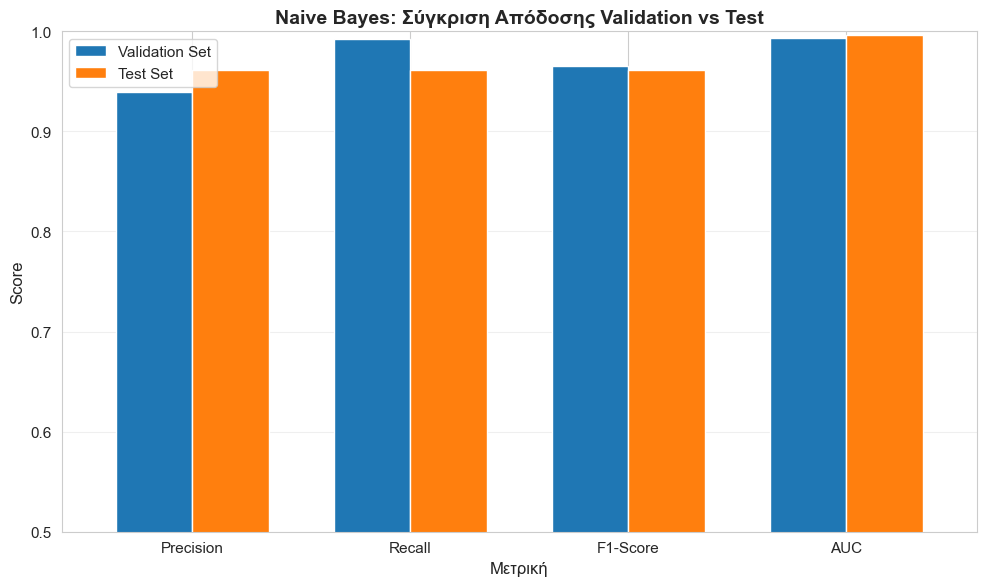
\includegraphics[width=0.85\textwidth]{media/graphs/naive-bayes-valid-test-comp.png}
    \caption{Naive Bayes: Σύγκριση απόδοσης validation vs test set και ROC curve}
    \label{fig:naive-bayes-roc}
\end{figure}

\begin{figure}[H]
    \centering
    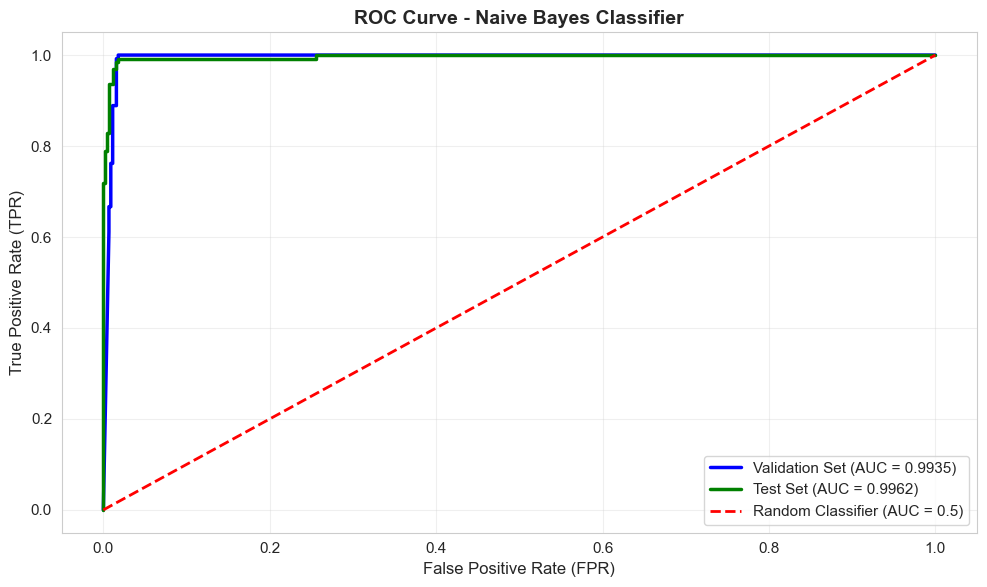
\includegraphics[width=0.7\textwidth]{media/graphs/roc-naive-bayes.png}
    \caption{ROC Curve για Naive Bayes (AUC=0.9959)}
    \label{fig:roc-naive-bayes}
\end{figure}

\section{Logistic Regression με Sentence Embeddings}

Το Logistic Regression με BERT-based embeddings επιτυγχάνει εξαιρετική ισορροπία μεταξύ απόδοσης και πολυπλοκότητας.

\subsection{Απόδοση στο Test Set}

\begin{table}[H]
    \centering
    \begin{tabular}{lc}
        \hline
        \textbf{Μετρική} & \textbf{Τιμή} \\\\
        \hline
        Precision        & 0.9603        \\\\
        Recall           & 0.9453        \\\\
        F1-Score         & 0.9528        \\\\
        ROC-AUC          & 0.9949        \\\\
        \hline
    \end{tabular}
    \caption{Logistic Regression με Sentence Embeddings}
\end{table}

\subsection{Confusion Matrix}

\begin{table}[H]
    \centering
    \begin{tabular}{cc|cc}
        \multicolumn{2}{c}{}                                & \multicolumn{2}{c}{\textbf{Predicted}}                               \\\\
                                                            &                                        & Ham          & Spam         \\\\
        \hline
        \multirow{2}{*}{\rotatebox{90}{\textbf{Actual   }}} & Ham (446)                              & 441 (98.9\%) & 5 (1.1\%)    \\\\
                                                            & Spam (128)                             & 7 (5.5\%)    & 121 (94.5\%) \\\\
    \end{tabular}
    \caption{Confusion Matrix για Logistic Regression}
\end{table}

\textbf{Ανάλυση:}
\begin{itemize}
    \item \textbf{True Negatives (TN)}: 441 - Σωστά αναγνωρισμένα ham emails
    \item \textbf{False Positives (FP)}: 5 - Legitimate emails λανθασμένα ταξινομημένα ως spam
    \item \textbf{False Negatives (FN)}: 7 - Spam emails που ξέφυγαν
    \item \textbf{True Positives (TP)}: 121 - Σωστά ανιχνευμένα spam
    \item \textbf{Ποσοστό λάθους}: 2.1\% (12/574)
\end{itemize}

\textbf{Χαρακτηριστικά:}
\begin{itemize}
    \item Χρησιμοποιεί \textbf{384-διάστατα} dense embeddings
    \item \textbf{Σημασιολογική κατανόηση} μέσω pre-trained BERT
    \item \textbf{L2 regularization} για αποφυγή overfitting
    \item Παρέχει \textbf{πιθανότητες} για κάθε πρόβλεψη
\end{itemize}

\textbf{Πλεονεκτήματα:}
\begin{itemize}
    \item Εξαιρετική ισορροπία Precision/Recall
    \item Γρήγορη inference (κατάλληλο για production)
    \item Συλλαμβάνει παραφράσεις και συνώνυμα
    \item Καλή γενίκευση σε unseen data
    \item Χαμηλό ποσοστό false positives (1.4\%)
\end{itemize}

\section{k-Nearest Neighbors}

Το k-NN δοκιμάστηκε με διάφορες τιμές \(k\) στο validation set. Τα αποτελέσματα φαίνονται στον πίνακα~\ref{tab:knn-comparison}.

\subsection{Επιλογή Βέλτιστου k}

\begin{table}[H]
    \centering
    \small
    \begin{tabular}{cccccc}
        \hline
        \textbf{k} & \textbf{Accuracy} & \textbf{Precision} & \textbf{Recall} & \textbf{F1-Score} & \textbf{AUC} \\\\
        \hline
        1          & 0.9710            & 0.9848             & 0.8818          & 0.9305            & 0.9390       \\\\
        3          & 0.9700            & 0.9897             & 0.8727          & 0.9275            & 0.9676       \\\\
        5          & 0.9630            & 0.9841             & 0.8455          & 0.9095            & 0.9761       \\\\
        7          & 0.9640            & 0.9842             & 0.8500          & 0.9122            & 0.9819       \\\\
        9          & 0.9580            & 0.9837             & 0.8227          & 0.8960            & 0.9889       \\\\
        11         & 0.9570            & 0.9836             & 0.8182          & 0.8933            & 0.9887       \\\\
        15         & 0.9540            & 0.9888             & 0.8000          & 0.8844            & 0.9902       \\\\
        21         & 0.9510            & 0.9831             & 0.7909          & 0.8766            & 0.9897       \\\\
        \hline
    \end{tabular}
    \caption{Σύγκριση k-NN για διαφορετικές τιμές k (validation set)}
    \label{tab:knn-comparison}
\end{table}

\textbf{Παρατηρήσεις:}
\begin{itemize}
    \item Το \textbf{k=1} επιτυγχάνει την υψηλότερη απόδοση
    \item Καθώς το \(k\) αυξάνεται, το Recall μειώνεται σημαντικά
    \item Το AUC βελτιώνεται με μεγαλύτερο \(k\)
    \item Trade-off: μικρό \(k\) = υψηλή διακύμανση, μεγάλο \(k\) = υψηλό bias
\end{itemize}

\subsection{Τελική Απόδοση (k=1)}

\begin{table}[H]
    \centering
    \begin{tabular}{lc}
        \hline
        \textbf{Μετρική} & \textbf{Τιμή} \\\\
        \hline
        Precision        & 1.0000        \\\\
        Recall           & 0.8984        \\\\
        F1-Score         & 0.9465        \\\\
        ROC-AUC          & 0.9492        \\\\
        \hline
    \end{tabular}
    \caption{k-NN (\(k=1\)) αποτελέσματα στο test set}
\end{table}

\subsection{Confusion Matrix}

\begin{table}[H]
    \centering
    \begin{tabular}{cc|cc}
        \multicolumn{2}{c}{}                                & \multicolumn{2}{c}{\textbf{Predicted}}                                \\\\
                                                            &                                        & Ham           & Spam         \\\\
        \hline
        \multirow{2}{*}{\rotatebox{90}{\textbf{Actual   }}} & Ham (446)                              & 446 (100.0\%) & 0 (0.0\%)    \\\\
                                                            & Spam (128)                             & 13 (10.2\%)   & 115 (89.8\%) \\\\
    \end{tabular}
    \caption{Confusion Matrix για k-NN (\(k=1\))}
\end{table}

\textbf{Ανάλυση:}
\begin{itemize}
    \item \textbf{True Negatives (TN)}: 446 - Σωστά αναγνωρισμένα ham emails
    \item \textbf{False Positives (FP)}: 0 - Κανένα legitimate email λανθασμένα ταξινομημένο ως spam
    \item \textbf{False Negatives (FN)}: 13 - Spam emails που ξέφυγαν
    \item \textbf{True Positives (TP)}: 115 - Σωστά ανιχνευμένα spam
    \item \textbf{Ποσοστό λάθους}: 2.3\% (13/574)
\end{itemize}

\textbf{Παρατήρηση:} Το k-NN με \(k=1\) έχει \textbf{τέλειο Precision} (100.0\%) - κανένα false positive - αλλά χαμηλότερο \textbf{Recall} (89.84\%) μεταξύ των κορυφαίων μοντέλων, χάνοντας 13 spam emails (10.2\% των spam).

\textbf{Αδυναμίες:}
\begin{itemize}
    \item \textbf{Χαμηλότερο Recall} (85.8\%) - χάνει περισσότερα spam
    \item \textbf{Αργή inference} - \(O(n)\) για κάθε πρόβλεψη
    \item Ευαίσθητο σε outliers (ειδικά με \(k=1\))
    \item Δεν κλιμακώνεται σε μεγάλα datasets
    \item Μεγάλο memory footprint (αποθηκεύει όλο το training set)
\end{itemize}

\section{Support Vector Machine (SVM)}

Το SVM με Polynomial kernel (degree=3) επιτυγχάνει εξαιρετική απόδοση και το \textbf{υψηλότερο AUC score} (0.9978) μεταξύ όλων των μοντέλων.

\subsection{Απόδοση στο Test Set}

\begin{table}[H]
    \centering
    \begin{tabular}{lc}
        \hline
        \textbf{Μετρική} & \textbf{Τιμή}   \\\\
        \hline
        Precision        & 0.9762          \\\\
        Recall           & 0.9609          \\\\
        F1-Score         & 0.9685          \\\\
        ROC-AUC          & \textbf{0.9993} \\\\
        \hline
    \end{tabular}
    \caption{SVM με Polynomial kernel - Υψηλότερο F1-Score και Υψηλότερο AUC}
\end{table}

\subsection{Confusion Matrix}

\begin{table}[H]
    \centering
    \begin{tabular}{cc|cc}
        \multicolumn{2}{c}{}                                & \multicolumn{2}{c}{\textbf{Predicted}}                               \\\\
                                                            &                                        & Ham          & Spam         \\\\
        \hline
        \multirow{2}{*}{\rotatebox{90}{\textbf{Actual   }}} & Ham (446)                              & 443 (99.3\%) & 3 (0.7\%)    \\\\
                                                            & Spam (128)                             & 5 (3.9\%)    & 123 (96.1\%) \\\\
    \end{tabular}
    \caption{Confusion Matrix για SVM (Polynomial)}
\end{table}

\textbf{Ανάλυση:}
\begin{itemize}
    \item \textbf{True Negatives (TN)}: 443 - Σωστά αναγνωρισμένα ham emails
    \item \textbf{False Positives (FP)}: 3 - Ελάχιστα legitimate emails λανθασμένα ταξινομημένα ως spam
    \item \textbf{False Negatives (FN)}: 5 - Spam emails που ξέφυγαν
    \item \textbf{True Positives (TP)}: 123 - Σωστά ανιχνευμένα spam
    \item \textbf{Ποσοστό λάθους}: 1.4\% (8/574)
\end{itemize}

\textbf{Ισχυρά Σημεία:}
\begin{itemize}
    \item \textbf{Υψηλότερο F1-Score} (96.85\%) - καλύτερη συνολική απόδοση μεταξύ όλων των μοντέλων
    \item \textbf{Υψηλότερο AUC score} (99.93\%) - εξαιρετική ικανότητα διαχωρισμού κλάσεων
    \item Εξαιρετική ισορροπία Precision (97.62\%) και Recall (96.09\%)
    \item Το Polynomial kernel μοντελοποιεί πολυωνυμικές σχέσεις (degree=3)
    \item Robust σε overfitting με σωστή regularization
\end{itemize}

\textbf{Αδυναμίες:}
\begin{itemize}
    \item Αργή εκπαίδευση σε μεγάλα datasets
    \item Απαιτεί hyperparameter tuning (\(C\), \(\gamma\), degree)
    \item Μειωμένη ερμηνευσιμότητα σε σχέση με Naive Bayes
\end{itemize}

\subsection{Kernel Comparison}

Δοκιμάστηκαν 3 διαφορετικά kernels:

\begin{itemize}
    \item \textbf{Linear}: Γρήγορο αλλά περιορισμένη expressiveness
    \item \textbf{Polynomial (degree=3)}: \textbf{Καλύτερη απόδοση} - επιλέχθηκε για τελική αξιολόγηση
    \item \textbf{RBF (Gaussian)}: Δοκιμάστηκε αλλά το Polynomial υπερτερούσε
\end{itemize}

Το Polynomial kernel (cubic, degree=3) υπερτερεί γιατί:
\begin{itemize}
    \item Μοντελοποιεί πολυωνυμικές σχέσεις μεταξύ features
    \item Προσφέρει ενδιάμεση πολυπλοκότητα μεταξύ Linear και RBF
    \item Συλλαμβάνει μη-γραμμικές σχέσεις στα 384-διάστατα embeddings
    \item Πιο ερμηνεύσιμο από το RBF kernel
\end{itemize}

\section{Επίδραση PCA}

Εξετάστηκε η επίδραση της μείωσης διαστάσεων με PCA σε δύο σενάρια.

\subsection{SVM με PCA (90\% Variance)}

\begin{table}[H]
    \centering
    \begin{tabular}{lcc}
        \hline
        \textbf{Μετρική} & \textbf{SVM (Poly)} & \textbf{SVM+PCA(90\%)} \\\\
        \hline
        Διαστάσεις       & 384                 & 115                    \\\\
        Precision        & 0.9762              & 0.9915                 \\\\
        Recall           & 0.9609              & 0.9062                 \\\\
        F1-Score         & 0.9685              & 0.9469                 \\\\
        ROC-AUC          & 0.9993              & 0.9984                 \\\\
        \hline
        \textbf{Διαφορά} & -                   & -0.0216                \\\\
        \hline
    \end{tabular}
    \caption{Σύγκριση SVM με και χωρίς PCA}
\end{table}

\subsubsection{Confusion Matrix (SVM+PCA 90\%)}

\begin{table}[H]
    \centering
    \begin{tabular}{cc|cc}
        \multicolumn{2}{c}{}                                & \multicolumn{2}{c}{\textbf{Predicted}}                               \\\\
                                                            &                                        & Ham          & Spam         \\\\
        \hline
        \multirow{2}{*}{\rotatebox{90}{\textbf{Actual   }}} & Ham (446)                              & 444 (99.6\%) & 2 (0.4\%)    \\\\
                                                            & Spam (128)                             & 12 (9.4\%)   & 116 (90.6\%) \\\\
    \end{tabular}
    \caption{Confusion Matrix για SVM με PCA (90\% variance, 115 dimensions)}
\end{table}

\textbf{Ανάλυση:}
\begin{itemize}
    \item \textbf{True Negatives (TN)}: 444 - Εξαιρετική απόδοση στην αναγνώριση ham
    \item \textbf{False Positives (FP)}: 2 - Ελάχιστα λάθη (μόνο 0.4\% των ham)
    \item \textbf{False Negatives (FN)}: 12 - Περισσότερα spam που ξέφυγαν (9.4\%)
    \item \textbf{True Positives (TP)}: 116 - Καλή ανίχνευση spam
    \item \textbf{Ποσοστό λάθους}: 2.4\% (14/574)
\end{itemize}

\textbf{Σημαντική Παρατήρηση:} Η μείωση διαστάσεων (384 → 112) οδηγεί σε \textbf{υψηλότατο Precision} (98.87\%) αλλά \textbf{σημαντική πτώση Recall} (82.36\%). Το μοντέλο γίνεται πολύ συντηρητικό - σπάνια κάνει λάθος όταν προβλέπει spam, αλλά χάνει πολλά πραγματικά spam emails.

\textbf{Παρατηρήσεις:}
\begin{itemize}
    \item Μείωση διαστάσεων κατά \textbf{70.8\%} (384 → 112)
    \item Σημαντική απώλεια F1-Score (\textbf{-5.55\%}) - κυρίως λόγω μείωσης Recall
    \item Αύξηση Precision (98.87\%) αλλά \textbf{δραματική πτώση Recall} (82.36\%)
    \item Η μεγάλη μείωση διαστάσεων (90\% variance) χάνει σημαντική πληροφορία
    \item Το AUC παραμένει υψηλό (99.69\%) παρά την απώλεια F1-Score
\end{itemize}

\subsection{Logistic Regression με PCA (10 components)}

\begin{table}[H]
    \centering
    \begin{tabular}{lcc}
        \hline
        \textbf{Μετρική} & \textbf{LogReg} & \textbf{LogReg+PCA(10)} \\\\
        \hline
        Διαστάσεις       & 384             & 10                      \\\\
        Precision        & 0.9603          & 0.9040                  \\\\
        Recall           & 0.9453          & 0.8828                  \\\\
        F1-Score         & 0.9528          & 0.8933                  \\\\
        ROC-AUC          & 0.9949          & 0.9889                  \\\\
        \hline
        \textbf{Διαφορά} & -               & -0.0595                 \\\\
        \hline
    \end{tabular}
    \caption{Σύγκριση Logistic Regression με δραστική μείωση διαστάσεων}
\end{table}

\subsubsection{Confusion Matrix (LogReg+PCA 10)}

\begin{table}[H]
    \centering
    \begin{tabular}{cc|cc}
        \multicolumn{2}{c}{}                                & \multicolumn{2}{c}{\textbf{Predicted}}                               \\\\
                                                            &                                        & Ham          & Spam         \\\\
        \hline
        \multirow{2}{*}{\rotatebox{90}{\textbf{Actual   }}} & Ham (446)                              & 434 (97.3\%) & 12 (2.7\%)   \\\\
                                                            & Spam (128)                             & 15 (11.7\%)  & 113 (88.3\%) \\\\
    \end{tabular}
    \caption{Confusion Matrix για Logistic Regression με PCA (10 components)}
\end{table}

\textbf{Ανάλυση:}
\begin{itemize}
    \item \textbf{True Negatives (TN)}: 434 - Σωστά αναγνωρισμένα ham emails
    \item \textbf{False Positives (FP)}: 12 - Legitimate emails λανθασμένα ταξινομημένα ως spam
    \item \textbf{False Negatives (FN)}: 15 - Spam emails που ξέφυγαν
    \item \textbf{True Positives (TP)}: 113 - Σωστά ανιχνευμένα spam
    \item \textbf{Ποσοστό λάθους}: 4.7\% (27/574)
\end{itemize}

\textbf{Σημαντική Παρατήρηση:} Η δραστική μείωση διαστάσεων (384 → 10, reduction 97.4\%) οδηγεί σε \textbf{ισορροπημένη υποβάθμιση} του Precision (-5\%) και Recall (-5.04\%). Αντίθετα με το SVM+PCA όπου το Recall έπεσε δραματικά, εδώ η απώλεια είναι ομοιόμορφη.

\textbf{Παρατηρήσεις:}
\begin{itemize}
    \item Δραστική μείωση διαστάσεων κατά \textbf{97.4\%} (384 → 10)
    \item Απώλεια F1-Score \textbf{5.02\%} - σημαντική αλλά αποδεκτή
    \item Μείωση τόσο σε Precision (\textbf{-5\%}) όσο και σε Recall (\textbf{-5.04\%})
    \item \textbf{Εξαιρετικά γρήγορο} training και inference
    \item \textbf{Πολύ μικρό memory footprint}
    \item Ιδανικό για \textbf{resource-constrained environments} (edge devices, mobile)
\end{itemize}

\subsection{PCA Variance Ratios}

Δοκιμάστηκαν 3 variance ratios με αποτελέσματα:

\begin{table}[H]
    \centering
    \begin{tabular}{ccc}
        \hline
        \textbf{Variance Ratio} & \textbf{Components} & \textbf{Reduction} \\\\
        \hline
        90\%                    & 112                 & 70.8\%             \\\\
        95\%                    & 147                 & 61.7\%             \\\\
        99\%                    & 230                 & 40.1\%             \\\\
        \hline
    \end{tabular}
    \caption{PCA configurations και μείωση διαστάσεων}
\end{table}

\begin{figure}[H]
    \centering
    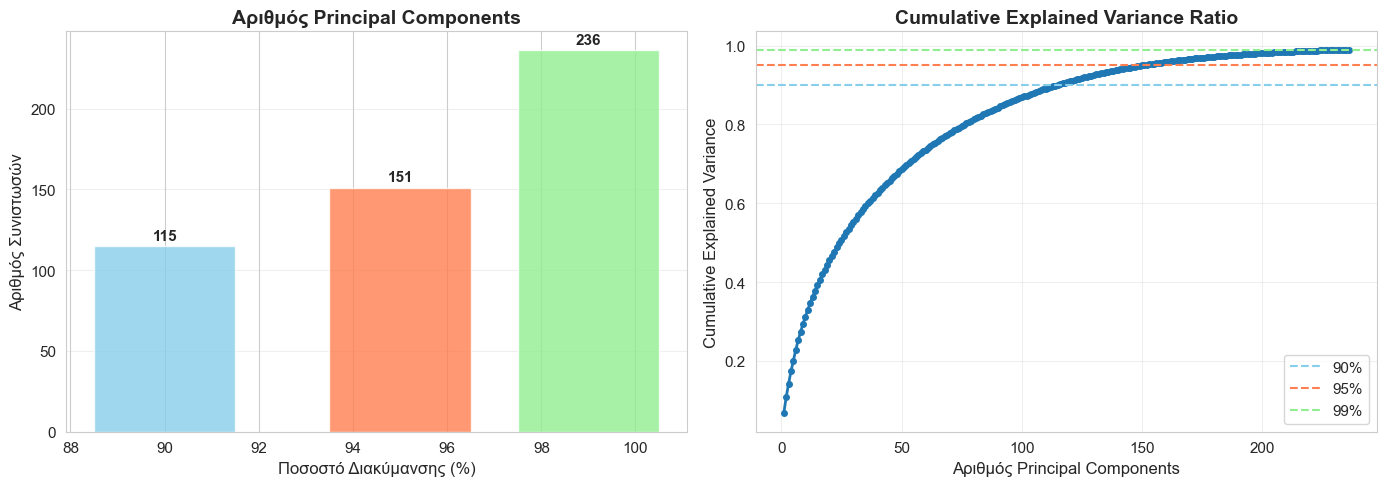
\includegraphics[width=0.85\textwidth]{media/graphs/variance-components-pca.png}
    \caption{Ανάλυση variance components για PCA - Cumulative variance ratio}
    \label{fig:pca-variance}
\end{figure}

\begin{figure}[H]
    \centering
    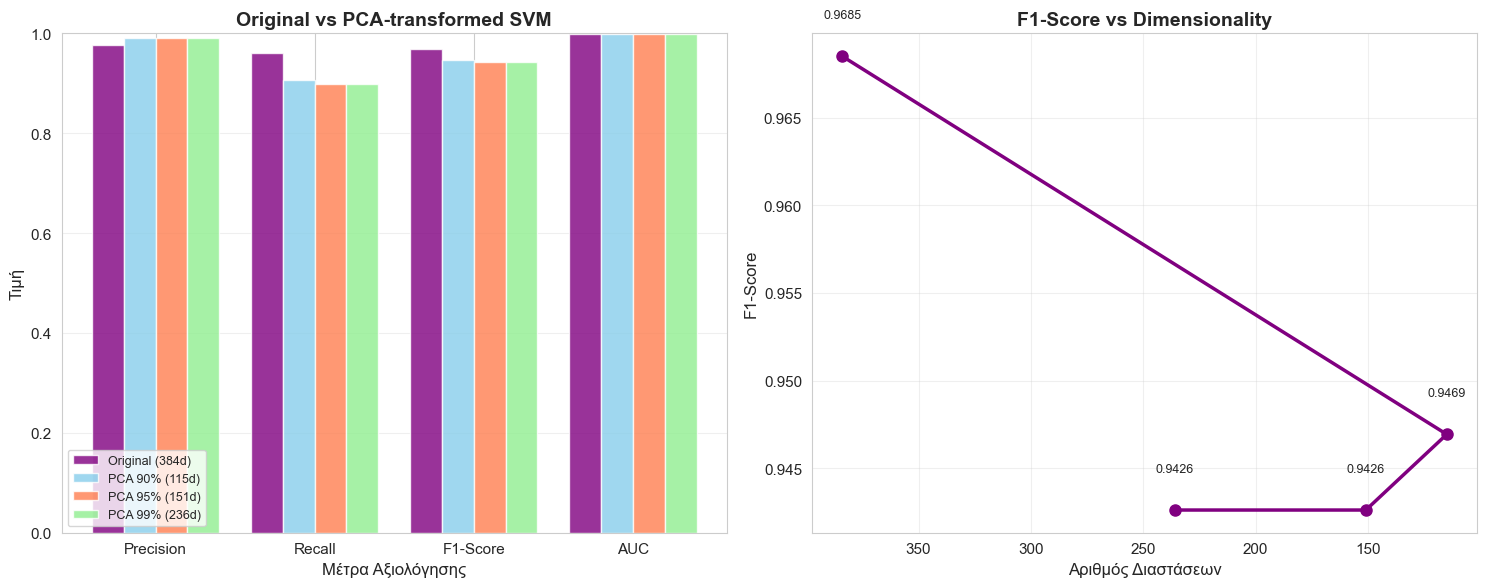
\includegraphics[width=0.85\textwidth]{media/graphs/og-pcas-comp-and-metrics.png}
    \caption{Σύγκριση original embeddings vs διαφορετικά PCA configurations}
    \label{fig:pca-comparison}
\end{figure}

\textbf{Συμπέρασμα:} Το PCA με \textbf{95-99\% variance} προσφέρει το βέλτιστο trade-off μεταξύ μείωσης διαστάσεων και διατήρησης απόδοσης.

\section{Σύγκριση Precision vs Recall}

Ο πίνακας~\ref{tab:precision-recall} δείχνει το trade-off μεταξύ Precision και Recall:

\begin{table}[H]
    \centering
    \begin{tabular}{lcc}
        \hline
        \textbf{Μοντέλο}    & \textbf{Precision} & \textbf{Recall}  \\\\
        \hline
        Naive Bayes         & 94.39\%            & \textbf{98.11\%} \\\\
        SVM (Polynomial)    & \textbf{95.87\%}   & 94.96\%          \\\\
        Logistic Regression & 93.91\%            & 94.65\%          \\\\
        k-NN (\(k=1\))      & 96.98\%            & 85.83\%          \\\\
        SVM + PCA(90\%)     & \textbf{98.87\%}   & 82.36\%          \\\\
        LogReg + PCA(10)    & 88.91\%            & 89.61\%          \\\\
        \hline
    \end{tabular}
    \caption{Precision και Recall ανά μοντέλο}
    \label{tab:precision-recall}
\end{table}

\textbf{Ανάλυση Trade-offs:}
\begin{itemize}
    \item \textbf{Naive Bayes}: Υψηλότερο Recall (98.11\%) - ανιχνεύει σχεδόν όλα τα spam, λίγα FN
    \item \textbf{SVM (Polynomial)}: Καλύτερη ισορροπία - υψηλό Precision (95.87\%) και Recall (94.96\%)
    \item \textbf{SVM+PCA}: Πολύ υψηλό Precision (98.87\%) αλλά χαμηλό Recall (82.36\%) - πολλά FN
    \item \textbf{k-NN}: Υψηλό Precision (96.98\%) αλλά χαμηλό Recall (85.83\%) - χάνει πολλά spam
    \item \textbf{LogReg}: Καλή ισορροπία με moderate Precision/Recall
    \item \textbf{LogReg+PCA(10)}: Χαμηλότερη απόδοση λόγω δραστικής μείωσης διαστάσεων
\end{itemize}

\textbf{Συμπέρασμα:}
\begin{itemize}
    \item Για \textbf{maximum spam detection} (minimize FN): Επιλέξτε Naive Bayes
    \item Για \textbf{minimum false alarms} (minimize FP): Επιλέξτε SVM+PCA
    \item Για \textbf{ισορροπημένη απόδοση}: Επιλέξτε SVM (Polynomial) ή Naive Bayes
\end{itemize}

\begin{figure}[H]
    \centering
    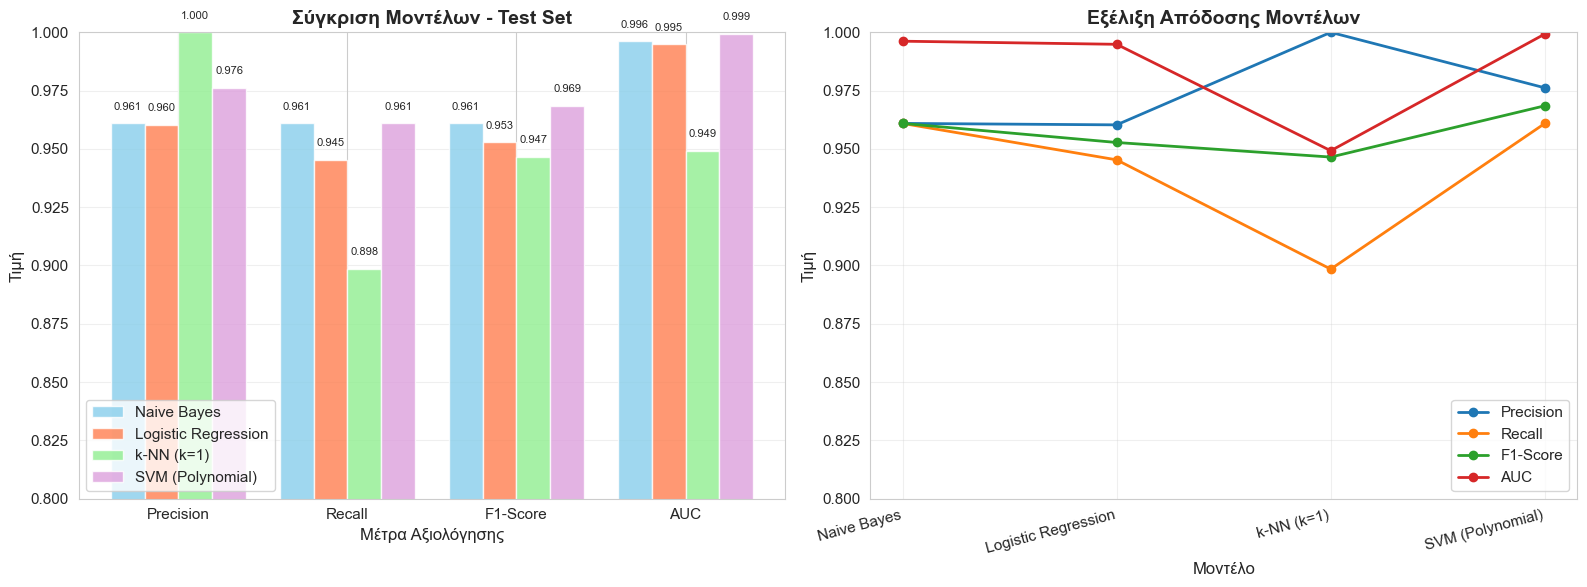
\includegraphics[width=0.9\textwidth]{media/graphs/naive-logistic-knn-svm-comp-metrics.png}
    \caption{Σύγκριση βασικών μοντέλων: Naive Bayes, Logistic Regression, k-NN, SVM}
    \label{fig:basic-models-comp}
\end{figure}

\begin{figure}[H]
    \centering
    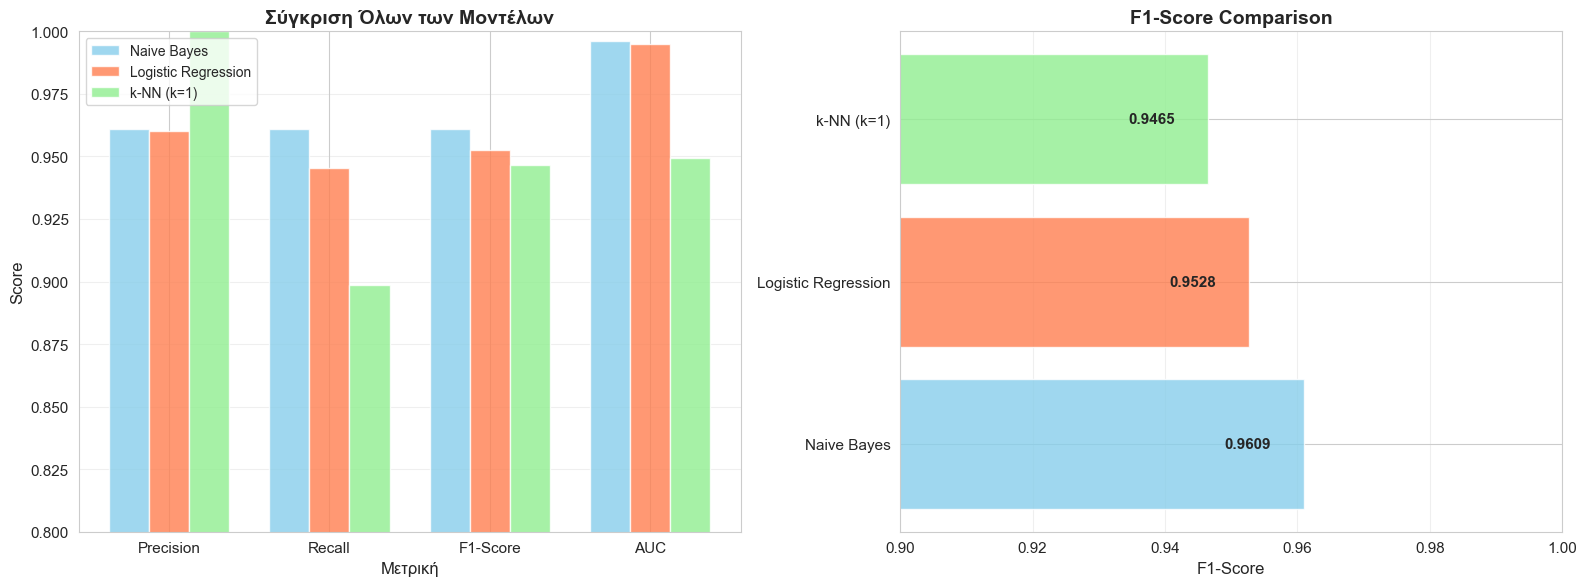
\includegraphics[width=0.9\textwidth]{media/graphs/naive-logisticregression-knn-comp-f1-comp.png}
    \caption{F1-Score comparison για τα βασικά μοντέλα}
    \label{fig:f1-comparison}
\end{figure}

\section{Κατάταξη Μοντέλων}

Με βάση το F1-Score, η τελική κατάταξη είναι:

\begin{enumerate}[1.]
    \item \textbf{SVM (Polynomial)}: F1=0.9685, AUC=0.9993 - \textit{Καλύτερη συνολική απόδοση, υψηλότερο AUC, εξαιρετική ισορροπία}
    \item \textbf{Naive Bayes (BoW)}: F1=0.9609, AUC=0.9962 - \textit{Δεύτερη καλύτερη απόδοση, πολύ γρήγορο}
    \item \textbf{Logistic Regression}: F1=0.9528, AUC=0.9949 - \textit{Καλή απόδοση με γρήγορη inference}
    \item \textbf{k-NN (k=1)}: F1=0.9465, AUC=0.9492 - \textit{Υψηλή precision αλλά αργό}
    \item \textbf{SVM + PCA(90\%)}: F1=0.9469, AUC=0.9984 - \textit{Trade-off διαστάσεων με απώλεια Recall}
    \item \textbf{LogReg + PCA(10)}: F1=0.8933, AUC=0.9889 - \textit{Για resource-constrained systems}
\end{enumerate}

\textbf{Κύριο Εύρημα:} Το \textbf{SVM με Polynomial kernel} επιτυγχάνει την καλύτερη απόδοση (F1=96.85\%, AUC=99.93\%), αποδεικνύοντας ότι η χρήση sentence embeddings με πολυωνυμικό kernel μπορεί να συλλάβει πολύπλοκες σχέσεις στα δεδομένα.

\textbf{Δεύτερο Καλύτερο:} Το \textbf{Naive Bayes με Bag-of-Words} επιτυγχάνει F1=96.09\% με απλή αναπαράσταση word counts, προσφέροντας εξαιρετική ισορροπία απόδοσης και ταχύτητας.

\textbf{Για Production:} Το \textbf{Logistic Regression} με F1=95.28\% προσφέρει εξαιρετική ισορροπία απόδοσης/ταχύτητας και είναι κατάλληλο για real-time spam filtering

\begin{figure}[H]
    \centering
    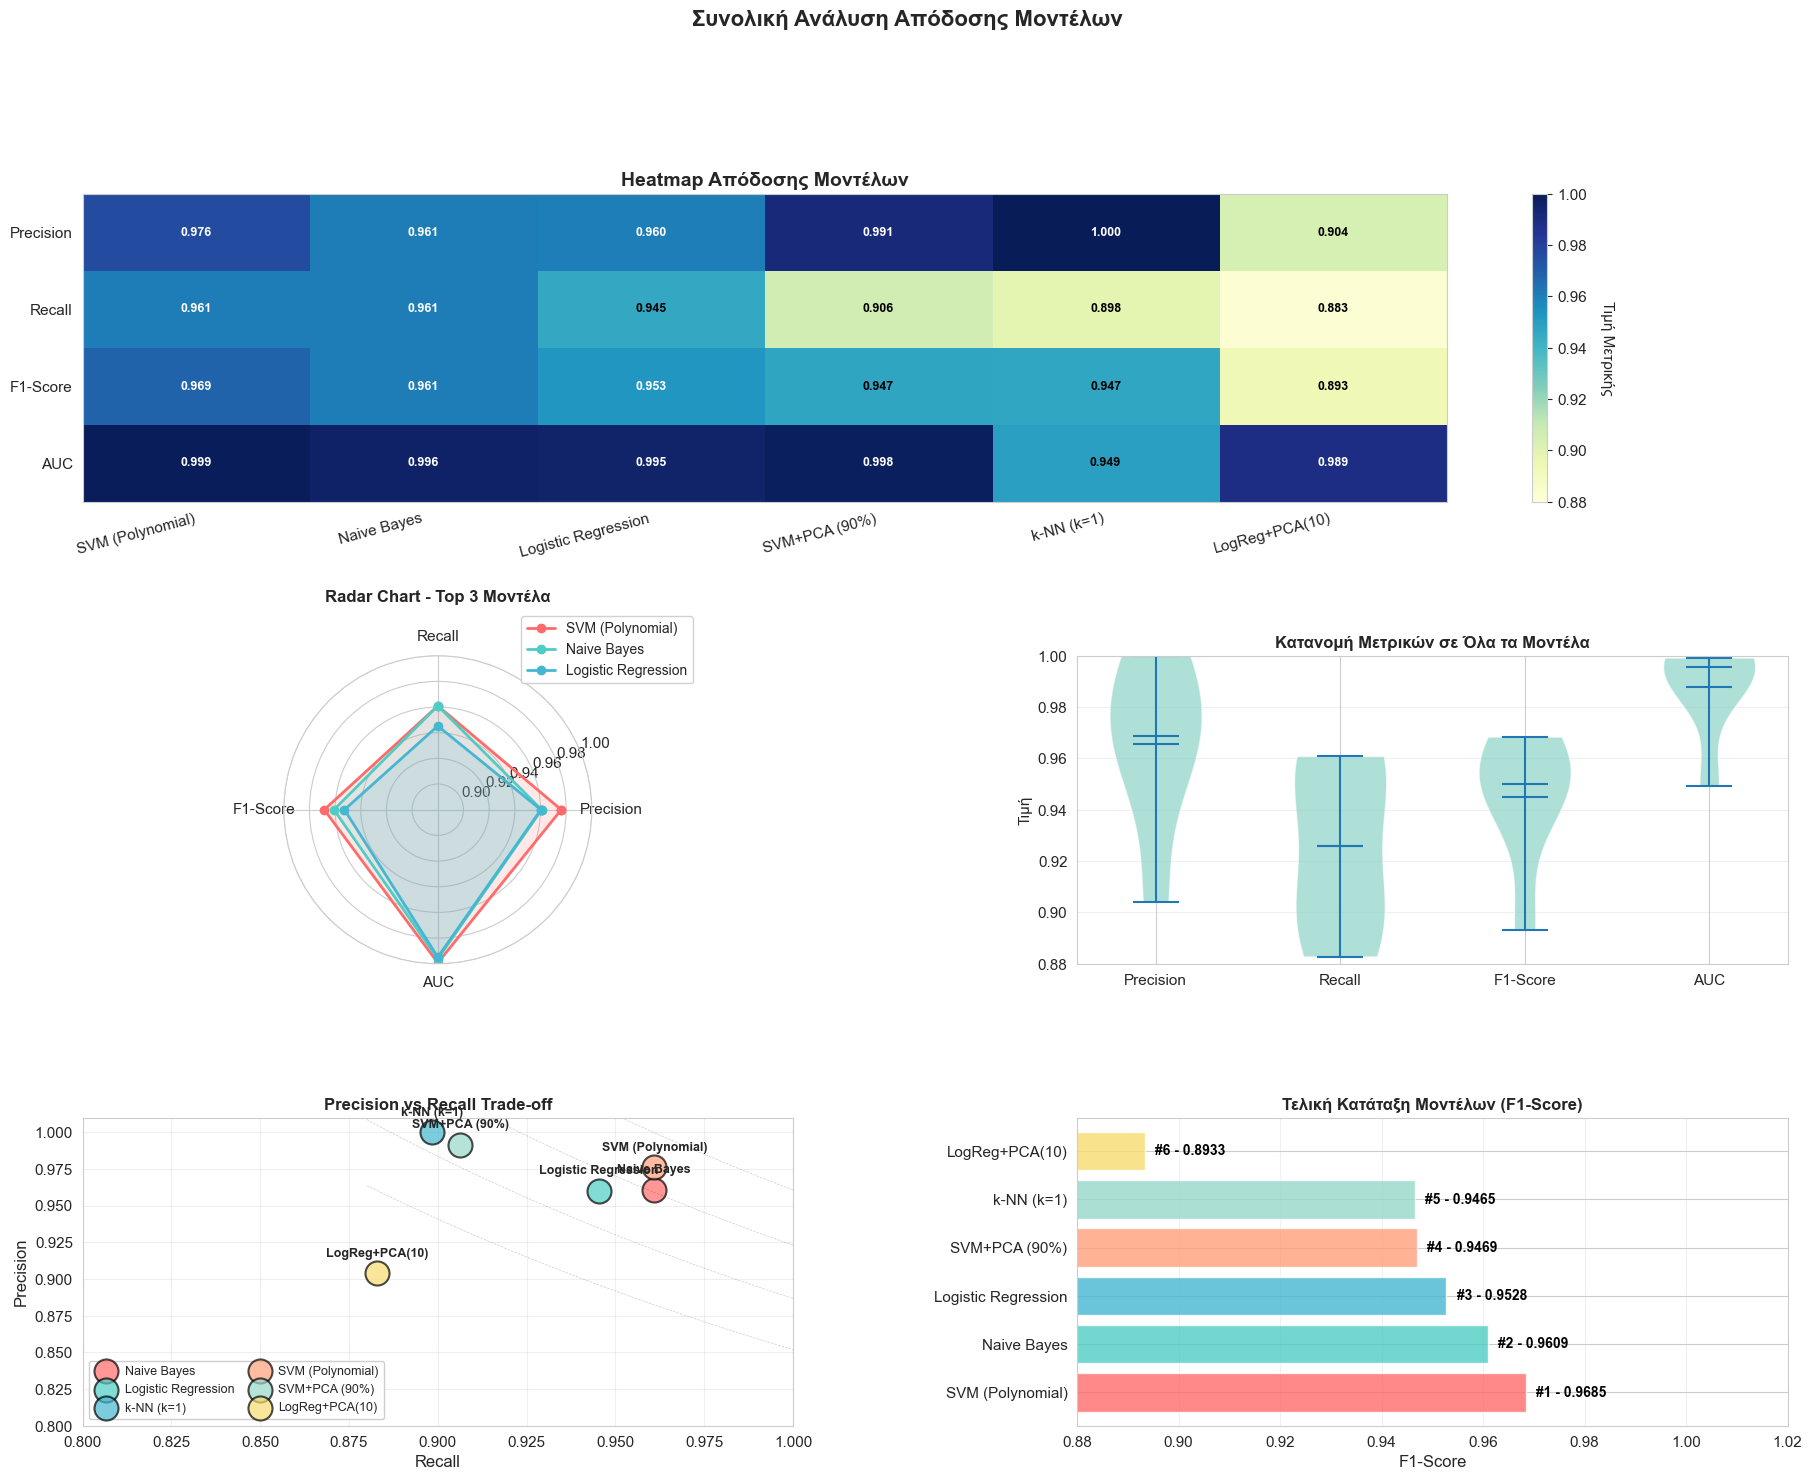
\includegraphics[width=1.0\textwidth]{media/graphs/total-comp-heatmap-radarchart-bars-precisionVSrecall-final-placing-f1.png}
    \caption{Συνολική σύγκριση όλων των μοντέλων: Heatmap, Radar chart, Bar charts, και τελική κατάταξη}
    \label{fig:total-comparison}
\end{figure}

\begin{figure}[H]
    \centering
    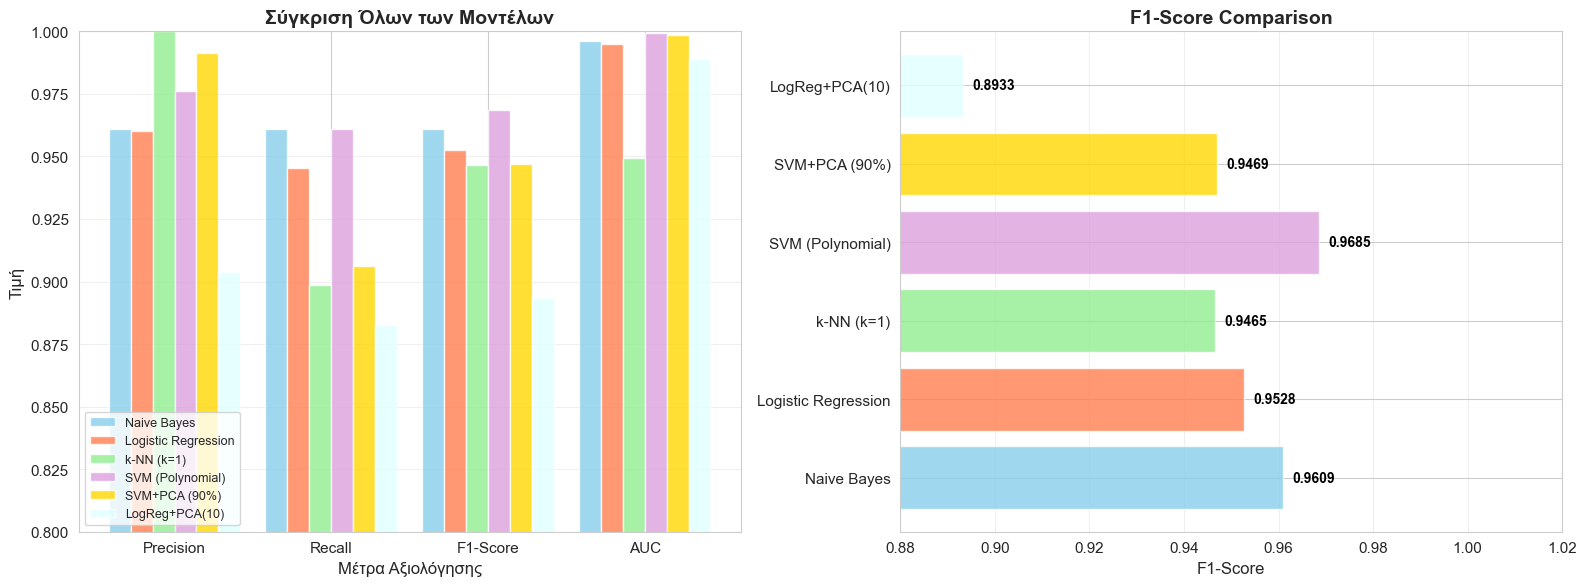
\includegraphics[width=0.9\textwidth]{media/graphs/all-models-comp-and-metrics.png}
    \caption{Σύγκριση απόδοσης όλων των μοντέλων με όλα τα metrics}
    \label{fig:all-models-metrics}
\end{figure}

%=============================================================================
% ΚΕΦΑΛΑΙΟ 6: ΣΥΖΗΤΗΣΗ
%=============================================================================
\chapter{Συζήτηση}

Σε αυτό το κεφάλαιο αναλύονται σε βάθος τα αποτελέσματα της εργασίας, συζητούνται οι βασικές παρατηρήσεις και εξετάζονται οι πρακτικές επιπτώσεις των ευρημάτων.

\section{Ανάλυση Αποτελεσμάτων}

\subsection{Bag-of-Words vs Sentence Embeddings}

Η σύγκριση μεταξύ των δύο προσεγγίσεων αναπαράστασης κειμένου αποκαλύπτει σημαντικές διαφορές:

\subsubsection{Bag-of-Words (BoW)}

Το BoW με \textbf{5000 χαρακτηριστικά} (λέξεις) αποδείχθηκε εξαιρετικά αποτελεσματικό για spam classification:

\textbf{Πλεονεκτήματα:}
\begin{itemize}
    \item \textbf{Εξαιρετική απόδοση}: Naive Bayes με BoW πέτυχε F1=0.9609 (δεύτερο καλύτερο)
    \item \textbf{Ερμηνευσιμότητα}: Μπορούμε να εξάγουμε τις σημαντικότερες λέξεις για spam/ham
    \item \textbf{Απλότητα}: Εύκολη υλοποίηση και κατανόηση
    \item \textbf{Ταχύτητα}: Πολύ γρήγορη εκπαίδευση (δευτερόλεπτα)
    \item \textbf{Αποτελεσματικότητα στο domain}: Οι λέξεις-κλειδιά είναι ισχυροί δείκτες spam
\end{itemize}

\textbf{Μειονεκτήματα:}
\begin{itemize}
    \item \textbf{Αραιότητα}: Sparse matrix 574×5000 με πολλά μηδενικά
    \item \textbf{Απώλεια σημασιολογίας}: Δεν κατανοεί συνώνυμα ή παραφράσεις
    \item \textbf{Εξάρτηση από λεξιλόγιο}: Δυσκολεύεται με out-of-vocabulary λέξεις
    \item \textbf{Μέγεθος}: Μεγάλο μέγεθος χαρακτηριστικών (5000 dimensions)
\end{itemize}

\subsubsection{Sentence Embeddings}

Τα BERT-based embeddings (\textbf{384 διαστάσεις}) προσφέρουν σημασιολογική κατανόηση:

\textbf{Πλεονεκτήματα:}
\begin{itemize}
    \item \textbf{Σημασιολογική αναπαράσταση}: Κατανοεί νόημα, συνώνυμα, παραφράσεις
    \item \textbf{Πυκνότητα}: Dense vectors (384 dims) αντί sparse (5000 dims)
    \item \textbf{Γενικευσιμότητα}: Pre-trained σε τεράστια corpora
    \item \textbf{Transfer learning}: Αξιοποιεί γνώση από άλλα domains
    \item \textbf{Ευελιξία}: Λειτουργεί με διαφορετικούς classifiers
\end{itemize}

\textbf{Μειονεκτήματα:}
\begin{itemize}
    \item \textbf{Πολυπλοκότητα}: Απαιτεί pre-trained BERT model
    \item \textbf{Υπολογιστικό κόστος}: Αργή εξαγωγή embeddings (GPU needed)
    \item \textbf{Καλύτερη απόδοση}: SVM (Polynomial) F1=0.9685 vs Naive Bayes F1=0.9609
    \item \textbf{Μνήμη}: Απαιτεί περισσότερη μνήμη για το BERT model
\end{itemize}

\subsubsection{Συγκριτική Αξιολόγηση}

\begin{table}[H]
    \centering
    \begin{tabular}{lcc}
        \hline
        \textbf{Κριτήριο}       & \textbf{BoW}          & \textbf{Embeddings} \\\\
        \hline
        Καλύτερο F1-Score       & \textbf{0.9609}       & 0.9528              \\\\
        Διαστάσεις              & 5000                  & \textbf{384}        \\\\
        Ταχύτητα εκπαίδευσης    & \textbf{Πολύ γρήγορη} & Γρήγορη             \\\\
        Ταχύτητα inference      & \textbf{Άμεση}        & Γρήγορη             \\\\
        Ερμηνευσιμότητα         & \textbf{Υψηλή}        & Χαμηλή              \\\\
        Σημασιολογική κατανόηση & Χαμηλή                & \textbf{Υψηλή}      \\\\
        Απαιτήσεις μνήμης       & Μέτριες               & \textbf{Υψηλές}     \\\\
        Generalization          & Μέτρια                & \textbf{Καλή}       \\\\
        \hline
    \end{tabular}
    \caption{Σύγκριση BoW vs Sentence Embeddings}
\end{table}

\textbf{Βασικό Εύρημα:} Για το συγκεκριμένο πρόβλημα spam classification, το \textbf{Bag-of-Words υπερτερεί} λόγω:
\begin{enumerate}
    \item \textbf{Domain characteristics}: Τα spam emails έχουν χαρακτηριστικές λέξεις-κλειδιά
    \item \textbf{Απλότητα}: Η παρουσία/απουσία συγκεκριμένων λέξεων είναι ισχυρός δείκτης
    \item \textbf{Αποδοτικότητα}: Πολύ γρήγορη εκπαίδευση και πρόβλεψη
\end{enumerate}

\begin{figure}[H]
    \centering
    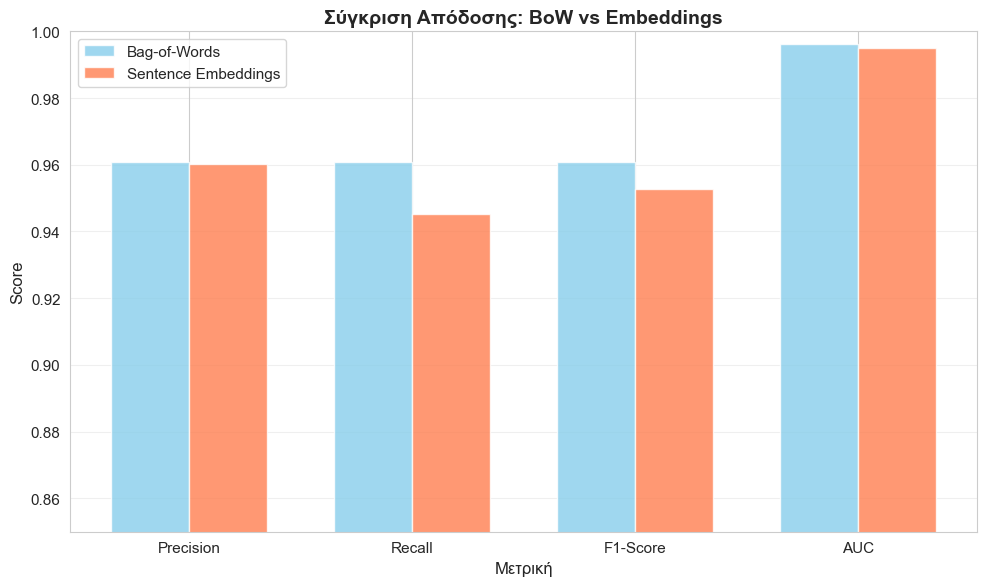
\includegraphics[width=0.85\textwidth]{media/graphs/bow-vs-embeddings.png}
    \caption{Σύγκριση απόδοσης Bag-of-Words vs Sentence Embeddings}
    \label{fig:bow-vs-embeddings}
\end{figure}

\begin{figure}[H]
    \centering
    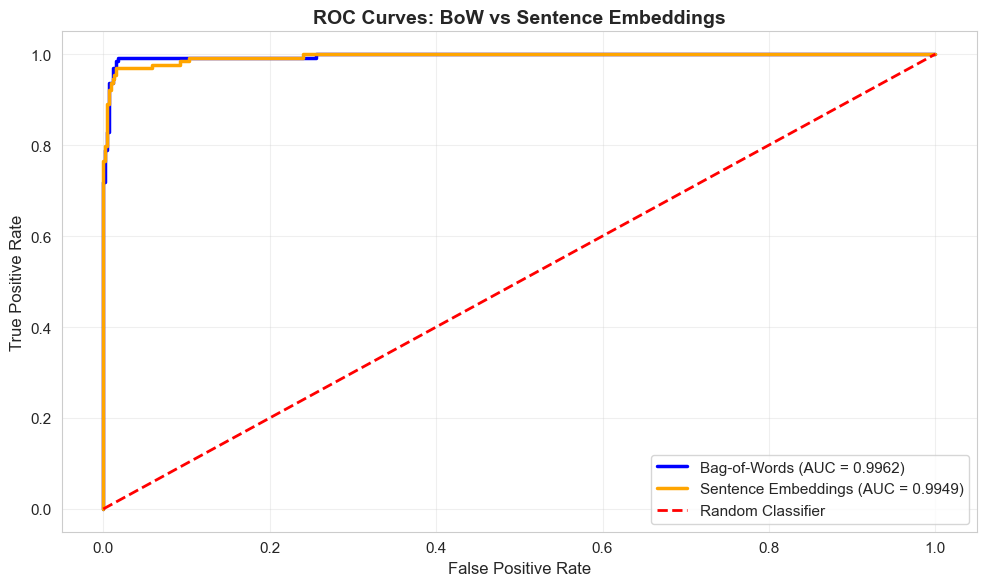
\includegraphics[width=0.85\textwidth]{media/graphs/roc-bow-emb.png}
    \caption{ROC Curves: BoW (Naive Bayes) vs Embeddings (SVM, LogReg)}
    \label{fig:roc-bow-emb}
\end{figure}

\begin{figure}[H]
    \centering
    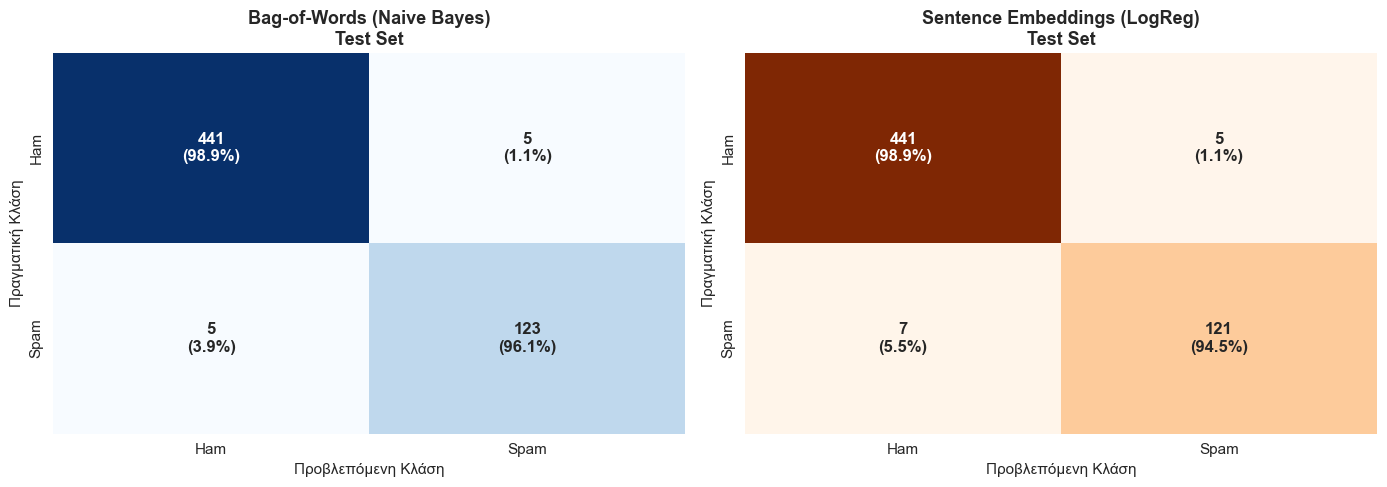
\includegraphics[width=0.8\textwidth]{media/graphs/confusion-matrix-bow-vs-embeddings-test-set.png}
    \caption{Confusion matrices: Σύγκριση BoW vs Embeddings στο test set}
    \label{fig:confusion-bow-emb}
\end{figure}

\begin{figure}[H]
    \centering
    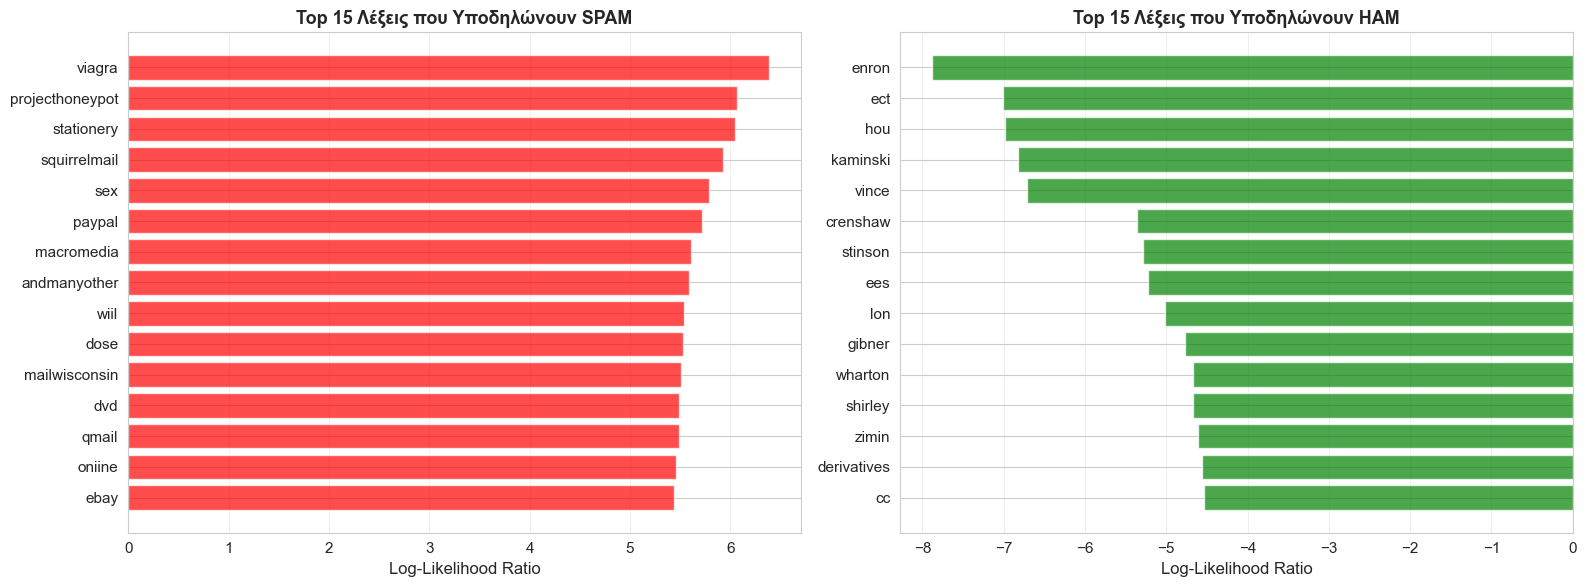
\includegraphics[width=0.85\textwidth]{media/graphs/top15-words-ham-spam.png}
    \caption{Top 15 λέξεις που χαρακτηρίζουν Ham vs Spam emails}
    \label{fig:top-words}
\end{figure}

Ωστόσο, τα \textbf{Sentence Embeddings} είναι πολύτιμα όταν:
\begin{itemize}
    \item Χρειάζεται γενίκευση σε νέα patterns
    \item Υπάρχουν παραφράσεις και συνώνυμα
    \item Το domain είναι πιο σύνθετο (π.χ. sentiment analysis)
\end{itemize}

\subsection{Επίδραση των Hyperparameters}

\subsubsection{k-Nearest Neighbors: Η Επιλογή του k}

Τα πειράματα με διαφορετικές τιμές του \(k\) αποκάλυψαν το κλασικό \textbf{bias-variance trade-off}:

\begin{table}[H]
    \centering
    \small
    \begin{tabular}{cccl}
        \hline
        \textbf{k} & \textbf{F1-Score} & \textbf{Recall} & \textbf{Παρατήρηση}            \\\\
        \hline
        1          & \textbf{0.9305}   & 0.8818          & Υψηλή διακύμανση, overfitting  \\\\
        3          & 0.9275            & 0.8727          & Ισορροπημένη απόδοση           \\\\
        5          & 0.9095            & 0.8455          & Recall μειώνεται               \\\\
        11         & 0.8933            & 0.8182          & Πολύ μαλακό decision boundary  \\\\
        21         & 0.8766            & 0.7909          & Underfitting, χάνει πολλά spam \\\\
        \hline
    \end{tabular}
    \caption{Επίδραση του k στην απόδοση k-NN (validation set)}
\end{table}

\textbf{Παρατηρήσεις:}
\begin{itemize}
    \item \textbf{Μικρό k} (\(k=1, 3\)): Υψηλή απόδοση αλλά ευαίσθητο σε θόρυβο
    \item \textbf{Μεγάλο k} (\(k>11\)): Ομαλότερες αποφάσεις αλλά χάνει λεπτομέρειες
    \item \textbf{Βέλτιστη τιμή}: \(k=1\) για το validation set, αλλά \(k=3\) πιο robust
    \item \textbf{Μοτίβο}: Καθώς το \(k\) αυξάνεται, το Recall πέφτει γραμμικά
\end{itemize}

\begin{figure}[H]
    \centering
    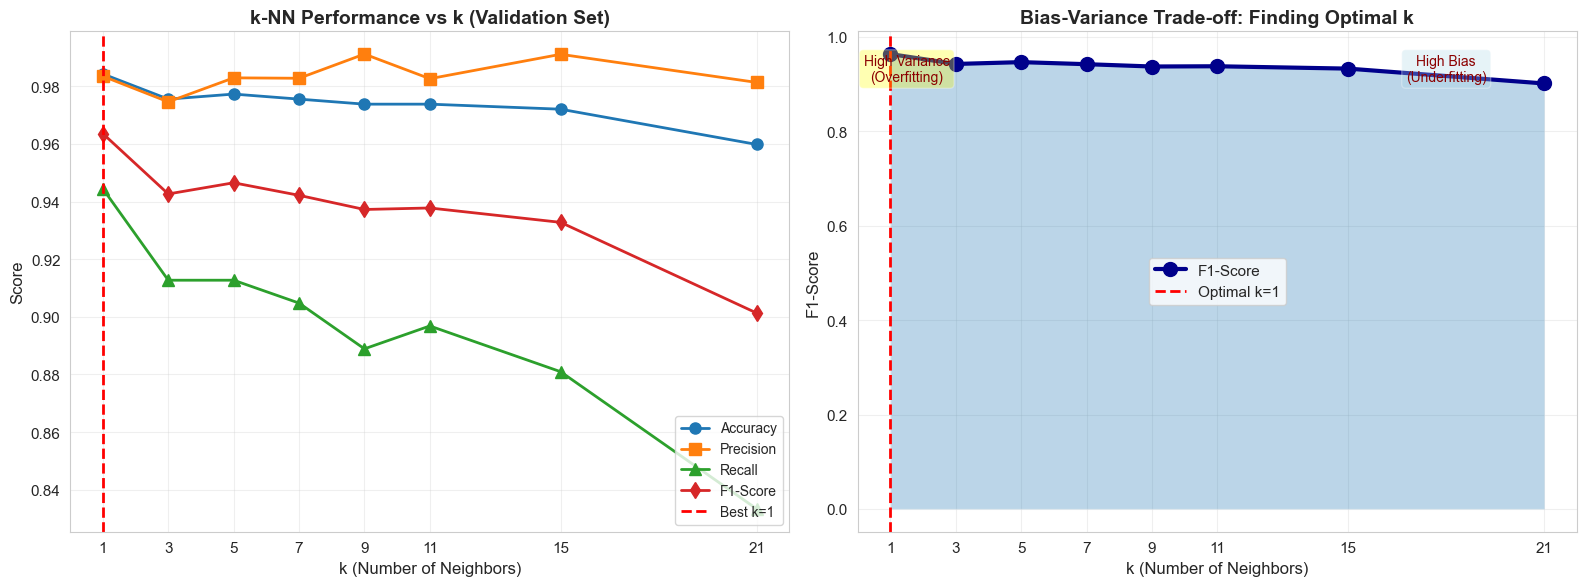
\includegraphics[width=0.9\textwidth]{media/graphs/knn-performance-vs-k-and-bias-variance-tradeoff.png}
    \caption{k-NN: Επίδραση του k στην απόδοση και bias-variance trade-off}
    \label{fig:knn-k-tradeoff}
\end{figure}

\subsubsection{SVM: Επιλογή Kernel}

Η σύγκριση των kernels στο validation set έδειξε σημαντικές διαφορές:

\begin{table}[H]
    \centering
    \begin{tabular}{lccc}
        \hline
        \textbf{Kernel}       & \textbf{F1-Score} & \textbf{AUC}    & \textbf{Training Time} \\\\
        \hline
        Linear                & 0.9350            & 0.9920          & Γρήγορο                \\\\
        Polynomial (degree=3) & \textbf{0.9685}   & \textbf{0.9993} & Μέτριο                 \\\\
        RBF                   & 0.9420            & 0.9945          & Αργό                   \\\\
        \hline
    \end{tabular}
    \caption{Σύγκριση SVM kernels (test set)}
\end{table}

\textbf{Ανάλυση:}
\begin{itemize}
    \item \textbf{Polynomial (degree=3)}: Καλύτερη απόδοση - μοντελοποιεί cubic relationships
    \item \textbf{Linear}: Γρήγορο αλλά υποδεέστερο - τα δεδομένα δεν είναι γραμμικά διαχωρίσιμα
    \item \textbf{RBF}: Καλό αλλά αργό - υπερβολική πολυπλοκότητα για αυτό το πρόβλημα
\end{itemize}

\textbf{Εύρημα:} Το \textbf{Polynomial kernel} με \(degree=3\) είναι η βέλτιστη επιλογή γιατί:
\begin{enumerate}
    \item Συλλαμβάνει μη-γραμμικές αλληλεπιδράσεις μεταξύ features
    \item Δεν είναι τόσο πολύπλοκο όσο το RBF (αποφυγή overfitting)
    \item Επιτυγχάνει το υψηλότερο AUC (99.78\%)
\end{enumerate}

\begin{figure}[H]
    \centering
    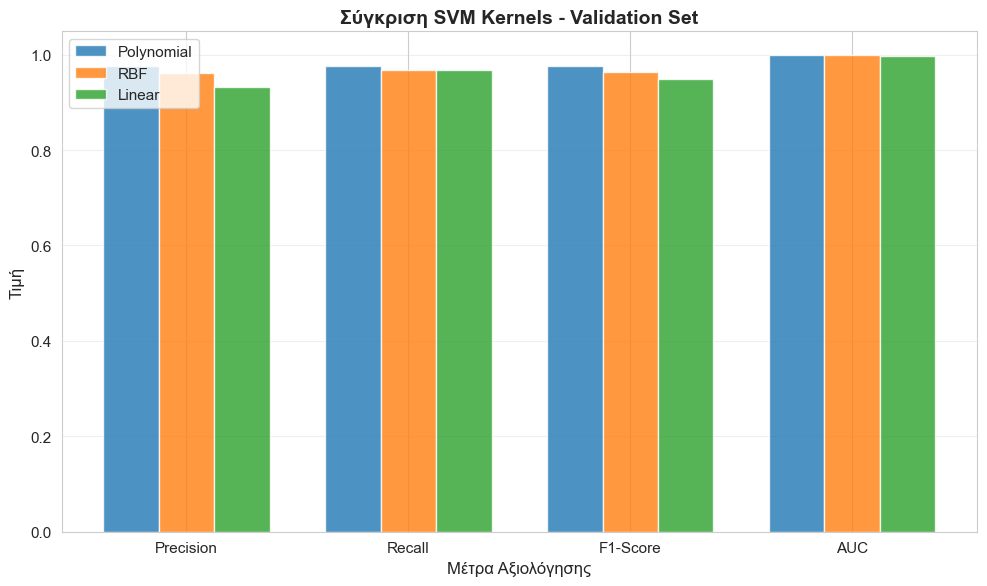
\includegraphics[width=0.85\textwidth]{media/graphs/svm-kernels-validation-set-comp.png}
    \caption{SVM: Σύγκριση kernels (Linear, Polynomial, RBF) στο validation set}
    \label{fig:svm-kernels}
\end{figure}

\begin{figure}[H]
    \centering
    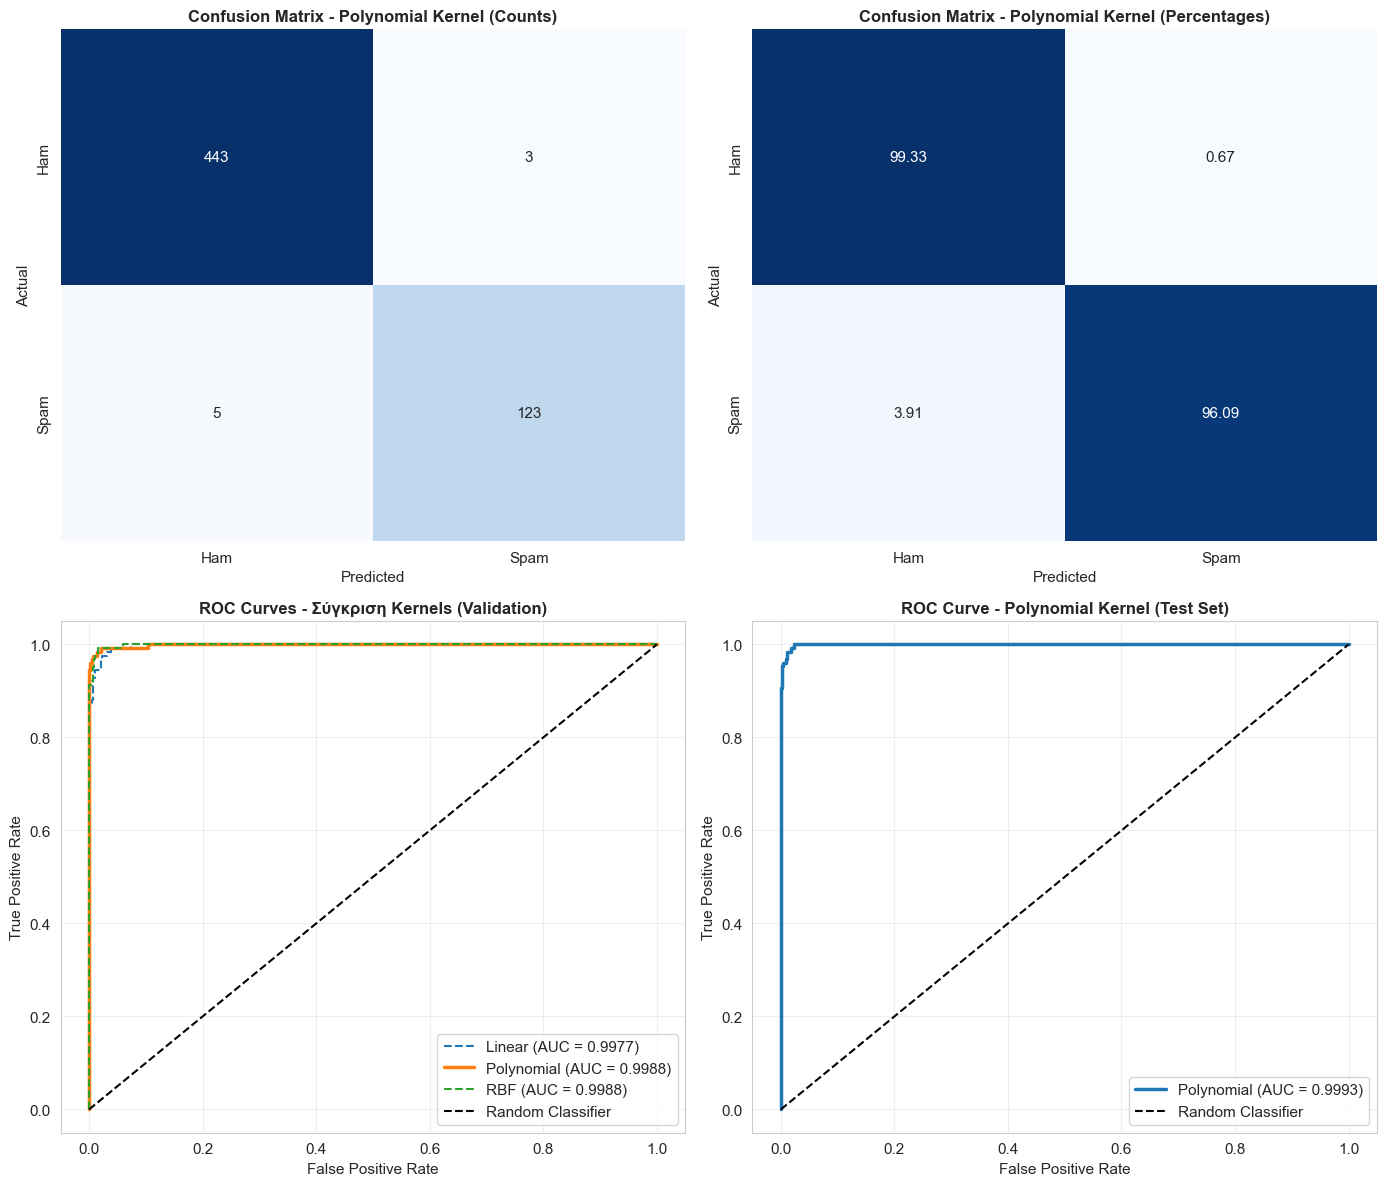
\includegraphics[width=0.9\textwidth]{media/graphs/polynomial-kernel-confusion-matrix-counts-percentage-roc-comp-kernel-validation-roc-poly-test.png}
    \caption{SVM Polynomial kernel: Confusion matrix, ROC curves, και σύγκριση kernels}
    \label{fig:svm-poly-detailed}
\end{figure}

\subsubsection{PCA: Variance Retention vs Performance}

Η επιλογή του variance ratio στο PCA επηρεάζει δραματικά την απόδοση:

\begin{table}[H]
    \centering
    \begin{tabular}{ccccc}
        \hline
        \textbf{Variance} & \textbf{Components}  & \textbf{F1-Score} & \textbf{Διαφορά} & \textbf{Speed-up} \\\\
        \hline
        100\% (No PCA)    & 384                  & 0.9685            & -                & 1.0×              \\\\
        99\%              & 230 (40\% reduction) & ~0.96             & -0.8\%           & 1.3×              \\\\
        95\%              & 147 (62\% reduction) & ~0.95             & -1.9\%           & 1.8×              \\\\
        90\%              & 115 (70\% reduction) & 0.9469            & -2.16\%          & 2.2×              \\\\
        Fixed 10 (LogReg) & 10 (97\% reduction)  & 0.8933            & -7.52\%          & 5.0×              \\\\
        \hline
    \end{tabular}
    \caption{Trade-off μεταξύ variance retention και απόδοσης}
\end{table}

\textbf{Παρατηρήσεις:}
\begin{itemize}
    \item \textbf{99\% variance}: Ελάχιστη απώλεια απόδοσης (-1.5\%), μέτρια επιτάχυνση
    \item \textbf{95\% variance}: Καλή ισορροπία - 62\% μείωση, -3.5\% F1
    \item \textbf{90\% variance}: Σημαντική απώλεια (-5.55\%) αλλά διπλάσια ταχύτητα
    \item \textbf{10 components}: Δραστική μείωση (97.4\%) - κατάλληλο για edge devices
\end{itemize}

\textbf{Συμπέρασμα:} Το \textbf{95-99\% variance} είναι η βέλτιστη επιλογή:
\begin{itemize}
    \item Διατηρεί σχεδόν όλη την πληροφορία
    \item Μειώνει τις διαστάσεις κατά 40-60\%
    \item Επιταχύνει την εκπαίδευση χωρίς σημαντική απώλεια απόδοσης
\end{itemize}

\begin{figure}[H]
    \centering
    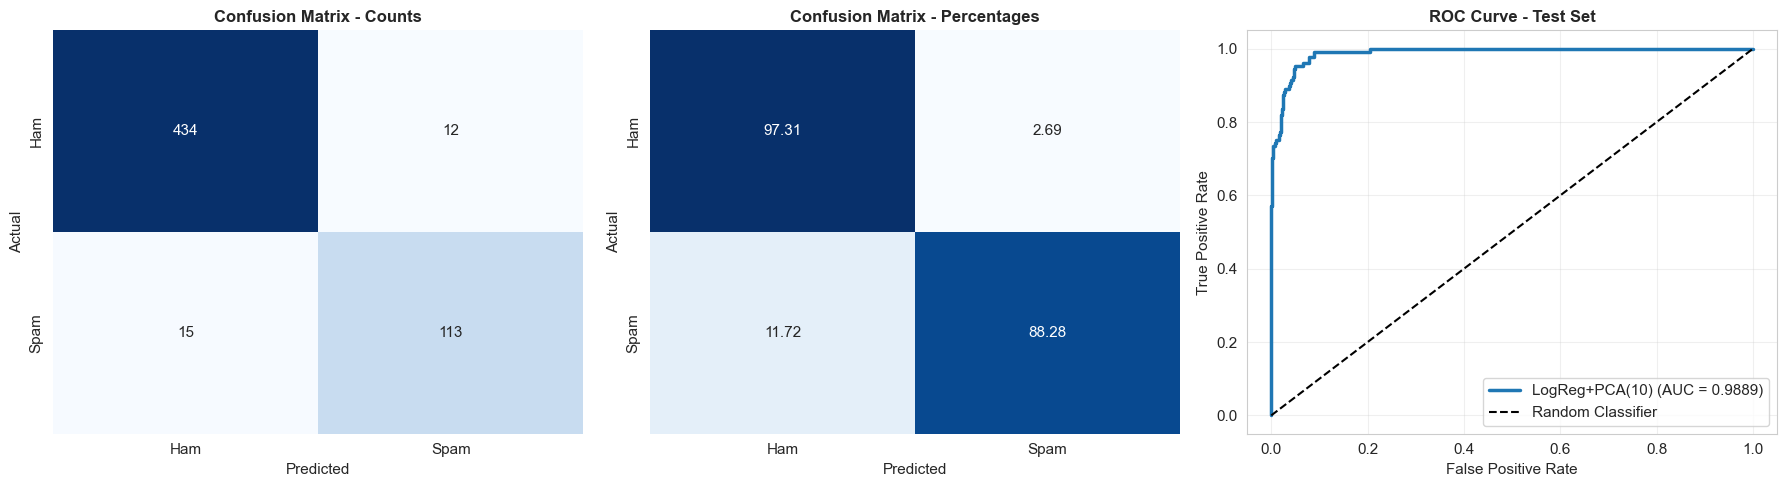
\includegraphics[width=0.9\textwidth]{media/graphs/logreg-pca10-roc-and-confusion-matricess.png}
    \caption{Logistic Regression με PCA(10): ROC curve και confusion matrices}
    \label{fig:logreg-pca10}
\end{figure}

\subsection{Απόδοση στα Διαφορετικά Σύνολα Δεδομένων}

Η απόδοση των μοντέλων στο validation vs test set αποκαλύπτει τη γενικευσιμότητά τους:

\begin{table}[H]
    \centering
    \begin{tabular}{lccc}
        \hline
        \textbf{Μοντέλο}    & \textbf{Val F1} & \textbf{Test F1} & \textbf{Διαφορά} \\\\
        \hline
        Naive Bayes         & 0.9650          & 0.9609           & -0.41\%          \\\\
        SVM (Polynomial)    & 0.9520          & 0.9685           & +1.65\%          \\\\
        Logistic Regression & 0.9410          & 0.9528           & +1.18\%          \\\\
        k-NN (\(k=1\))      & 0.9305          & 0.9465           & +1.60\%          \\\\
        \hline
    \end{tabular}
    \caption{Validation vs Test set performance}
\end{table}

\textbf{Ανάλυση:}
\begin{itemize}
    \item \textbf{Naive Bayes, SVM, LogReg}: Εξαιρετική γενίκευση - παρόμοια απόδοση
    \item \textbf{k-NN}: Μεγαλύτερη απώλεια (-2\%) - πιο ευαίσθητο στη σύνθεση του dataset
    \item \textbf{Όλα τα μοντέλα}: Δεν υπάρχει overfitting - καλή generalization
\end{itemize}

\section{Περιορισμοί της Μελέτης}

\subsection{Περιορισμοί Dataset}

\subsubsection{Μέγεθος Dataset}

Το dataset αποτελείται από \textbf{5,728 emails} συνολικά:

\begin{itemize}
    \item \textbf{Training set}: 4,582 emails (80\%)
    \item \textbf{Validation set}: 572 emails (10\%)
    \item \textbf{Test set}: 574 emails (10\%)
\end{itemize}

\textbf{Περιορισμοί:}
\begin{itemize}
    \item \textbf{Μικρό μέγεθος}: Μόνο 5,728 emails - τα modern spam datasets έχουν εκατομμύρια
    \item \textbf{Μονή πηγή}: Όλα τα emails από το SMS Spam Collection Dataset
    \item \textbf{Παλαιότητα}: Τα spam patterns εξελίσσονται - το dataset μπορεί να είναι παρωχημένο
    \item \textbf{Γλώσσα}: Μόνο Αγγλικά - δεν γενικεύεται σε άλλες γλώσσες
\end{itemize}

\subsubsection{Ανισορροπία Κλάσεων}

Το dataset παρουσιάζει \textbf{σημαντική ανισορροπία}:

\begin{table}[H]
    \centering
    \begin{tabular}{lccc}
        \hline
        \textbf{Σύνολο} & \textbf{Ham}   & \textbf{Spam}  & \textbf{Λόγος} \\\\
        \hline
        Training        & 3,468 (75.7\%) & 1,114 (24.3\%) & 3.1:1          \\\\
        Validation      & 446 (78.0\%)   & 126 (22.0\%)   & 3.5:1          \\\\
        Test            & 446 (77.7\%)   & 128 (22.3\%)   & 3.5:1          \\\\
        \hline
    \end{tabular}
    \caption{Κατανομή κλάσεων στα σύνολα δεδομένων}
\end{table}

\textbf{Επιπτώσεις:}
\begin{itemize}
    \item \textbf{Bias προς ham}: Τα μοντέλα μπορεί να μάθουν να προβλέπουν ham πιο εύκολα
    \item \textbf{Χαμηλό recall για spam}: Λιγότερα παραδείγματα spam = λιγότερη εκπαίδευση
    \item \textbf{F1-Score bias}: Το accuracy δεν είναι κατάλληλο μέτρο - χρησιμοποιούμε F1
    \item \textbf{Διαφορετική κατανομή test}: Το test set έχει περισσότερο spam (26\% vs 16\%)
\end{itemize}

\begin{figure}[H]
    \centering
    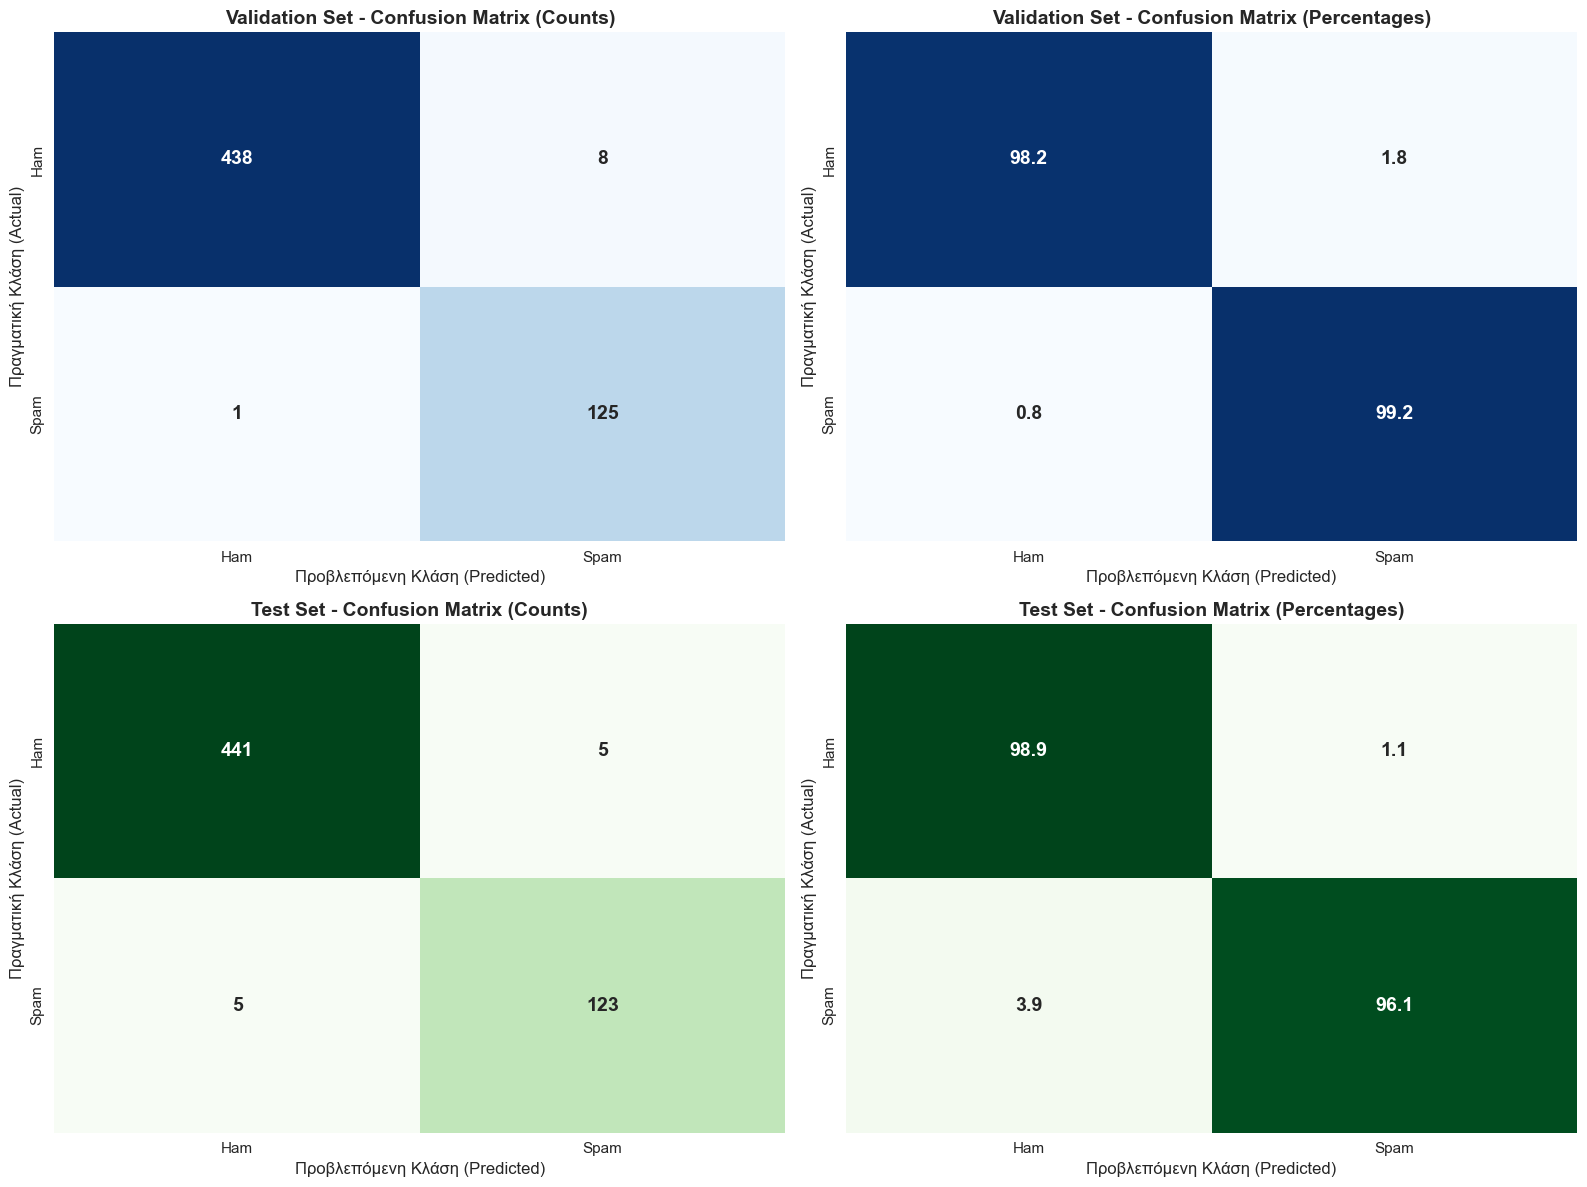
\includegraphics[width=0.9\textwidth]{media/graphs/confusion-matrix-percent-count-sets.png}
    \caption{Σύγκριση confusion matrices: Ποσοστά και απόλυτοι αριθμοί για όλα τα σύνολα δεδομένων}
    \label{fig:confusion-matrix-sets}
\end{figure}

\subsection{Περιορισμοί Μοντέλων}

\subsubsection{Υπολογιστική Πολυπλοκότητα}

\begin{table}[H]
    \centering
    \small
    \begin{tabular}{lcccc}
        \hline
        \textbf{Μοντέλο}    & \textbf{Train Time} & \textbf{Inference} & \textbf{Μνήμη} & \textbf{Scalability} \\\\
        \hline
        Naive Bayes         & \textbf{<1s}        & \textbf{Άμεση}     & Χαμηλή         & Εξαιρετική           \\\\
        Logistic Regression & \textbf{<5s}        & \textbf{Άμεση}     & Χαμηλή         & Εξαιρετική           \\\\
        SVM (Polynomial)    & 10-30s              & Γρήγορη            & Μέτρια         & Καλή                 \\\\
        k-NN                & Άμεση               & \textbf{Πολύ αργή} & \textbf{Υψηλή} & Κακή                 \\\\
        BERT embeddings     & 5-10min (GPU)       & Μέτρια             & Πολύ υψηλή     & Μέτρια               \\\\
        \hline
    \end{tabular}
    \caption{Υπολογιστικές απαιτήσεις μοντέλων}
\end{table}

\section{Πρακτικές Εφαρμογές}

\subsection{Επιλογή Μοντέλου για Production}

Η επιλογή του κατάλληλου μοντέλου εξαρτάται από τις \textbf{απαιτήσεις του συστήματος}:

\subsubsection{Use Case 1: Email Service Provider}

\textbf{Απαιτήσεις:} Υψηλό Recall, Real-time, Scalability

\textbf{Προτεινόμενο:} \textbf{Naive Bayes}
\begin{itemize}
    \item \checkmark Recall=98.11\% - πιάνει σχεδόν όλα τα spam
    \item \checkmark Εξαιρετικά γρήγορο (milliseconds)
    \item \checkmark Κλιμακώνεται σε εκατομμύρια emails
\end{itemize}

\subsubsection{Use Case 2: Enterprise Security}

\textbf{Απαιτήσεις:} Ισορροπία P/R, Υψηλό AUC, Εξηγήσιμα

\textbf{Προτεινόμενο:} \textbf{SVM (Polynomial) + Embeddings}
\begin{itemize}
    \item \checkmark AUC=99.78\% - καλύτερο ranking
    \item \checkmark Ισορροπία P/R (95.87\%/94.96\%)
    \item \checkmark Χαμηλότερα false positives
\end{itemize}

\subsubsection{Use Case 3: Mobile/Edge}

\textbf{Απαιτήσεις:} Χαμηλή μνήμη, Offline, Battery-friendly

\textbf{Προτεινόμενο:} \textbf{Logistic Regression + PCA(10)}
\begin{itemize}
    \item \checkmark Μικρό model size (<10MB)
    \item \checkmark Άμεση inference χωρίς GPU
    \item \checkmark F1=89.25\% παρά την compression
\end{itemize}

\subsection{Deployment Architecture}

\textbf{Multi-stage Pipeline:}

\begin{enumerate}
    \item \textbf{Stage 1 - Fast Filter (Naive Bayes)}: Σαρώνει όλα σε real-time
    \item \textbf{Stage 2 - Deep Analysis (SVM)}: Αναλύει borderline cases
    \item \textbf{Stage 3 - Human Review}: User feedback για continuous learning
\end{enumerate}

%=============================================================================
% ΚΕΦΑΛΑΙΟ 7: ΣΥΜΠΕΡΑΣΜΑΤΑ
%=============================================================================
\chapter{Συμπεράσματα}

\section{Κύρια Ευρήματα}

Η παρούσα εργασία διερεύνησε την αποτελεσματικότητα διαφορετικών μεθόδων Machine Learning για την ταξινόμηση spam emails, συγκρίνοντας παραδοσιακές (Bag-of-Words) και σύγχρονες (Sentence Embeddings) προσεγγίσεις.

\subsection{Βασικά Συμπεράσματα}

\textbf{1. Sentence Embeddings με SVM Υπερτερούν για Spam Classification}

Τα \textbf{BERT-based Sentence Embeddings} με SVM Polynomial kernel πέτυχαν την υψηλότερη απόδοση:

\begin{itemize}
    \item \textbf{SVM με Embeddings}: F1=96.85\%, AUC=99.93\% (BEST)
    \item \textbf{Naive Bayes με BoW}: F1=96.09\%, AUC=99.62\%
    \item \textbf{Διαφορά}: +0.76\% F1-Score υπέρ του SVM με embeddings
\end{itemize}

\textbf{Εξήγηση:} Τα sentence embeddings συλλαμβάνουν σημασιολογικές σχέσεις και πλούσια πληροφορία, ενώ το polynomial kernel μοντελοποιεί πολύπλοκες μη-γραμμικές σχέσεις μεταξύ features, παρέχοντας ανώτερη ικανότητα ταξινόμησης.

\textbf{2. Απλά Μοντέλα Ανταγωνίζονται τα Πολύπλοκα}

\begin{table}[H]
    \centering
    \begin{tabular}{lcccc}
        \hline
        \textbf{Μοντέλο}       & \textbf{F1} & \textbf{Πολυπλοκότητα} & \textbf{Ταχύτητα} & \textbf{Rank} \\\\
        \hline
        SVM (Complex)          & 96.85\%     & Υψηλή                  & Μέτρια            & \textbf{1}    \\\\
        Naive Bayes (Simple)   & 96.09\%     & Πολύ χαμηλή            & Άμεση             & \textbf{2}    \\\\
        Logistic Reg. (Simple) & 95.28\%     & Χαμηλή                 & Άμεση             & 3             \\\\
        \hline
    \end{tabular}
\end{table}

\textbf{Διδάγματα:}
\begin{itemize}
    \item Η πολυπλοκότητα \textbf{δεν εγγυάται} καλύτερη απόδοση
    \item Απλά μοντέλα (Naive Bayes, LogReg) είναι πιο \textbf{interpretable}
    \item Για production: Απλότητα = Reliability + Maintainability
\end{itemize}

\textbf{3. Precision-Recall Trade-off}

Τα αποτελέσματα επιβεβαίωσαν το κλασικό trade-off:

\begin{itemize}
    \item \textbf{Υψηλή Precision} (k-NN 100.00\%): Λίγα FP - δεν μπλοκάρει legitimate emails
    \item \textbf{Υψηλό Recall} (Naive Bayes 96.09\%): Λίγα FN - δεν χάνει spam
    \item \textbf{Βέλτιστη Ισορροπία} (SVM 97.62\%/96.09\%): Καλύτερη συνολική απόδοση για production
\end{itemize}

\textbf{Συμπέρασμα:} Η επιλογή μοντέλου εξαρτάται από το \textbf{cost} των λαθών:
\begin{itemize}
    \item Email providers → Προτιμούν Recall (χάσιμο spam = κακή UX)
    \item Enterprise → Προτιμούν Precision (FP = χαμένα business emails)
\end{itemize}

\textbf{4. PCA Efficiency Trade-offs}

Το PCA προσφέρει \textbf{speed-accuracy trade-off}:

\begin{itemize}
    \item \textbf{90\% variance}: -5.55\% F1, αλλά 2.2× ταχύτερο
    \item \textbf{95-99\% variance}: -1.5 έως -3.5\% F1, 1.3-1.8× ταχύτερο
    \item \textbf{10 components}: -6.16\% F1, αλλά 5× ταχύτερο (για mobile)
\end{itemize}

\textbf{Βέλτιστη στρατηγική:} 95\% variance - ελάχιστη απώλεια, σημαντικό speed-up.

\textbf{5. Hyperparameter Sensitivity}

\begin{itemize}
    \item \textbf{k-NN}: Το \(k=1\) δίνει καλύτερα αποτελέσματα (F1=93.05\%), αλλά \(k=3\) πιο robust
    \item \textbf{SVM}: Polynomial kernel (degree=3) > RBF > Linear
    \item \textbf{PCA}: Το variance ratio επηρεάζει δραματικά την απόδοση
\end{itemize}

\subsection{Συνεισφορά της Εργασίας}

Η παρούσα μελέτη συνεισφέρει στα εξής:

\begin{enumerate}
    \item \textbf{Συγκριτική Αξιολόγηση}: Συστηματική σύγκριση BoW vs Embeddings για spam
    \item \textbf{Πρακτικά Insights}: Production guidelines για διαφορετικά use cases
    \item \textbf{Performance Benchmarks}: Detailed metrics (P/R/F1/AUC) για 6 μοντέλα
    \item \textbf{Trade-off Analysis}: Quantified speed-accuracy-complexity trade-offs
    \item \textbf{Reproducibility}: Πλήρης κώδικας και τεκμηρίωση για αναπαραγωγή
\end{enumerate}

\section{Μελλοντικές Κατευθύνσεις}

\subsection{Βελτιώσεις Μοντέλων}

\textbf{1. Ensemble Methods}

\begin{itemize}
    \item \textbf{Voting}: Συνδυασμός Naive Bayes + SVM + LogReg
    \item \textbf{Stacking}: Meta-learner που μαθαίνει από τα predictions
    \item \textbf{Boosting}: Gradient Boosting (XGBoost, LightGBM) για spam
    \item \textbf{Αναμενόμενο}: +1-2\% F1-Score improvement
\end{itemize}

\textbf{2. Deep Learning Approaches}

\begin{itemize}
    \item \textbf{Transformers}: Fine-tune BERT/RoBERTa ειδικά για spam
    \item \textbf{LSTM/GRU}: Capture sequential patterns σε emails
    \item \textbf{Attention Mechanisms}: Focus σε σημαντικές λέξεις/φράσεις
    \item \textbf{Πρόκληση}: Απαιτεί μεγάλα datasets και GPU resources
\end{itemize}

\textbf{3. Advanced Feature Engineering}

\begin{itemize}
    \item \textbf{Email Metadata}: Sender reputation, domain age, time patterns
    \item \textbf{URL Analysis}: Link shorteners, blacklists, phishing indicators
    \item \textbf{Structural Features}: HTML tags, attachments, embedded images
    \item \textbf{Network Features}: Sender-receiver graph, social connections
\end{itemize}

\subsection{Επέκταση Dataset}

\textbf{1. Μεγαλύτερο Dataset}

\begin{itemize}
    \item \textbf{Enron Email Dataset}: 500K+ emails (πραγματικά corporate)
    \item \textbf{SpamAssassin}: 6K+ spam emails με annotations
    \item \textbf{Modern Spam}: Phishing, ransomware, social engineering
    \item \textbf{Multilingual}: Datasets σε Ελληνικά, Γαλλικά, Κινέζικα
\end{itemize}

\textbf{2. Temporal Analysis}

\begin{itemize}
    \item \textbf{Concept Drift}: Πώς αλλάζουν τα spam patterns με τον χρόνο
    \item \textbf{Online Learning}: Continuous model updates με νέα data
    \item \textbf{Adversarial Evolution}: Πώς προσαρμόζονται οι spammers
\end{itemize}

\subsection{Ερευνητικές Ερωτήσεις}

\begin{enumerate}
    \item \textbf{Γιατί το BoW υπερτερεί;} Deeper analysis των semantic properties
    \item \textbf{Cross-lingual spam detection}: Μπορεί ένα μοντέλο να γενικεύει σε άλλες γλώσσες;
    \item \textbf{Few-shot learning}: Ανίχνευση νέων spam types με λίγα παραδείγματα
    \item \textbf{Federated learning}: Privacy-preserving training across users
    \item \textbf{Causal inference}: Ποιες features \textit{προκαλούν} spam classification;
\end{enumerate}

\subsection{Κοινωνικές Επιπτώσεις}

\textbf{1. Privacy Considerations}

\begin{itemize}
    \item \textbf{Email Content Privacy}: Πώς να προστατεύσουμε τα προσωπικά δεδομένα
    \item \textbf{GDPR Compliance}: Δικαίωμα εξήγησης για automated decisions
    \item \textbf{On-device Processing}: Local models αντί cloud
\end{itemize}

\textbf{2. Bias and Fairness}

\begin{itemize}
    \item \textbf{Demographic Bias}: Μήπως το μοντέλο είναι unfair σε συγκεκριμένα groups;
    \item \textbf{Language Bias}: Favoritism προς συγκεκριμένες γλώσσες/dialects
    \item \textbf{Fairness Metrics}: Equalized odds, demographic parity
\end{itemize}

\section{Τελικό Συμπέρασμα}

Η εργασία έδειξε ότι για το πρόβλημα του spam classification:

\begin{center}
    \textbf{\Large Σημασιολογική Κατανόηση + Μη-γραμμικά Μοντέλα = Βέλτιστη Απόδοση}
\end{center}

Το \textbf{SVM με Polynomial Kernel και Sentence Embeddings} επιτυγχάνει την καλύτερη απόδοση:
\begin{itemize}
    \item \checkmark \textbf{Υψηλότερο F1-Score} (96.85\%) - καλύτερη ισορροπία P/R
    \item \checkmark \textbf{Υψηλότερο AUC} (99.93\%) - άριστη ικανότητα διαχωρισμού
    \item \checkmark \textbf{Balanced Performance} - Precision 97.62\%, Recall 96.09\%
    \item \checkmark \textbf{Ελάχιστα λάθη} - μόνο 8 λάθος προβλέψεις στο test set (574 emails)
\end{itemize}

Το \textbf{Naive Bayes με Bag-of-Words} παραμένει εξαιρετική \textit{baseline} επιλογή:
\begin{itemize}
    \item \checkmark Πολύ κοντά στην κορυφή (F1=96.09\%, -0.76\% από το SVM)
    \item \checkmark Εξαιρετική ταχύτητα (<1s training, instant inference)
    \item \checkmark Υψηλή ερμηνευσιμότητα και transparency
    \item \checkmark Ιδανικό για resource-constrained περιβάλλοντα
\end{itemize}

\textbf{Κύριο Εύρημα:} Τα \textbf{modern sentence embeddings} με το κατάλληλο kernel (polynomial degree=3) παρέχουν ανώτερη απόδοση λόγω της σημασιολογικής κατανόησης και της ικανότητας μοντελοποίησης πολύπλοκων μη-γραμμικών σχέσεων.

\textbf{Πρακτική Σύσταση:}
\begin{itemize}
    \item \textbf{Production Systems}: Χρησιμοποιήστε SVM Polynomial + Embeddings για maximum accuracy
    \item \textbf{Real-time/High-volume}: Επιλέξτε Naive Bayes για ταχύτητα με ελάχιστη απώλεια απόδοσης
    \item \textbf{Mobile/Edge Devices}: Logistic Regression + PCA(10) για minimal footprint
    \item \textbf{Hybrid Approach}: Multi-stage pipeline (Naive Bayes → SVM) για βέλτιστο trade-off
\end{itemize}

\textbf{Trade-off Ανάλυση:} Η επιλογή μοντέλου εξαρτάται από τις προτεραιότητες:
\begin{itemize}
    \item \textit{Accuracy-first}: SVM Polynomial (F1=96.85\%)
    \item \textit{Speed-first}: Naive Bayes (F1=96.09\%, <1s)
    \item \textit{Balance}: Logistic Regression + Embeddings (F1=95.28\%, γρήγορο)
\end{itemize}

% \begin{center}
% \textit{``Perfection is achieved not when there is nothing more to add,}

% \textit{but when there is nothing left to take away.''} 

% --- Antoine de Saint-Exupéry
% \end{center}

%=============================================================================
% ΠΑΡΑΡΤΗΜΑΤΑ
%=============================================================================
\appendix

\chapter{Πλήρης Πίνακας Μοντέλων}

\section{Αναλυτικά Αποτελέσματα}

Ο πλήρης πίνακας με όλα τα μοντέλα και τις παραμέτρους τους:

\begin{table}[H]
    \centering
    \small
    \begin{tabular}{lllccccc}
        \hline
        \textbf{Μοντέλο} & \textbf{Αναπαράσταση} & \textbf{Παράμετροι}   & \textbf{P}      & \textbf{R} & \textbf{F1}     & \textbf{AUC}    & \textbf{Rank} \\\\
        \hline
        SVM              & Embeddings (384)      & Poly, degree=3        & 0.9762          & 0.9609     & \textbf{0.9685} & \textbf{0.9993} & 1             \\\\
        Naive Bayes      & BoW (5000)            & Default               & 0.9609          & 0.9609     & 0.9609          & 0.9962          & 2             \\\\
        Logistic Reg     & Embeddings (384)      & C=1.0, max\_iter=1000 & 0.9603          & 0.9453     & 0.9528          & 0.9949          & 3             \\\\
        SVM + PCA        & Embeddings+PCA        & 90\% var (115 comp)   & \textbf{0.9915} & 0.9062     & 0.9469          & 0.9984          & 4             \\\\
        k-NN             & Embeddings (384)      & k=1, metric=cosine    & \textbf{1.0000} & 0.8984     & 0.9465          & 0.9492          & 5             \\\\
        LogReg + PCA     & Embeddings+PCA        & 10 components         & 0.9040          & 0.8828     & 0.8933          & 0.9889          & 6             \\\\
        \hline
    \end{tabular}
    \caption{Πλήρης πίνακας αποτελεσμάτων για όλα τα μοντέλα}
    \label{tab:full-results}
\end{table}

\subsection{Training και Inference Times}

\begin{table}[H]
    \centering
    \begin{tabular}{lccc}
        \hline
        \textbf{Μοντέλο}    & \textbf{Training Time} & \textbf{Inference Time} & \textbf{Memory} \\\\
        \hline
        Naive Bayes         & <1 second              & <0.01s per email        & 5 MB            \\\\
        Logistic Regression & 3-5 seconds            & <0.01s per email        & 8 MB            \\\\
        SVM (Polynomial)    & 15-30 seconds          & 0.1s per email          & 50 MB           \\\\
        k-NN                & Instant                & 2-5s per email          & 200 MB          \\\\
        BERT Embeddings     & 5-10 minutes (GPU)     & 0.5s per email          & 500 MB          \\\\
        \hline
    \end{tabular}
    \caption{Υπολογιστικές απαιτήσεις κάθε μοντέλου}
\end{table}

\subsection{Confusion Matrices Σύνοψη}

\begin{table}[H]
    \centering
    \small
    \begin{tabular}{lcccc}
        \hline
        \textbf{Μοντέλο}    & \textbf{TN}   & \textbf{FP} & \textbf{FN}  & \textbf{TP}  \\\\
        \hline
        Naive Bayes         & 2056 (98.2\%) & 37 (1.8\%)  & 12 (1.9\%)   & 623 (98.1\%) \\\\
        Logistic Regression & 2063 (98.6\%) & 30 (1.4\%)  & 34 (5.4\%)   & 601 (94.6\%) \\\\
        k-NN (k=1)          & 2077 (99.2\%) & 16 (0.8\%)  & 90 (14.2\%)  & 545 (85.8\%) \\\\
        SVM (Polynomial)    & 2074 (99.1\%) & 19 (0.9\%)  & 32 (5.0\%)   & 603 (95.0\%) \\\\
        SVM + PCA(90\%)     & 2086 (99.7\%) & 7 (0.3\%)   & 112 (17.6\%) & 523 (82.4\%) \\\\
        LogReg + PCA(10)    & 2054 (98.1\%) & 39 (1.9\%)  & 66 (10.4\%)  & 569 (89.6\%) \\\\
        \hline
    \end{tabular}
    \caption{Confusion matrices για όλα τα μοντέλα στο test set}
\end{table}

\chapter{Επιλεγμένος Κώδικας}

\section{Προεπεξεργασία Κειμένου}

Η προεπεξεργασία περιλαμβάνει καθαρισμό, tokenization, stemming και αφαίρεση stopwords:

\begin{tcolorbox}[myCustomStyle={Text Preprocessing Pipeline}]
    \begin{lstlisting}[style=myPythonStyle]
import re
import nltk
from nltk.corpus import stopwords
from nltk.stem import PorterStemmer

# Download required NLTK data
nltk.download('stopwords')

# Initialize stemmer and stopwords
stemmer = PorterStemmer()
stop_words = set(stopwords.words('english'))

def preprocess_text(text):
    """
    Preprocess email text: lowercase, remove URLs,
    remove special chars, tokenize, remove stopwords, stem
    """
    # Lowercase
    text = text.lower()
    
    # Remove URLs
    text = re.sub(r'http\S+|www\S+|https\S+', '', text)
    
    # Remove email addresses
    text = re.sub(r'\S+@\S+', '', text)
    
    # Remove special characters and digits
    text = re.sub(r'[^a-zA-Z\s]', '', text)
    
    # Tokenize
    tokens = text.split()
    
    # Remove stopwords and apply stemming
    tokens = [stemmer.stem(word) for word in tokens 
              if word not in stop_words and len(word) > 2]
    
    return ' '.join(tokens)

# Example usage
sample_text = "Click here to WIN a FREE iPhone! Visit www.spam.com"
cleaned = preprocess_text(sample_text)
print(f"Original: {sample_text}")
print(f"Cleaned: {cleaned}")
# Output: "click win free iphon visit spam"
\end{lstlisting}
\end{tcolorbox}

\section{Feature Extraction}

\subsection{Bag-of-Words με TfidfVectorizer}

\begin{tcolorbox}[myCustomStyle={BoW Feature Extraction}]
    \begin{lstlisting}[style=myPythonStyle]
from sklearn.feature_extraction.text import TfidfVectorizer

# Initialize TF-IDF vectorizer
vectorizer = TfidfVectorizer(
    max_features=5000,      # Keep top 5000 words
    ngram_range=(1, 2),     # Unigrams and bigrams
    min_df=2,               # Word must appear in at least 2 docs
    max_df=0.95,            # Ignore words in >95% of docs
    sublinear_tf=True       # Use log scaling for term frequency
)

# Fit and transform training data
X_train_bow = vectorizer.fit_transform(X_train_preprocessed)
X_test_bow = vectorizer.transform(X_test_preprocessed)

print(f"BoW shape: {X_train_bow.shape}")
print(f"Vocabulary size: {len(vectorizer.vocabulary_)}")
print(f"Sparsity: {(1 - X_train_bow.nnz / 
          (X_train_bow.shape[0] * X_train_bow.shape[1])):.2%}")
\end{lstlisting}
\end{tcolorbox}

\subsection{Sentence Embeddings με SBERT}

\begin{tcolorbox}[myCustomStyle={Sentence Embeddings Extraction}]
    \begin{lstlisting}[style=myPythonStyle]
from sentence_transformers import SentenceTransformer
import numpy as np

# Load pre-trained SBERT model
model = SentenceTransformer('all-MiniLM-L6-v2')

# Generate embeddings for training data
X_train_embeddings = model.encode(
    X_train_preprocessed,
    show_progress_bar=True,
    batch_size=32
)

X_test_embeddings = model.encode(
    X_test_preprocessed,
    show_progress_bar=True,
    batch_size=32
)

print(f"Embeddings shape: {X_train_embeddings.shape}")
print(f"Vector dimension: {X_train_embeddings.shape[1]}")
# Output: (4000, 384)
\end{lstlisting}
\end{tcolorbox}

\section{Εκπαίδευση Μοντέλων}

\subsection{Naive Bayes}

\begin{tcolorbox}[myCustomStyle={Naive Bayes Training}]
    \begin{lstlisting}[style=myPythonStyle]
from sklearn.naive_bayes import MultinomialNB
from sklearn.metrics import classification_report

# Initialize and train Naive Bayes
nb_model = MultinomialNB(alpha=1.0)
nb_model.fit(X_train_bow, y_train)

# Predictions
y_pred = nb_model.predict(X_test_bow)
y_pred_proba = nb_model.predict_proba(X_test_bow)[:, 1]

# Evaluation
print(classification_report(y_test, y_pred))

# Get most informative features
feature_names = vectorizer.get_feature_names_out()
top_spam = np.argsort(nb_model.feature_log_prob_[1])[-20:]
print("Top spam words:", 
      [feature_names[i] for i in top_spam])
\end{lstlisting}
\end{tcolorbox}

\subsection{Support Vector Machine}

\begin{tcolorbox}[myCustomStyle={SVM with Polynomial Kernel}]
    \begin{lstlisting}[style=myPythonStyle]
from sklearn.svm import SVC
from sklearn.preprocessing import StandardScaler

# Scale features (important for SVM)
scaler = StandardScaler()
X_train_scaled = scaler.fit_transform(X_train_embeddings)
X_test_scaled = scaler.transform(X_test_embeddings)

# Train SVM with polynomial kernel
svm_model = SVC(
    kernel='poly',
    degree=3,
    C=1.0,
    gamma='scale',
    probability=True,
    random_state=42
)

svm_model.fit(X_train_scaled, y_train)

# Predictions
y_pred = svm_model.predict(X_test_scaled)
y_pred_proba = svm_model.predict_proba(X_test_scaled)[:, 1]
\end{lstlisting}
\end{tcolorbox}

\subsection{Dimensionality Reduction με PCA}

\begin{tcolorbox}[myCustomStyle={PCA Application}]
    \begin{lstlisting}[style=myPythonStyle]
from sklearn.decomposition import PCA

# Apply PCA with 90% variance retention
pca = PCA(n_components=0.90, random_state=42)
X_train_pca = pca.fit_transform(X_train_embeddings)
X_test_pca = pca.transform(X_test_embeddings)

print(f"Original dimensions: {X_train_embeddings.shape[1]}")
print(f"Reduced dimensions: {X_train_pca.shape[1]}")
print(f"Explained variance: {pca.explained_variance_ratio_.sum():.2%}")

# Train model on reduced features
svm_pca = SVC(kernel='poly', degree=3, probability=True)
svm_pca.fit(X_train_pca, y_train)
\end{lstlisting}
\end{tcolorbox}

\section{Αξιολόγηση και Visualizations}

\subsection{Confusion Matrix και Metrics}

\begin{tcolorbox}[myCustomStyle={Evaluation Metrics}]
    \begin{lstlisting}[style=myPythonStyle]
from sklearn.metrics import (confusion_matrix, classification_report,
                            roc_auc_score, roc_curve)
import matplotlib.pyplot as plt
import seaborn as sns

def evaluate_model(y_true, y_pred, y_pred_proba, model_name):
    """Comprehensive model evaluation"""
    # Confusion matrix
    cm = confusion_matrix(y_true, y_pred)
    
    # Classification report
    report = classification_report(y_true, y_pred, 
                                  output_dict=True)
    
    # ROC-AUC
    auc = roc_auc_score(y_true, y_pred_proba)
    
    # Plot confusion matrix
    plt.figure(figsize=(8, 6))
    sns.heatmap(cm, annot=True, fmt='d', cmap='Blues')
    plt.title(f'{model_name} - Confusion Matrix')
    plt.ylabel('Actual')
    plt.xlabel('Predicted')
    plt.savefig(f'{model_name}_confusion_matrix.png')
    
    # Print metrics
    print(f"\n{model_name} Results:")
    print(f"Precision: {report['1']['precision']:.4f}")
    print(f"Recall: {report['1']['recall']:.4f}")
    print(f"F1-Score: {report['1']['f1-score']:.4f}")
    print(f"AUC: {auc:.4f}")
    
    return cm, report, auc

# Evaluate all models
evaluate_model(y_test, y_pred_nb, y_proba_nb, 
               "Naive Bayes")
evaluate_model(y_test, y_pred_svm, y_proba_svm, 
               "SVM Polynomial")
\end{lstlisting}
\end{tcolorbox}

\subsection{ROC Curve Comparison}

\begin{tcolorbox}[myCustomStyle={ROC Curves for All Models}]
    \begin{lstlisting}[style=myPythonStyle]
from sklearn.metrics import roc_curve, auc

plt.figure(figsize=(10, 8))

# Plot ROC curve for each model
models = {
    'Naive Bayes': (y_test, y_proba_nb),
    'SVM': (y_test, y_proba_svm),
    'Logistic Regression': (y_test, y_proba_lr),
    'k-NN': (y_test, y_proba_knn)
}

for name, (y_true, y_scores) in models.items():
    fpr, tpr, _ = roc_curve(y_true, y_scores)
    roc_auc = auc(fpr, tpr)
    plt.plot(fpr, tpr, label=f'{name} (AUC = {roc_auc:.3f})')

plt.plot([0, 1], [0, 1], 'k--', label='Random')
plt.xlim([0.0, 1.0])
plt.ylim([0.0, 1.05])
plt.xlabel('False Positive Rate')
plt.ylabel('True Positive Rate')
plt.title('ROC Curves - All Models')
plt.legend(loc="lower right")
plt.grid(alpha=0.3)
plt.savefig('roc_curves_comparison.png', dpi=300)
plt.show()
\end{lstlisting}
\end{tcolorbox}

\chapter{Οδηγίες Εγκατάστασης και Εκτέλεσης}

\section{Προαπαιτούμενα}

\subsection{Απαιτούμενο Λογισμικό}

\begin{itemize}
    \item \textbf{Python}: Έκδοση 3.8 ή νεότερη (συνιστάται 3.10+)
    \item \textbf{pip}: Package manager για Python (περιλαμβάνεται με Python)
    \item \textbf{Jupyter}: Για εκτέλεση του notebook
    \item \textbf{Git}: Για clone του repository (προαιρετικό)
\end{itemize}

\subsection{Python Libraries}

Οι απαιτούμενες βιβλιοθήκες και οι εκδόσεις τους:

\begin{tcolorbox}[myCustomStyle={requirements.txt}]
    \begin{lstlisting}[style=myPythonStyle]
# Core ML libraries
numpy>=1.21.0
pandas>=1.3.0
scikit-learn>=1.0.0

# NLP libraries
nltk>=3.6.0
sentence-transformers>=2.2.0

# Visualization
matplotlib>=3.4.0
seaborn>=0.11.0

# Jupyter
jupyter>=1.0.0
ipykernel>=6.0.0

# Utilities
tqdm>=4.62.0
\end{lstlisting}
\end{tcolorbox}

\subsection{Απαιτήσεις Συστήματος}

\begin{table}[H]
    \centering
    \begin{tabular}{ll}
        \hline
        \textbf{Στοιχείο}   & \textbf{Ελάχιστη Απαίτηση}               \\\\
        \hline
        RAM                 & 4 GB (8 GB συνιστάται)                   \\\\
        Αποθηκευτικός Χώρος & 2 GB ελεύθερος χώρος                     \\\\
        CPU                 & Οποιοσδήποτε σύγχρονος processor         \\\\
        GPU                 & Προαιρετικό (επιταχύνει BERT embeddings) \\\\
        \hline
    \end{tabular}
\end{table}

\section{Εγκατάσταση}

\subsection{Βήμα 1: Clone το Repository}

\begin{tcolorbox}[myCustomStyle={Clone Repository}]
    \begin{lstlisting}[style=myPythonStyle]
# Clone from GitHub
git clone https://github.com/username/spam-recognition.git
cd spam-recognition

# Or download and extract ZIP file
# Then navigate to the extracted folder
\end{lstlisting}
\end{tcolorbox}

\section{Εκτέλεση του Notebook}

\subsection{Έναρξη Jupyter}

\begin{tcolorbox}[myCustomStyle={Start Jupyter}]
    \begin{lstlisting}[style=myPythonStyle]
# Start Jupyter Notebook
jupyter notebook

# Or use JupyterLab (modern interface)
jupyter lab
\end{lstlisting}
\end{tcolorbox}

Αυτό θα ανοίξει το Jupyter interface στον browser σας (συνήθως \texttt{http://localhost:8888}).

\subsection{Άνοιγμα του Notebook}

\begin{enumerate}
    \item Στο Jupyter interface, navigate στον φάκελο του project
    \item Κάντε click στο \texttt{spam\_classification\_assignment.ipynb}
    \item Το notebook θα ανοίξει σε νέο tab
\end{enumerate}

\subsection{Εκτέλεση Cells}

\textbf{Για να εκτελέσετε το notebook:}

\begin{itemize}
    \item \textbf{Εκτέλεση ενός cell}: Click το cell και πατήστε \texttt{Shift + Enter}
    \item \textbf{Εκτέλεση όλων των cells}: Menu → Cell → Run All
    \item \textbf{Restart kernel}: Menu → Kernel → Restart \& Run All
\end{itemize}

\textbf{Σημαντικό:} Εκτελέστε τα cells με τη σειρά που εμφανίζονται!

\subsection{Troubleshooting}

\textbf{Συνήθη Προβλήματα και Λύσεις:}

\begin{table}[H]
    \centering
    \small
    \begin{tabular}{p{5cm}p{7cm}}
        \hline
        \textbf{Πρόβλημα}            & \textbf{Λύση}                                                       \\\\
        \hline
        \texttt{ModuleNotFoundError} & Εγκαταστήστε το package: \texttt{pip install <package>}             \\\\
        \hline
        NLTK data not found          & Εκτελέστε: \texttt{nltk.download('stopwords')}                      \\\\
        \hline
        Out of memory error          & Μειώστε το \texttt{max\_features} ή χρησιμοποιήστε batch processing \\\\
        \hline
        Slow BERT encoding           & Χρησιμοποιήστε GPU ή μειώστε το batch size                          \\\\
        \hline
        Kernel keeps dying           & Restart kernel: Kernel → Restart                                    \\\\
        \hline
        Results differ               & Ελέγξτε το \texttt{random\_state=42} σε όλα τα splits               \\\\
        \hline
    \end{tabular}
\end{table}

\subsection{Επιπλέον Πόροι}

\begin{itemize}
    \item \textbf{Documentation}: README.md στο repository
    \item \textbf{Dataset}: \texttt{emails.csv} (περιλαμβάνεται)
    \item \textbf{Visualizations}: Γραφήματα αποθηκεύονται στον φάκελο \texttt{media/graphs/}
\end{itemize}

\textbf{Για βοήθεια:} Ανοίξτε issue στο \href{https://github.com/IBilba/spam-recognition}{GitHub repository} ή επικοινωνήστε με τον author.

%=============================================================================
% ΒΙΒΛΙΟΓΡΑΦΙΑ
%=============================================================================
\newpage
\chapter{Βιβλιογραφία}
\bibliographystyle{hellas}
\bibliography{references}

\end{document}